% Template for PLoS
% Version 3.6 Aug 2022
%
% % % % % % % % % % % % % % % % % % % % % %
%
% -- IMPORTANT NOTE
%
% This template contains comments intended
% to minimize problems and delays during our production
% process. Please follow the template instructions
% whenever possible.
%
% % % % % % % % % % % % % % % % % % % % % % %
%
% Once your paper is accepted for publication,
% PLEASE REMOVE ALL TRACKED CHANGES in this file
% and leave only the final text of your manuscript.
% PLOS recommends the use of latexdiff to track changes during review, as this will help to maintain a clean tex file.
% Visit https://www.ctan.org/pkg/latexdiff?lang=en for info or contact us at latex@plos.org.
%
%
% There are no restrictions on package use within the LaTeX files except that no packages listed in the template may be deleted.
%
% Please do not include colors or graphics in the text.
%
% The manuscript LaTeX source should be contained within a single file (do not use \input, \externaldocument, or similar commands).
%
% % % % % % % % % % % % % % % % % % % % % % %
%
% -- FIGURES AND TABLES
%
% Please include tables/figure captions directly after the paragraph where they are first cited in the text.
%
% DO NOT INCLUDE GRAPHICS IN YOUR MANUSCRIPT
% - Figures should be uploaded separately from your manuscript file.
% - Figures generated using LaTeX should be extracted and removed from the PDF before submission.
% - Figures containing multiple panels/subfigures must be combined into one image file before submission.
% For figure citations, please use "Fig" instead of "Figure".
% See http://journals.plos.org/plosone/s/figures for PLOS figure guidelines.
%
% Tables should be cell-based and may not contain:
% - spacing/line breaks within cells to alter layout or alignment
% - do not nest tabular environments (no tabular environments within tabular environments)
% - no graphics or colored text (cell background color/shading OK)
% See http://journals.plos.org/plosone/s/tables for table guidelines.
%
% For tables that exceed the width of the text column, use the adjustwidth environment as illustrated in the example table in text below.
%
% % % % % % % % % % % % % % % % % % % % % % % %
%
% -- EQUATIONS, MATH SYMBOLS, SUBSCRIPTS, AND SUPERSCRIPTS
%
% IMPORTANT
% Below are a few tips to help format your equations and other special characters according to our specifications. For more tips to help reduce the possibility of formatting errors during conversion, please see our LaTeX guidelines at http://journals.plos.org/plosone/s/latex
%
% For inline equations, please be sure to include all portions of an equation in the math environment.  For example, x$^2$ is incorrect; this should be formatted as $x^2$ (or $\mathrm{x}^2$ if the romanized font is desired).
%
% Do not include text that is not math in the math environment. For example, CO2 should be written as CO\textsubscript{2} instead of CO$_2$.
%
% Please add line breaks to long display equations when possible in order to fit size of the column.
%
% For inline equations, please do not include punctuation (commas, etc) within the math environment unless this is part of the equation.
%
% When adding superscript or subscripts outside of brackets/braces, please group using {}.  For example, change "[U(D,E,\gamma)]^2" to "{[U(D,E,\gamma)]}^2".
%
% Do not use \cal for caligraphic font.  Instead, use \mathcal{}
%
% % % % % % % % % % % % % % % % % % % % % % % %
%
% Please contact latex@plos.org with any questions.
%
% % % % % % % % % % % % % % % % % % % % % % % %

\documentclass[10pt,letterpaper]{article}
\usepackage[top=0.85in,left=2.75in,footskip=0.75in]{geometry}

% amsmath and amssymb packages, useful for mathematical formulas and symbols
\usepackage{amsmath,amssymb}

% Use adjustwidth environment to exceed column width (see example table in text)
\usepackage{changepage}

% textcomp package and marvosym package for additional characters
\usepackage{textcomp,marvosym}

% cite package, to clean up citations in the main text. Do not remove.
\usepackage{cite}

% Use nameref to cite supporting information files (see Supporting Information section for more info)
\usepackage{nameref,hyperref}

% line numbers
\usepackage[right]{lineno}

% ligatures disabled
\usepackage[nopatch=eqnum]{microtype}
\DisableLigatures[f]{encoding = *, family = * }

% color can be used to apply background shading to table cells only
\usepackage[table]{xcolor}

% array package and thick rules for tables
\usepackage{array}

% create "+" rule type for thick vertical lines
\newcolumntype{+}{!{\vrule width 2pt}}

% create \thickcline for thick horizontal lines of variable length
\newlength\savedwidth
\newcommand\thickcline[1]{%
  \noalign{\global\savedwidth\arrayrulewidth\global\arrayrulewidth 2pt}%
  \cline{#1}%
  \noalign{\vskip\arrayrulewidth}%
  \noalign{\global\arrayrulewidth\savedwidth}%
}

% \thickhline command for thick horizontal lines that span the table
\newcommand\thickhline{\noalign{\global\savedwidth\arrayrulewidth\global\arrayrulewidth 2pt}%
\hline
\noalign{\global\arrayrulewidth\savedwidth}}

% TODO: replace with thickhline commands above?
\usepackage{booktabs}

% Inline comments for authors by initials.
\def\jhc#1{\textcolor{red}{[#1]}}
\def\snc#1{\textcolor{blue}{[#1]}}

% Remove comment for double spacing
\usepackage{setspace}
\doublespacing

% Text layout
\raggedright
\setlength{\parindent}{0.5cm}
\textwidth 5.25in
\textheight 8.75in

% Bold the 'Figure #' in the caption and separate it from the title/caption with a period
% Captions will be left justified
\usepackage[aboveskip=1pt,labelfont=bf,labelsep=period,justification=raggedright,singlelinecheck=off]{caption}
\renewcommand{\figurename}{Fig}

% Use the PLoS provided BiBTeX style
\bibliographystyle{plos2015}

% Remove brackets from numbering in List of References
\makeatletter
\renewcommand{\@biblabel}[1]{\quad#1.}
\makeatother



% Header and Footer with logo
\usepackage{lastpage,fancyhdr,graphicx}
\usepackage{epstopdf}
%\pagestyle{myheadings}
\pagestyle{fancy}
\fancyhf{}
%\setlength{\headheight}{27.023pt}
%\lhead{\includegraphics[width=2.0in]{PLOS-submission.eps}}
\rfoot{\thepage/\pageref{LastPage}}
\renewcommand{\headrulewidth}{0pt}
\renewcommand{\footrule}{\hrule height 2pt \vspace{2mm}}
\fancyheadoffset[L]{2.25in}
\fancyfootoffset[L]{2.25in}
\lfoot{\today}

%% Include all macros below

\newcommand{\lorem}{{\bf LOREM}}
\newcommand{\ipsum}{{\bf IPSUM}}

%% END MACROS SECTION


\begin{document}
\vspace*{0.2in}

% Title must be 250 characters or less.
\begin{flushleft}
{\Large
\textbf\newline{Genetic cartography reveals ancestral relationships of human pathogenic viruses} % Please use "sentence case" for title and headings (capitalize only the first word in a title (or heading), the first word in a subtitle (or subheading), and any proper nouns).
}
\newline
% Insert author names, affiliations and corresponding author email (do not include titles, positions, or degrees).
\\
Sravani Nanduri\textsuperscript{1},
Allison Black\textsuperscript{2},
Trevor Bedford\textsuperscript{2,3},
John Huddleston\textsuperscript{2*}
\\
\bigskip
\textbf{1} Paul G. Allen School of Computer Science and Engineering, University of Washington, Seattle, WA, USA
\\
\textbf{2} Vaccine and Infectious Disease Division, Fred Hutchinson Cancer Research Center, Seattle, WA, USA
\\
\textbf{3} Howard Hughes Medical Institute, Seattle, WA, USA
\\
\bigskip

% Insert additional author notes using the symbols described below. Insert symbol callouts after author names as necessary.
%
% Remove or comment out the author notes below if they aren't used.
%
% Primary Equal Contribution Note
%\Yinyang These authors contributed equally to this work.

% Additional Equal Contribution Note
% Also use this double-dagger symbol for special authorship notes, such as senior authorship.
%\ddag These authors also contributed equally to this work.

% Current address notes
% \textcurrency c Insert third current address

% Deceased author note
%\dag Deceased

% Group/Consortium Author Note
%\textpilcrow Membership list can be found in the Acknowledgments section.

% Use the asterisk to denote corresponding authorship and provide email address in note below.
* jhuddles@fredhutch.org

\end{flushleft}
% Please keep the abstract below 300 words
\section*{Abstract}
\jhc{274 words, limit is 300}
Public health studies commonly infer phylogenies from viral genomes to understand transmission dynamics and identify clusters of genetically-related samples.
However, viruses that reassort or recombine violate phylogenetic assumptions and require more sophisticated methods.
Even when phylogenies are appropriate, they can be unnecessary; pairwise distances between sequences can identify clusters of related samples or assign new samples to existing phylogenetic clusters.
Here, we tested whether dimensionality reduction methods could capture known genetic distances and groups of two human pathogenic viruses that cause substantial human morbidity and mortality: seasonal influenza A/H3N2 and SARS-CoV-2.
We applied principal component analysis (PCA), multidimensional scaling (MDS), t-distributed stochastic neighbor embedding (t-SNE), and uniform manifold approximation and projection (UMAP) to sequences with well-defined phylogenetic clades and either reassortment (H3N2) or recombination (SARS-CoV-2).
For each low-dimensional embedding of sequences, we calculated the correlation between pairwise genetic and Euclidean distances in the embedding and applied a hierarchical clustering method to identify clusters in the embedding.
We measured the accuracy of these clusters compared to previously defined phylogenetic clades, reassortment clusters, or recombinant lineages.
We found that MDS maintained the strongest correlation between pairwise genetic and Euclidean distances between sequences and best captured the intermediate placement of recombinant lineages between parental lineages.
However, clusters from t-SNE and UMAP most accurately recapitulated known phylogenetic clades and reassortment groups.
We show that simple statistical methods without a biological model can accurately represent known genetic relationships for relevant human pathogenic viruses.
Our open source implementation of these methods for analysis of viral genome sequences can be easily applied when phylogenetic methods are either unnecessary or inappropriate.

% Please keep the Author Summary between 150 and 200 words
% Use first person. PLOS ONE authors please skip this step.
% Author Summary not valid for PLOS ONE submissions.
\section*{Author summary}
TBD.

\linenumbers

% Use "Eq" instead of "Equation" for equation citations.
\section*{Introduction}

Tracking the evolution of human pathogenic viruses in real time enables epidemiologists to respond quickly to emerging epidemics and local outbreaks \cite{Grubaugh2019}.
Real-time analyses of viral evolution typically rely on phylogenetic methods that can reconstruct the evolutionary history of viral populations from their genome sequences and estimate states of inferred ancestral viruses from the resulting trees including their most likely genome sequence, time of circulation, and geographic location \cite{Volz2013,Baele2017,Sagulenko2018}.
Importantly, these methods assume that all sequence data share an evolutionary history represented by the clonal replication of genomes.
In practice, the evolutionary histories of many human pathogenic viruses violate this assumption through processes of reassortment or recombination, as seen in seasonal influenza \cite{Nelson2008,Marshall2013} and seasonal coronaviruses \cite{Su2016}, respectively.
Researchers account for these evolutionary mechanisms by limiting their analyses to individual genes \cite{Lemey2007,Bhatt2011}, combining multiple genes despite their different evolutionary histories \cite{Wiens1998}, or developing more sophisticated models to represent the joint likelihoods of multiple co-evolving lineages with ancestral reassortment or recombination graphs \cite{Barrat-Charlaix2022,Muller2022}.
However, several key questions in genomic epidemiology do not require full phylogenetic inference of ancestral relationships and states.
For example, genomic epidemiologists commonly need to 1) identify clusters of closely-related genomes that represent regional outbreaks or new variants of concern \cite{OToole2022,McBroome2022,Stoddard2022,Tran-Kiem2023}, 2) place newly sequenced viral genomes in the evolutionary context of other circulating samples \cite{OToole2021,Turakhia2021,Aksamentov2021}, and 3) visualize the genetic relationships among closely related virus samples \cite{Argimon2016,Campbell2021}.
Given that these common use cases rely on genetic distances between samples, tree-free statistical methods that operate on pairwise distances could be sufficient to address each case.
As these tree-free methods lack a formal biological model of evolutionary relationships, they make weak assumptions about the input data and therefore should be applicable to pathogen genomes that violate phylogenetic assumptions.

Common statistical approaches to analyzing variation from genome alignments start by transforming alignments into a matrix coding each distinct nucleotide character as an integer or a distance matrix representing pairwise distances between sequences.
The first of these transformations is the first step prior to performing a principal component analysis (PCA) to find orthogonal representations of the inputs that explain the most variance \cite{jolliffe_cadima_2016}.
The second transformation calculates the number of mismatches between each pair of aligned genome sequences, also known as the Hamming distance, to create a distance matrix.
Most phylogenetic methods begin by building a distance matrix for all sequences in a given multiple sequence alignment.
Dimensionality reduction algorithms such as multidimensional scaling (MDS) \cite{hout_papesh_goldinger_2012}, t-distributed stochastic neighbor embedding (t-SNE) \cite{maaten2008visualizing}, and uniform manifold approximation and projection (UMAP) \cite{lel2018umap} accept such distance matrices as an input and produce a corresponding low-dimensional representation or ``embedding'' of those data.
Both types of transformation allow us to reduce high-dimensional genome alignments ($M \times N$ values for $M$ genomes of length $N$) to low-dimensional embeddings where clustering algorithms and visualization are more tractable.
Additionally, distance-based methods can reflect the presence or absence of insertions and deletions in an alignment that phylogenetic methods ignore.

Each of the embedding methods mentioned above has been applied previously to genomic data to identify clusters of related genomes and visualize relationships between individuals.
Although PCA is a generic linear algebra algorithm that optimizes for an orthogonal embedding of the data, the principal components from single nucleotide polymorphisms (SNPs) represent mean coalescent times and therefore recapitulate broad phylogenetic relationships \cite{mcvean_2009}.
PCA has been applied to SNPs of human genomes \cite{novembre_2008,alexander_2009,mcvean_2009,auton_2015} and to multiple sequence alignments of viral genomes \cite{metsky_2017}.
MDS attempts to embed input data into a lower-dimensional representation such that each pair of data points are as far apart in the embedding as they are in the original data.
MDS has been applied to multiple gene segments of seasonal influenza viruses to visualize evolutionary relationships between segments \cite{rambaut_2008}.
Both t-SNE and UMAP build on manifold learning methods like MDS to find low-dimensional embeddings of data that place similar points close together and dissimilar points far apart \cite{kobak_2021}.
These methods have been applied to SNPs from human genomes \cite{diaz-papkovich_2019} and single-cell transcriptomes \cite{becht_2018,kobak_2019}.

Although these methods are commonly used for qualitative studies of evolutionary relationships, few studies have attempted to quantify patterns observed in the resulting embeddings and no studies have investigated the value of applying these methods to human pathogenic viruses.
To this end, we tuned and validated the performance of PCA, MDS, t-SNE, and UMAP with genomes from simulated influenza-like and coronavirus-like populations and then applied these methods to natural populations of seasonal influenza virus A/H3N2 and SARS-CoV-2.
These natural viruses are highly relevant as major causes of global human mortality, common subjects of real-time genomic epidemiology, and representatives of reassortant and recombinant human pathogens.
For each combination of virus and embedding method, we quantified the relationship between pairwise genetic and Euclidean embedding distances, identified clusters of closely-related genomes in embedding space, and evaluated the accuracy of clusters compared to genetic groups defined by experts and biologically-informed models.
Finally, we tested the ability of these methods to identify reassortment of seasonal influenza virus hemagglutinin (HA) and neuraminidase (NA) segments and recombination in SARS-CoV-2 genomes.
These results inform our recommendations for future applications of these methods including which are most effective for specific problems in genomic epidemiology and which parameters researchers should use for each method.

\section*{Materials and methods}
\jhc{This placement of methods before results breaks with PLoS's default organization. This organization follows that used by the TreeKnit paper which seemed to be a useful model for this paper.}

\subsection*{Embedding methods}

We selected four standard and common dimensionality reduction (or ``embedding'') methods to apply to human pathogenic viruses: PCA, MDS, t-SNE, and UMAP.
PCA operates on a matrix with samples in rows, ``features'' in columns, and numeric values in each cell \cite{jolliffe_cadima_2016}.
To apply PCA to multiple sequence alignments, we transformed each nucleotide value into a corresponding integer (A to 1, G to 2, C to 3, T to 4, and all other values to 5) and applied scikit-learn's PCA implementation to the resulting numerical matrix with the ``full'' singular value decomposition solver and 10 components \cite{Pedregosa2011}.

The remaining three methods operate on a distance matrix.
We constructed a distance matrix from a multiple sequence alignment by calculating the pairwise Hamming distance between nucleotide sequences.
By default, the Hamming distance only counted mismatches between pairs of standard nucleotide values (A, C, G, and T), ignoring other values including gaps.
We implemented an optional mode that additionally counted each occurrence of consecutive gap characters in either input sequence as individual insertion/deletion (``indel'') events.

We applied scikit-learn's MDS implementation to a given distance matrix, with an option to set the number of components in the resulting embedding \cite{Pedregosa2011}.
Similarly, we applied scikit-learn's t-SNE implementation, with options to set the ``perplexity'' and the ``learning rate''.
The perplexity controls the number of neighbors the algorithm uses per input sample to determine an optimal embedding \cite{maaten2008visualizing}.
This parameter effectively determines the balance between maintaining ``local'' or ``global'' structure in the embedding \cite{kobak_2019}.
The learning rate controls how rapidly the t-SNE algorithm converges on a specific embedding \cite{Jacobs1988,maaten2008visualizing} and should scale with the number of input samples \cite{Belkina2019}.
We initialized t-SNE embeddings with the first two components of the corresponding PCA embedding, as previously recommended to obtain more accurate global structure \cite{kobak_2019,kobak_2021}.
Finally, we applied the \textit{umap-learn} Python package written by UMAP's authors, with options to set the number of ``nearest neighbors'' and the ``minimum distance'' \cite{lel2018umap}.
As with t-SNE's perplexity parameter, the nearest neighbors parameter determines how many adjacent samples the UMAP algorithm considers per sample to find an optimal embedding.
The minimum distance sets the lower limit for how close any two samples can map next to each other in a UMAP embedding.
Lower minimum distances allow tighter groups of samples to form.
For both t-SNE and UMAP, we used the default number of components of 2.

\subsection*{Simulation of influenza-like and coronavirus-like populations}

Given the relative lack of prior application of dimensionality reduction methods to human pathogenic viruses, we first attempted to understand the behavior and optimal parameter values for these methods when applied to simulated viral populations with well-defined evolutionary parameters.
To this end, we simulated populations of influenza-like and coronavirus-like viruses using SANTA-SIM \cite{Jariani2019}.
These simulated populations allowed us to identify optimal parameters for each embedding method, without overfitting to the limited data available for natural viral populations.
For each population type described below, we simulated five independent replicates with fixed random seeds for over 55 years, filtered out the first 10 years of each population as a burn-in period, and analyzed the remaining years.

We simulated influenza-like populations as previously described with 1,700 bp hemagglutinin sequences \cite{Huddleston2020}.
As in that previous study, we scaled the number of simulated generations per real year to 200 per year to match the observed mutation rate for natural H3N2 HA sequences, and we sampled 10 genomes every 4 generations for 12,000 generations (or 60 years of real time).

We simulated coronavirus-like populations as previously described for human seasonal coronaviruses with genomes of 21,285 bp \cite{Muller2022}.
For the current study, we assigned 30 generations per real year to obtain mutation rates similar to the $8 \times 10^{-4}$ substitutions per site per year estimated for SARS-CoV-2 \cite{Rambaut2020}.
To account for the effect of recombination on optimal method parameters, we simulated populations with a recombination rate of $10^{-5}$ events per site per year based on human seasonal coronaviruses for which recombination rates are well-studied \cite{Muller2022,Carabelli2023}.
We calibrated the overall recombination probability in SANTA-SIM such that the number of observed recombination events per year matched the expected number for human seasonal coronaviruses (0.3 per year) \cite{Muller2022}.
To assist with this calibration of recombination events per year, we modified the SANTA-SIM source code to emit a boolean status of ``is recombinant'' for each sampled genome.
This change allowed us to identify recombinant genomes by their metadata in downstream analyses and calculate the number of recombination events observed per year.
For each replicate population, we sampled 15 genomes every generation for 1,700 generations (or approximately 56 years of real time).

\subsection*{Optimization of embedding method parameters}

We identified optimal parameter values for each embedding method with time series cross-validation of embeddings based on simulated populations \cite{HyndmanAthanasopoulos2021}.
To increase the interpretability of embedding space, we defined parameters as ``optimal'' when they maximized the linear relationship between pairwise genetic distance of viral genomes and the corresponding Euclidean distance between those same genomes in an embedding.
This optimization approach allowed us to also determine the degree to which each method could recapitulate this linear relationship.

For each simulated population replicate, we created 10 training and test datasets that each consisted of 4 years of training data and 4 years of test data preceded by a 1-year gap from the end of the training time period.
These settings produced training/test data with 2000 samples each for influenza-like populations and 1800 samples each for coronavirus-like populations.
For each combination of training/test dataset, embedding method, and method parameters, we applied the following steps.
We created an embedding from the training data with the given parameters, fit a linear model to estimate pairwise genetic distance from pairwise Euclidean distance in the embedding, created an embedding from the test data, estimated the pairwise genetic distance for genomes in the test data based on their Euclidean distances and the linear model fit to the training data, and calculated the mean absolute error (MAE) between estimated and observed genetic distances in the test data.
We summarized the error for a given population type, method, and method parameters across all population replicates and training/test data by calculating the median of the MAE.
For all method parameters except those controlling the number of components used for the embedding, we selected the optimal parameters as those that minimized the median MAE for a given embedding method.
Since increasing the number of components used by PCA and MDS allows these methods to overfit to available data, we selected the optimal number of components for these methods as the number beyond which the median MAE did not decrease by at least 1 nucleotide.
This approach follows the same concept from the MDS algorithm itself where optimization occurs iteratively until the algorithm reaches a predefined error threshold \cite{hout_papesh_goldinger_2012}.

With the approach described above, we tested each method across a range of relevant parameters with all combinations of parameter values.
For PCA, we tested the number of components between 2 and 6.
For MDS, we tested the number of components between 2 and 10.
\jhc{The difference in number of components between PCA and MDS sticks out here. We should use the same number for both or justify using different numbers.}
For t-SNE, we tested perplexity values of 15, 30, 100, 200, and 300, and we tested learning rates of 100, 200, and 500.
For UMAP, we tested nearest neighbor values of 25, 50, and 100, and we tested values for the minimum distance that points can be in an embedding of 0.05, 0.1, and 0.25.

\subsection*{Selection of natural virus population data}

We selected recent publicly available genome sequences and metadata for seasonal influenza H3N2 HA and NA genes and SARS-CoV-2 genomes from INSDC databases \cite{Arita2021}.
For both viruses, we divided the available data into ``early'' and ``late'' datasets to use as training and test data, respectively, for identification of virus-specific clustering parameters.
\jhc{First mention of clustering happens here before we define what clustering is later on. Maybe ok as long as we reference the ``later on'' bit here parenthetically?}

For analyses that focused only on H3N2 HA data, we defined the early dataset between January 2016 and January 2018 and the late dataset between January 2018 to January 2020.
These datasets reflected two years of recent H3N2 evolution up to the time when the SARS-CoV-2 pandemic disrupted seasonal influenza circulation.
For both early and late datasets, we evenly sampled 25 sequences per country, year, and month, excluding known outliers.
With this sampling scheme, we selected 1,523 HA sequences for the early dataset and 1,073 for the late dataset.
For analyses that combined H3N2 HA and NA data, we defined a single dataset between January 2016 and January 2018, keeping 1,607 samples for which both HA and NA have been sequenced.

For SARS-CoV-2 data, we defined the early dataset between January 1, 2020 and January 1, 2022 and the late dataset between January 1, 2022 and November 3, 2023.
For the early dataset, we evenly sampled 1,736 SARS-CoV-2 genomes by geographic region, year, and month, excluding known outliers.
For the late dataset, we used the same even sampling by space and time to select 1,309 representative genomes.
In addition to these genomes, we sampled at most 20 genomes per Nextclade pango lineage for 10 known recombinant lineages (XAY, XBB, XBB.1, XBC, XBF, XBL, XC, XD, XE, XF, and XG) and their corresponding parental lineages (AY.29, AY.4, AY.45, B.1.1.7, B.1.617, BA.1, BA.2, BA.2.75, BA.4, BA.5, BA.5.2.3, BJ.1, BM.1.1.1, and CJ.1) as defined by \href{https://libguides.mskcc.org/SARS2/recombination}{https://libguides.mskcc.org/SARS2/recombination}.
\jhc{At this point, we haven't defined ``Pango lineages'' yet, but I don't know that it makes sense to define lineages in this section. Curious what other people think.}
With these additional genomes, the late SARS-CoV-2 dataset included 1,668 total genomes.

\subsection*{Evaluation of linear relationships between genetic distance and Euclidean distance in embeddings}

To evaluate the biological interpretability of distances between samples in low-dimensional embeddings, we plotted the pairwise Euclidean distance between samples in each embedding against the corresponding genetic distance between the same samples.
We calculated Euclidean distance using all components of the given embedding (e.g., 2 components for PCA, t-SNE, and UMAP and 3 components for MDS).
For each embedding, we fit a linear model between Euclidean and genetic distance and calculated the squared Pearson's correlation coefficient, $R^{2}$.
The distance plots provide a qualitative assessment of each embedding's local and global structure relative to a biologically meaningful scale of genetic distance, while the linear models and correlation coefficients quantify the global structure in the embeddings.

\subsection*{Phylogenetic analysis}

For each natural population described above, we created an annotated, time-scaled phylogenetic tree.
For seasonal influenza H3N2 HA and NA sequences, we aligned sequences with MAAFT (version 7.486) \cite{Katoh2002,Katoh2013} using the \textit{augur align} command (version 22.0.3) \cite{Huddleston2021}.
For SARS-CoV-2 sequences, we used existing reference-based alignments provided by the Nextstrain team (\href{https://docs.nextstrain.org/projects/ncov/en/latest/reference/remote_inputs.html#summary-of-available-genbank-open-files}{https://docs.nextstrain.org/projects/ncov/en/latest/reference/remote\_inputs.html}) and generated with Nextalign (version 2.14.0) \cite{Aksamentov2021}.
We inferred a phylogeny with IQ-TREE (version 2.1.4-beta) \cite{Nguyen2014} using the \textit{augur tree} command and inferred a time tree with TreeTime (version 0.10.1) \cite{Sagulenko2018} using the \textit{augur refine} command.
We visualized phylogenies with Auspice \cite{Hadfield2018}, after first converting the trees to Auspice JSON format with \textit{augur export}.

\subsection*{Definitions of genetic groups by experts or biologically-informed models}

We annotated phylogenetic trees with genetic groups previously identified by experts or assigned by biologically-informed models.
For seasonal influenza H3N2, the World Health Organization assigns ``clade'' labels to clades in HA phylogenies that appear to be genetically or phenotypically distinct from other recently circulating H3N2 samples.
We used the latest clade definitions for H3N2 maintained by the Nextstrain team as part of their seasonal influenza surveillance efforts \cite{Neher2015}.

As seasonal influenza clades only account for the HA gene and lack information about reassortment events, we assigned joint HA and NA genetic groups using a biologically-informed model, TreeKnit \cite{Barrat-Charlaix2022}.
TreeKnit infers ancestral reassortment graphs from two gene trees, finding groups of samples for which both genes share the same history.
These groups, also known as maximally compatible clades (MCCs), represent samples whose HA and NA genes have reassorted together.
TreeKnit attempts to resolve polytomies in one tree using information present in the other tree(s).
Input trees for TreeKnit must contain the same samples and root on the same sample.
Because of these TreeKnit expectations, we inferred HA and NA trees with IQ-TREE with a custom argument to collapse near-zero-length branches (`-czb`).
We rooted the resulting trees on the same sample that we used as an alignment reference, A/Beijing/32/1992, and pruned this sample prior to downstream analyses.
We applied TreeKnit to the rooted HA and NA trees with a gamma value of 2.0 and the `--better-MCCs` flag, as previously recommended for H3N2 analyses \cite{Barrat-Charlaix2022}.
Finally, we filtered the MCCs identified by TreeKnit to retain only those with at least 10 samples and to omit the root MCC that represented the most recent common ancestor in both HA and NA trees.

For SARS-CoV-2, we used both expert-defined ``Nextstrain clades'' \cite{Hodcroft2020,Bedford2021,Roemer2022} and computationally-defined Pangolin lineages \cite{OToole2021} provided by Nextclade as ``Nextclade pango'' annotations.
Nextstrain clade definitions represent the World Health Organization's variants of concern and other phylogenetic clades that have reached minimum global and regional frequencies and growth rates.
Pangolin lineages represent a combination of lineages assigned by a machine learning model (\href{https://cov-lineages.org/resources/pangolin/pangolearn.html}{pangoLEARN}) and expert-curated lineages (\href{https://github.com/cov-lineages/pango-designation}{https://github.com/cov-lineages/pango-designation}) and must contain at least 5 samples with an unambiguous evolutionary event.
As such, Nextstrain clades represent a much coarser genetic resolution than Pangolin lineages.
Additionally, Pangolin lineages produced by recombination receive a lineage name prefixed by an ``X'', while Nextstrain clades do not explicitly reflect recombination events.

Since Pangolin lineages can represent much smaller genetic groups than are practically useful, we collapsed lineages with fewer than 10 samples in our analysis into their parental lineages using the pango\_aliasor tool (\href{https://github.com/corneliusroemer/pango_aliasor}{https://github.com/corneliusroemer/pango\_aliasor}).
Specifically, we counted the number of samples per lineage, sorted lineages in ascending order by count, and collapsed each lineage with a count less than 10 into its parental lineage in the count-sorted order.
This approach allowed small lineages to aggregate with other small parental lineages and meet the 10-sample threshold.
We used these ``collapsed Nextclade pango'' lineages for subsequent analyses.

\subsection*{Clustering of samples in embeddings}

To understand how well embeddings of genetic data could capture previously defined genetic groups, we applied an unsupervised clustering algorithm, HDBSCAN \cite{campello2015hierarchical}, to each embedding.
HDBSCAN identifies initial clusters from high-density regions in the input space and merges these clusters hierarchically.
This algorithm allowed us to avoid defining an arbitrary or biased expected number of clusters \emph{a priori}.
HDBSCAN provides parameters to tune the minimum number of samples required to seed an initial cluster (``min samples''), the minimum size for a final cluster (``min size''), and the minimum distance between initial clusters below which those clusters are hierarchically merged (``distance threshold'').
We hardcoded the min samples to 5 to minimize the number of spurious initial clusters and min size to 10 to reflect our interest in genetic groups with at least 10 samples throughout our analyses.
HDBSCAN calculates the distance between clusters on the Euclidean scale of each embedding.
To account for embedding-specific distances, we performed a coarse grid search of distance threshold values for each virus type and embedding method.

We performed the grid search on the early datasets for both seasonal influenza H3N2 HA and SARS-CoV-2.
For each dataset and embedding method, we applied HDBSCAN clustering with a distance threshold between 0 and 7 inclusive with steps of 0.5 between values.
For a given threshold, we obtained sets of samples assigned to HDBSCAN clusters from the embedding.
We evaluated the accuracy of these clusters with variation of information (VI) which calculates the distance between two sets of clusters of the same samples \cite{meilua2003comparing}.
When two sets of clusters are identical, VI equals 0.
When the sets are maximally different, VI is $\log{N}$ where $N$ is the total number of samples.
To make VI values comparable across datasets, we normalized each value by dividing by $\log{N}$, following the pattern used to validate TreeKnit's MCCs \cite{Barrat-Charlaix2022}.
Unlike other standard metrics like accuracy, sensitivity, or specificity, VI distances do not favor methods that tend to produce more, smaller clusters.
For each virus dataset and embedding method, we identified the distance threshold that minimized the normalized VI between HDBSCAN clusters and genetic groups defined by experts or biologically-informed models (``Nextstrain clade'' for seasonal influenza and both ``Nextstrain clade'' and ``collapsed Nextclade pango lineage'' for SARS-CoV-2).
HDBSCAN allows samples to not belong to a cluster and assigns these samples a numeric label of -1.
We intentionally included all unassigned samples in the normalized VI calculation thereby penalizing cluster parameters that increased the number of unassigned samples by increasing their VI values.
Finally, we used these optimal distance thresholds to identify clusters in out-of-sample data from the late datasets for both viruses and calculate the normalized VI between those clusters and previously defined genetic groups.

\subsection*{Evaluating robustness of embedding cluster accuracy}

The cluster accuracies we estimated for late H3N2 HA and SARS-CoV-2 datasets represented a single VI measurement for a single pathogen dataset.
To understand how robust these accuracies were across different datasets, we generated alternate random samples from both late pathogen datasets using the same geographic and temporal grouping but with different numbers of sequences per group and different random seeds.
Specifically, we sampled 5, 10, 15, 20, or 25 sequences per group for five replicates per pathogen (random seeds of 0, 1, 2, 3, and 4), embedded these sequences with each method, identified clusters in embeddings, and calculated the VI distance between those clusters and Nextstrain clade assignments.
We plotted the distribution of the resulting VI distances, to estimate the variance of these values caused by sampling bias.

\subsection*{Identification of cluster-specific mutations}

To better understand the genetic basis of embedding clusters, we identified cluster-specific mutations for all HDBSCAN clusters.
First, we found all mutations between each sample's sequence and the reference sequence used to produce the alignment, considering only A, C, G, T, and gap characters.
Within each cluster, we identified mutations that occurred in at least 10 samples and in at least 50\% of samples in the cluster.
We recorded the resulting mutations per cluster in a table with columns for the embedding method, the position of the mutation, the derived allele of the mutation, and a list of the distinct clusters the mutation appeared in.
From this table, we could identify mutations the only occurred in specific clusters and mutations that distinguished sets of clusters from each other.

\subsection*{Assessment of HA/NA reassortment in seasonal influenza populations}

To assess the ability of embedding methods to detect reassortment in seasonal influenza populations, we applied each method to either HA alignments only or concatenated alignments of HA and NA sequences from the same samples, performed HDBSCAN clustering with the optimal distance threshold for the given method, and calculated the normalized VI between the resulting clusters and TreeKnit MCCs.
To minimize the effects of missing data on the PCA embeddings, we dropped all columns with N characters from the HA and HA/NA alignments prior to producing PCA embeddings.
We used the original alignments to calculate distance matrices for all other methods, since distance-based methods can ignore N characters in pairwise comparisons.
We compared normalized VI values for the HA-only clusters of each method to the corresponding VI values for the HA/NA clusters.
Lower VI values in the HA/NA clusters than HA-only clusters indicated better clustering of samples into known reassortment groups.

\subsection*{Assessment of recombination in SARS-CoV-2 populations}

To assess the ability of embedding methods to detect recombination in late SARS-CoV-2 populations (2022-2023), we calculated the Euclidean distances in low-dimensional space between the 10 known recombinant lineages and their respective parental lineages described in ``Selection of natural virus population data'' above.
Given that we optimized each method's parameters to maximize a linear relationship between genetic and Euclidean distance, we expected embeddings to place recombinant lineages between their parental lineages, reflecting the intermediate genetic state of the recombinants.
For a recombinant lineage $X$ and its parental lineages $A$ and $B$, we calculated the average pairwise Euclidean distance, $D$, between samples in $A$ and $B$, $A$ and $X$, and $B$ and $X$.
We identified lineages that mapped properly as those for which $D(A, X) < D(A, B)$ and $D(B, X) < D(A, B)$.
We also identified lineages for which the recombinant lineage placed closer to at least one parent than the distance between the parents.
Note that we used the original uncollapsed ``Nextclade pango'' annotations to identify samples in each lineage, as these were the lineage names used to include recombinant samples in the analysis and define known relationships between recombinant and parental lineages.

\subsection*{Data and software availability}

The entire workflow for our analyses was implemented with Snakemake \cite{molder_2021}.
We have provided all source code, configuration files, and datasets at \href{https://github.com/blab/cartography}{https://github.com/blab/cartography}.
Interactive phylogenetic trees and corresponding embeddings for natural populations are available at \href{https://nextstrain.org/community/blab/cartography/}{https://nextstrain.org/community/blab/cartography/}.
The \textit{pathogen-embed} Python package, available at \href{https://pypi.org/project/pathogen-embed/}{https://pypi.org/project/pathogen-embed/}, provides command line utilities to calculate distance matrices (\textit{pathogen-distance}), calculate embeddings per method (\textit{pathogen-embed}), and apply hierarchical clustering to embeddings (\textit{pathogen-cluster}).

% Results and Discussion can be combined.
\section*{Results}

\subsection*{Simulated populations enable tuning of embedding method parameters}

To understand how well PCA, MDS, t-SNE, and UMAP could represent genetic relationships between samples of human pathogen viruses under well-defined evolutionary conditions, we simulated influenza-like and coronavirus-like populations, created embeddings for each population across a range of method parameters, and identified optimal parameters as those that maximized a linear relationship between genetic distance and Euclidean distance in low-dimensional space (see Methods).
Specifically, we selected parameters that minimized the median of the mean absolute error (MAE) between observed pairwise genetic distances of simulated genomes and predicted genetic distances for those genomes based on their Euclidean distances in each embedding.
For methods like PCA and MDS where increasing the number of components available to the embedding could lead to overfitting, we selected the maximum number of components beyond which the median MAE did not decrease by more than 1 nucleotide.

For influenza-like populations, the optimal parameters were 2 components for PCA, 3 components for MDS, perplexity of 100 and learning rate of 200 for t-SNE, and nearest neighbors of 100 and minimum distance of 0.25 for UMAP.
As expected, increasing the number of components for PCA and MDS gradually decreased the median MAEs of their embeddings (\nameref{S1_Fig_simulated_flu_errors} A and B).
However, beyond 2 and 3 components, respectively, the reduction in error did not exceed 1 nucleotide.
This result suggests that there were diminishing returns for the increased complexity of additional components.
Both t-SNE and UMAP embeddings produced a wide range of errors (the majority between 10 and 20 average mismatches) across all parameter values (\nameref{S1_Fig_simulated_flu_errors} C and D).
Embeddings from t-SNE appeared robust to variation in parameters, with a slight improvement in median MAE associated with perplexity of 100 and little benefit to any of the learning rate values (\nameref{S1_Fig_simulated_flu_errors} C).
\jhc{Based on these results, we should consider setting the learning rate to the default for scikit-learn which scales the rate with the input sample size.}
Similarly, UMAP embeddings were robust across the range of tested parameters, with the greatest benefit coming from setting the nearest neighbors greater than 25 and no benefit from changing the minimum distance between points (\nameref{S1_Fig_simulated_flu_errors} D).

% TODO: remove supporting information figures in final submission; figures must be uploaded separately from the manuscript.
\begin{figure}[!h]
  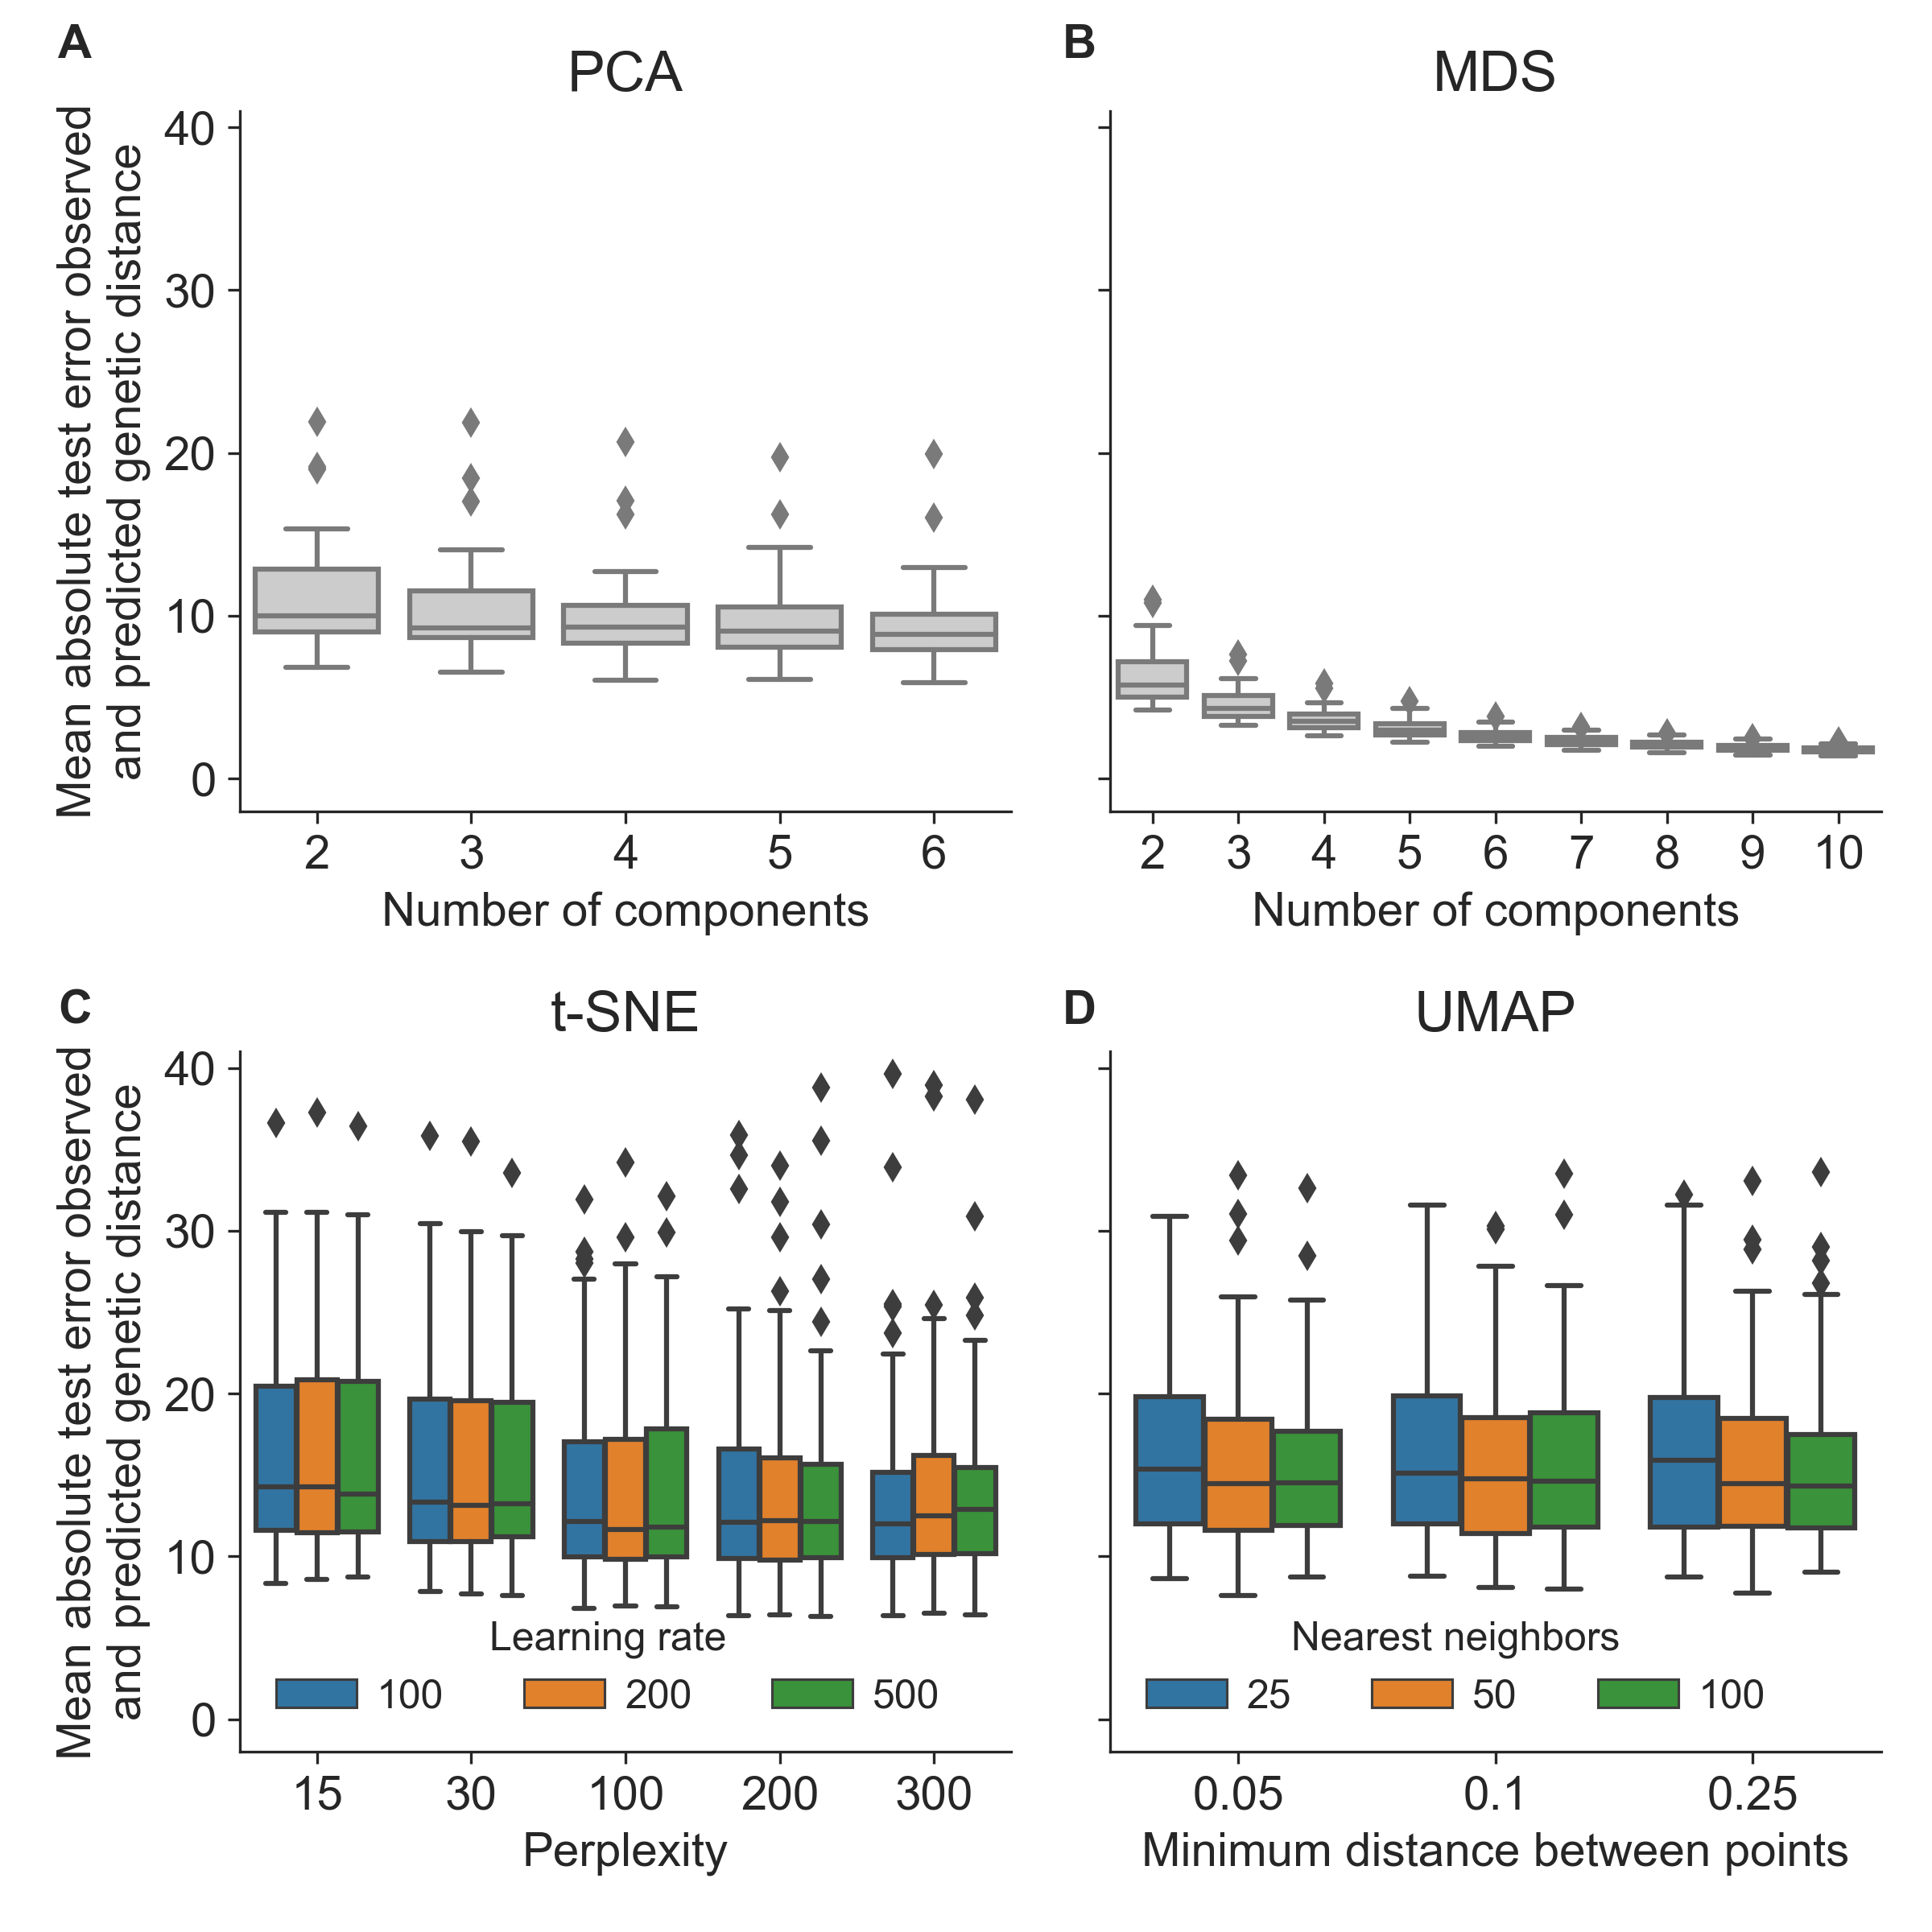
\includegraphics[width=\columnwidth]{figures/simulated-influenza-like-with-no-reassortment-scores-by-parameters.png}
  \caption*{{\bf S1 Fig. Distribution of mean absolute errors (MAE) between observed and predicted pairwise genetic distances per embedding method parameters for simulated influenza-like populations.}}
\end{figure}

The optimal parameters for coronavirus-like populations were nearly the same as those for the influenza-like populations.
The optimal parameters were 2 components for PCA, 3 for MDS, perplexity of 100 and learning rate of 500 for t-SNE, and nearest neighbors of 100 and minimum distance of 0.05 for UMAP.
As with influenza-like populations, both PCA and MDS showed diminishing benefits of increasing the number of components (\nameref{S2_Fig_simulated_coronavirus_errors} A and B).
Similarly, we observed little improvement in MAEs from varying t-SNE and UMAP parameters (\nameref{S2_Fig_simulated_coronavirus_errors} C and D).
The most noticeable improvement came from setting t-SNE's perplexity to 100 (\nameref{S2_Fig_simulated_coronavirus_errors} C).
These results indicate the limits of t-SNE and UMAP to represent global genetic structure, at least across the parameter regimes considered here.
\jhc{An obvious follow-up question would be whether we can improve MAEs for these methods by increasing components available to them, too.}

% TODO: remove supporting information figures in final submission; figures must be uploaded separately from the manuscript.
\begin{figure}[!h]
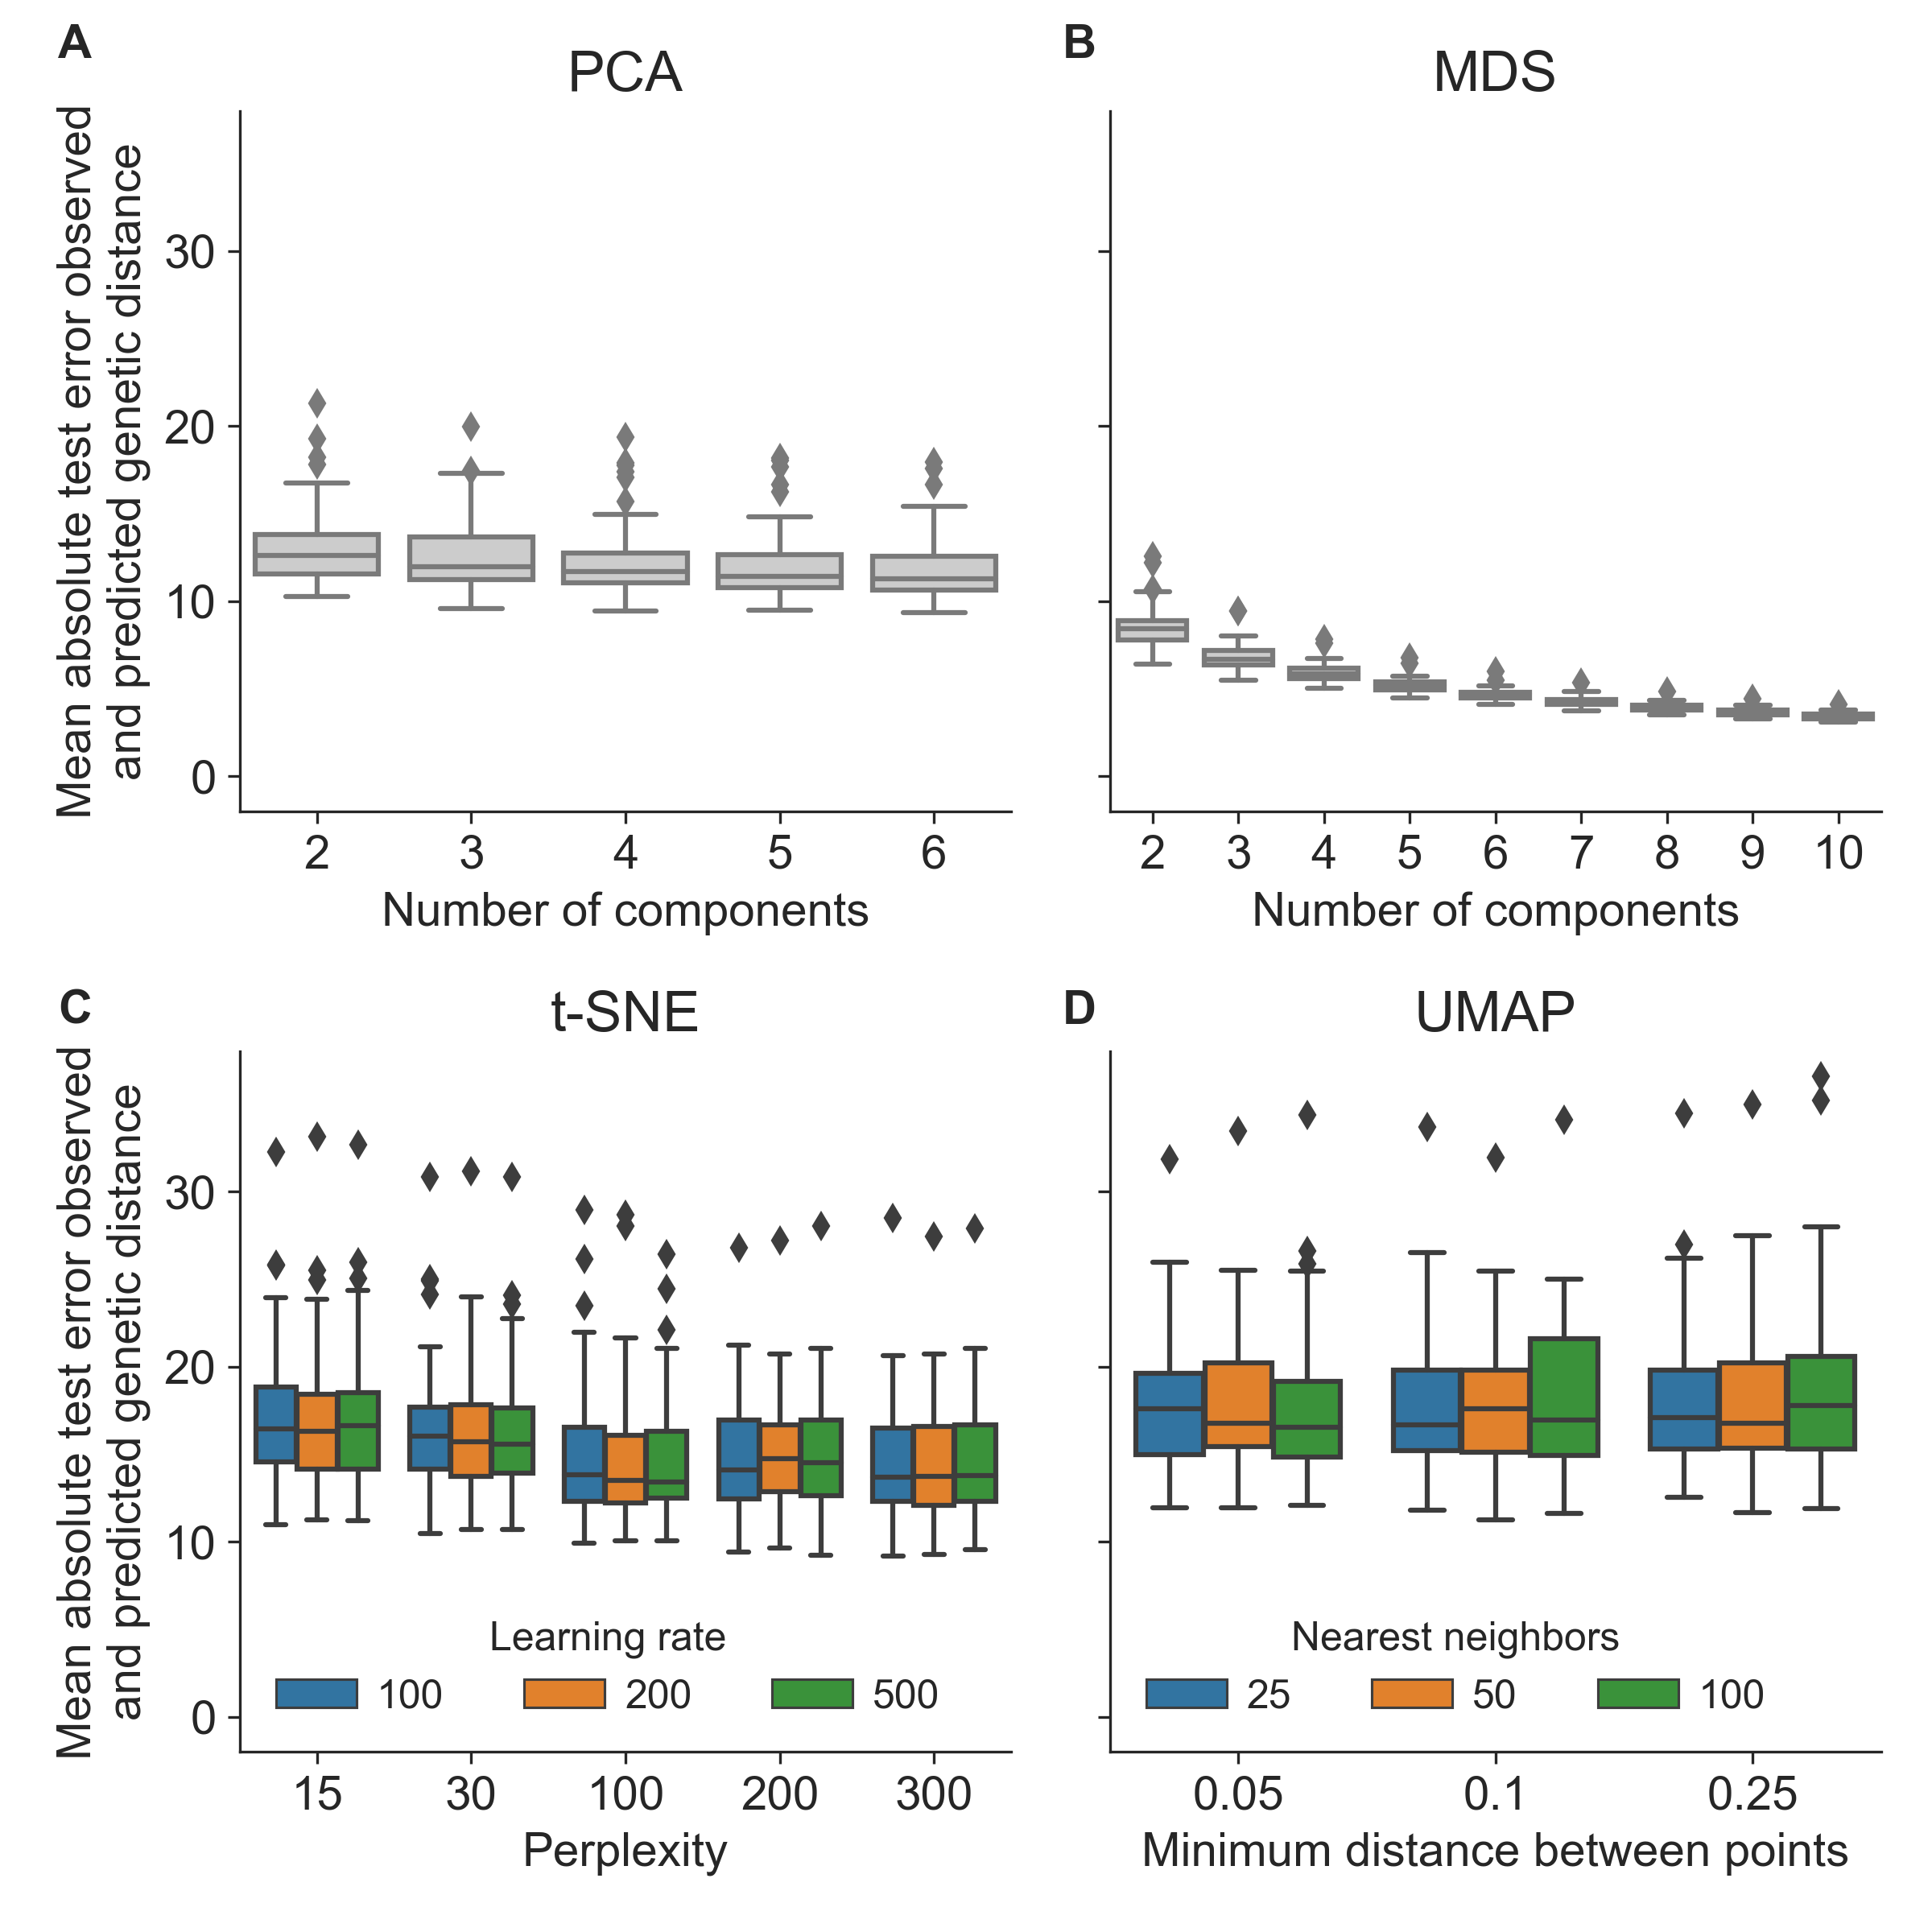
\includegraphics[width=\columnwidth]{figures/simulated-coronavirus-like-with-moderate-recombination-rate-scores-by-parameters.png}
\caption*{{\bf S2 Fig. Distribution of mean absolute errors (MAE) between observed and predicted pairwise genetic distances per embedding method parameters for simulated coronavirus-like populations.}}
\end{figure}

We inspected representative embeddings based on the optimal parameters above for the first four years of influenza- and coronavirus-like populations.
Simulated sequences collected from the same time period tended to map closer in embedding space, indicating the maintenance of ``local'' genetic structure in the embeddings (Fig.~\ref{fig:simulated-populations-representative-embeddings}).
Most embeddings also represented some form of global structure, with later generations mapping closer to intermediate generations than earlier generations.
MDS maintained the greatest continuity between generations for both population types (\nameref{S3_Fig_simulated_representative_mds_embeddings}).
In contrast, PCA, t-SNE, and UMAP all demonstrated tighter clusters of samples separated by potentially arbitrary space.
The UMAP embedding for the coronavirus-like samples was most extreme in this respect, with a tight cluster of early samples placing far away from all other samples in the embedding including those from nearby generations.
These qualitative results matched our expectations based on how well each method maximized a linear relationship between genetic and Euclidean distances during parameter optimization (\nameref{S1_Fig_simulated_flu_errors} and \nameref{S2_Fig_simulated_coronavirus_errors}).

\begin{figure}[!h]
% TODO: remove includegraphics commands in final submission; figures must be uploaded separately from the manuscript.
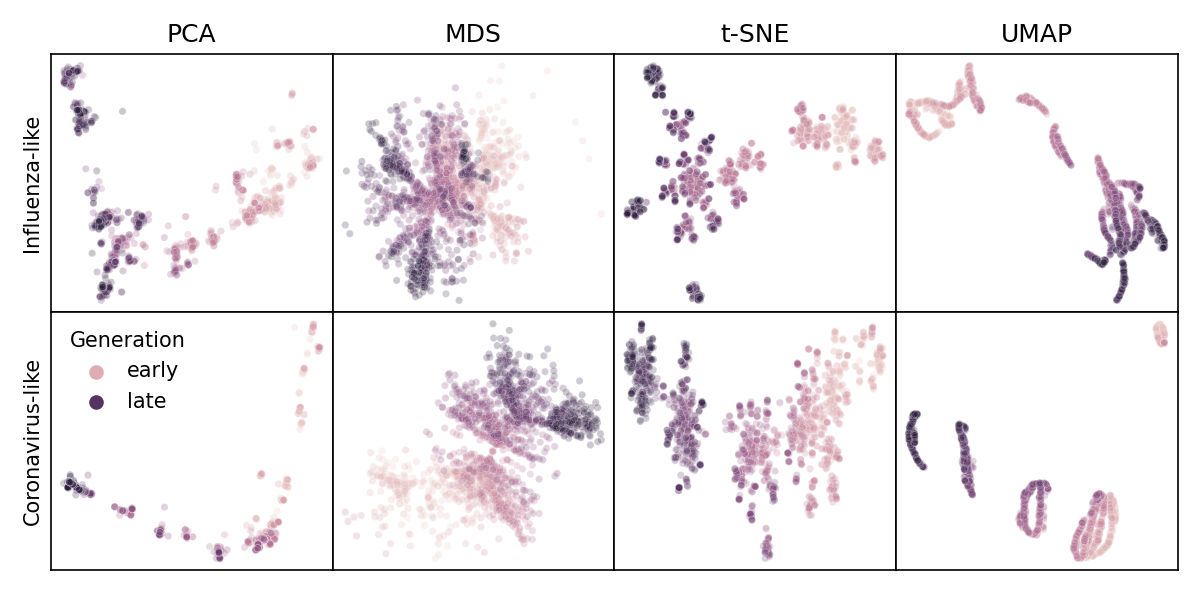
\includegraphics[width=\columnwidth]{figures/simulated-populations-representative-embeddings.png}
\caption{{\bf Representative embeddings for simulated populations using optimal parameters per pathogen (rows) and embedding method (columns).}
  Each panel shows the embedding for sequences from the first four years of a single replicate population for the corresponding pathogen type.
  Each point represents a simulated viral sequence colored by its generation with darker values representing later generations.
  The MDS embedding shows the first two of three total components.
  \nameref{S3_Fig_simulated_representative_mds_embeddings} shows the full MDS embedding for all components.}
\label{fig:simulated-populations-representative-embeddings}
\end{figure}

\begin{figure}[!h]
% TODO: remove includegraphics commands in final submission; figures must be uploaded separately from the manuscript.
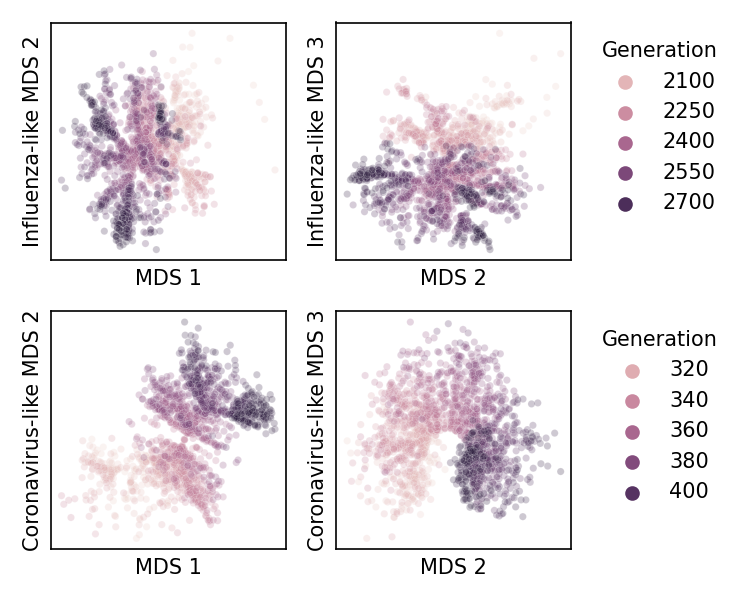
\includegraphics[width=\columnwidth]{figures/simulated-populations-representative-mds-embeddings.png}
\caption*{{\bf S3 Fig. Representative MDS embeddings for simulated populations using optimal parameters per pathogen (rows) and showing all three components.}}
\end{figure}

\subsection*{Embedding clusters recapitulate phylogenetic clades for seasonal influenza H3N2}

Seasonal influenza H3N2's hemagglutinin (HA) sequences provide an ideal positive control to test embedding methods and clustering in low-dimensional space.
H3N2's HA protein evolves rapidly, accumulating amino acid mutations that enable escape from adaptive immunity in human populations \cite{Petrova2018}.
These mutations produce distinct phylogenetic clades that represent potentially different antigenic phenotypes.
The World Health Organization (WHO) Global Influenza Surveillance and Response System (GISRS) regularly sequences genomes of circulating influenza lineages \cite{Hay2018} and submits these sequences to public INSDC databases like NCBI's GenBank \cite{Arita2021}.
These factors, coupled with HA's relatively short gene size of 1,701 nucleotides, facilitate real-time genomic epidemiology of H3N2 \cite{Neher2015} and rapid analysis by the embedding methods we wanted to evaluate.

We first applied each embedding method to the early H3N2 HA sequences collected from 2016 through 2018, colored samples by previously defined phylogenetic clades, and inspected the placement of these samples in the embeddings and corresponding phylogeny.
All four embedding methods qualitatively recapitulated clade-level groupings observed in the phylogeny (Fig~\ref{fig:seasonal-influenza-h3n2-ha-embeddings}).
Samples from the same clade generally grouped tightly together.
Most embedding methods also clearly delineated larger phylogenetic clades, placing clades A1, A2, A3, A4, and 3c3.A into separate locations in the embeddings.
One exception to this pattern was the PCA embedding which grouped samples from clades A3 and A4 into the same space.
Despite maintaining local and broader global structure, not all embeddings captured intermediate genetic structure.
For example, clade A1b descended from clade A1 and diversified into the smaller subclades A1b/131K, A1b/135K, and A1b/135N.
All methods placed A1b far from its ancestor A1, but all methods also placed descendants of A1b into tight clusters together.
The t-SNE embedding created separate clusters of the three descendant clades, but these clusters all placed so close together in the embedding space that, without previously defined clade labels, we would have visually grouped these samples into a single cluster.
These results qualitatively replicate the patterns we observed in embeddings for simulated influenza-like populations (Fig~\ref{fig:simulated-populations-representative-embeddings}).

% For figure citations, please use "Fig" instead of "Figure".

% Place figure captions after the first paragraph in which they are cited.
\begin{figure}[!h]
% TODO: remove includegraphics commands in final submission; figures must be uploaded separately from the manuscript.
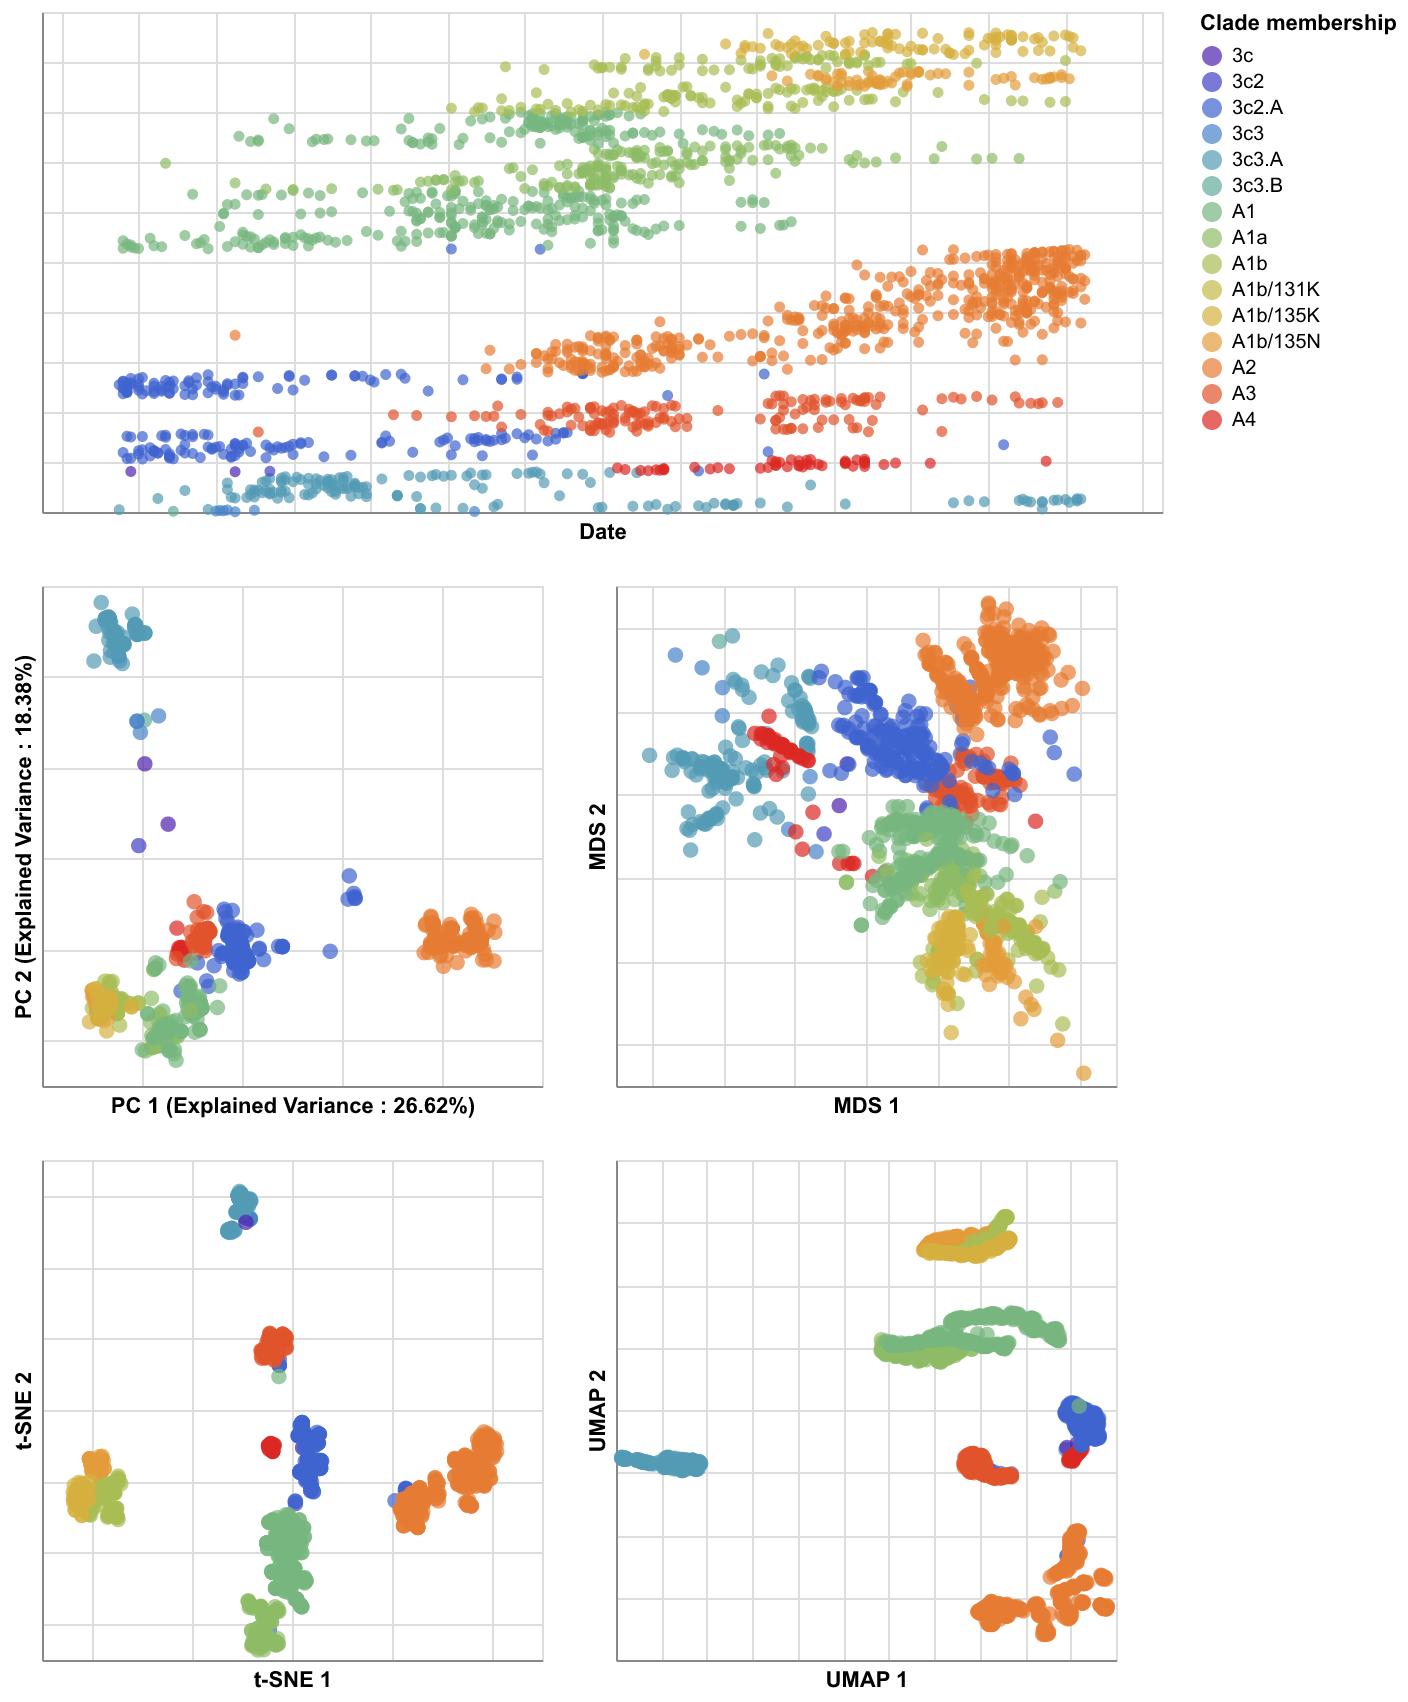
\includegraphics[width=\columnwidth]{figures/flu-2016-2018-ha-embeddings-by-clade.png}
\caption{{\bf Phylogeny of early (2016--2018) influenza H3N2 HA sequences (top) and low-dimensional embeddings of the same sequences by PCA (middle left), MDS (middle right), t-SNE (bottom left), and UMAP (bottom right).}
}
\label{fig:seasonal-influenza-h3n2-ha-embeddings}
\end{figure}

To quantify the apparent maintenance of local and global structure by all four embedding methods, we calculated the relationship between pairwise genetic and Euclidean distance of samples in each embedding.
All four methods maintained a linear relationship between genetic and Euclidean distances for samples that differed by no more than $\approx$10 nucleotides (Fig~\ref{fig:seasonal-influenza-h3n2-ha-pairwise-distances}).
However, only MDS consistently maintained that linearity as genetic distance increased (Pearson's $R^{2} = 0.94$).
Values of Euclidean distances in MDS corresponded nearly perfectly with values of genetic distances.
In contrast, we observed a nonlinear relationship for samples with more genetic differences in PCA (Pearson's $R^{2} = 0.67$), t-SNE (Pearson's $R^{2} = 0.37$), and UMAP (Pearson's $R^{2} = 0.48$) embeddings.
Although the most genetically distant samples mapped far from each other in all of these embeddings, samples with intermediate distances could map much closer or farther than expected by a linear model.
In t-SNE and UMAP embeddings, some pairs of samples with intermediate distances of 30-40 nucleotides mapped farther apart than pairs of samples with much greater genetic distances.

\begin{figure}[!h]
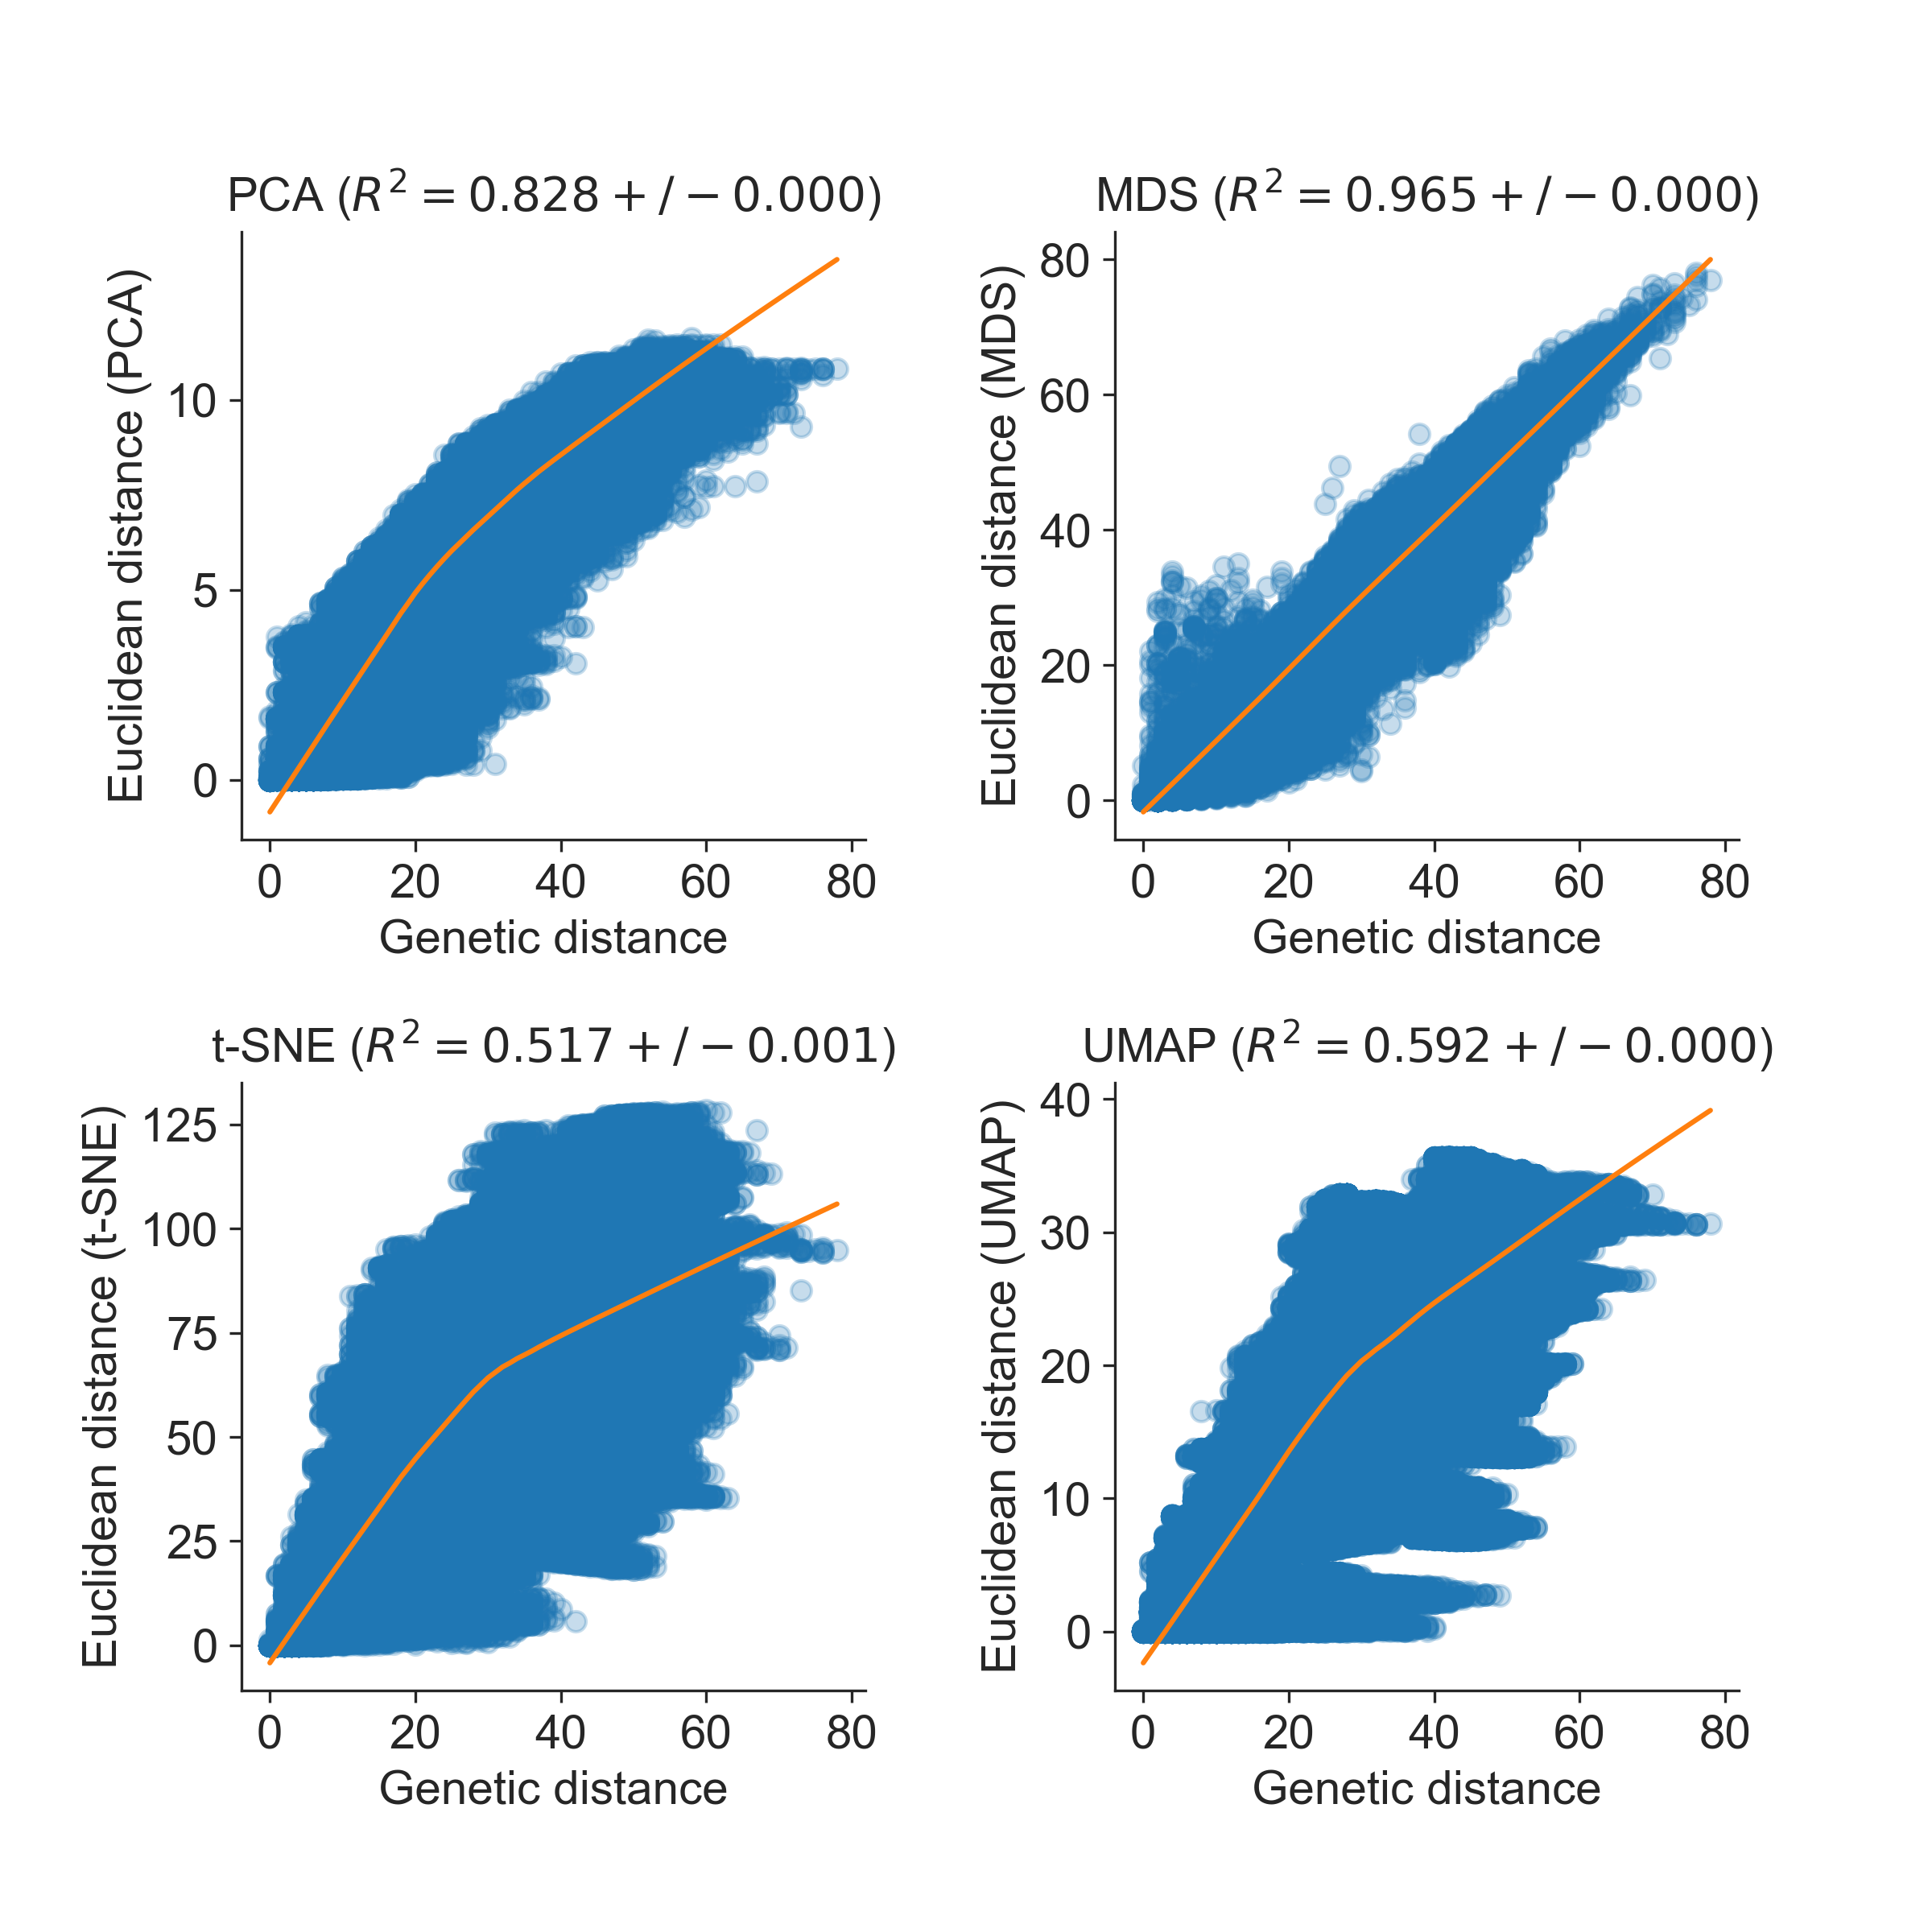
\includegraphics[width=\columnwidth]{figures/flu-2016-2018-ha-euclidean-distance-by-genetic-distance.png}
\caption{{\bf Relationship between pairwise genetic and Euclidean distances in embeddings of early (2016--2018) influenza H3N2 HA sequences by PCA (upper left), MDS (upper right), t-SNE (lower left), and UMAP (lower right)}}
\label{fig:seasonal-influenza-h3n2-ha-pairwise-distances}
\end{figure}

Next, we measured how well clusters of H3N2 HA samples in each embedding corresponded to previously defined genetic groups.
For each embedding, we assigned cluster labels to each sample with the hierarchical clustering algorithm, HDBSCAN, which does not require an expected number of clusters as input \cite{campello2015hierarchical}.
HDBSCAN does require definition of a minimum distance that its initial clusters must be from each other to avoid being merged into the same cluster.
This distance corresponds to the Euclidean distance between clusters in embedding space which varies by method (Fig~\ref{fig:seasonal-influenza-h3n2-ha-pairwise-distances}).
To find the optimal minimum distance for HDBSCAN clusters of H3N2 HA data, we assigned clusters to each embedding for a range of distance values (0-7) with a step size of 0.5 and calculated the accuracy of clusters at each distance value compared to the Nextstrain clade assignments shown in Fig~\ref{fig:seasonal-influenza-h3n2-ha-embeddings}.
We selected the minimum distance value per method that minimized the difference between HDBSCAN clusters and clade assignments as measured by the normalized variation of information (VI) metric \cite{meilua2003comparing} (see Methods).
The optimal minimum distances were 0.5 for PCA, 3.5 for MDS, 2.0 for t-SNE, and 1.0 for UMAP (Table~\ref{table:accuracy}).
Since Euclidean distances for MDS correspond directly to genetic distances, these results show that clusters must be at least 3.5 nucleotides apart to be considered distinct.

% Place tables after the first paragraph in which they are cited.
\begin{table}[!ht]
%\begin{adjustwidth}{-2.25in}{0in} % Comment out/remove adjustwidth environment if table fits in text column.
\centering
\caption{
  {\bf Accuracy of embedding methods per human pathogenic virus sorted by normalized variation of information (VI) distance.}
  Smaller VI values indicate smaller distances between HDBSCAN clusters and known genetic groups with 0 indicating identical clusters and 1 indicating maximally different clusters.
  Threshold refers to the distance threshold used to assign clusters with HDBSCAN.}
\begin{tabular}{llrr}
\toprule
                     Pathogen & Method &   VI &  Threshold \\
\midrule
               Influenza H3N2 &  t-SNE & 0.04 &        2.0 \\
                              &   UMAP & 0.08 &        1.0 \\
                              &    MDS & 0.10 &        3.5 \\
                              &    PCA & 0.19 &        0.5 \\
SARS-CoV-2 (Nextstrain clade) &  t-SNE & 0.07 &        1.0 \\
                              &    MDS & 0.15 &        0.0 \\
                              &   UMAP & 0.16 &        0.5 \\
                              &    PCA & 0.22 &        0.5 \\
           SARS-CoV-2 (Pango) &  t-SNE & 0.12 &        1.0 \\
                              &    MDS & 0.23 &        0.0 \\
                              &   UMAP & 0.25 &        0.5 \\
                              &    PCA & 0.31 &        0.5 \\
\bottomrule
\end{tabular}

\label{table:accuracy}
%\end{adjustwidth}
\end{table}

As expected, the clusters for each method generally corresponded to larger phylogenetic clades (Fig~\ref{fig:seasonal-influenza-h3n2-ha-2016-2018-clusters}).
Clusters from t-SNE most accurately captured expert clade assignments (normalized VI=0.04) with nine clusters.
These clusters captured broader phylogenetic clades (A1, A1b, A2, A3, A4, 3c2.A, and 3c3.A) but failed to distinguish between A1b and its descendants.
Clusters from UMAP performed nearly as well (normalized VI=0.08) with six clusters.
These clusters captured broader clades, but they failed to distinguish among A1 and A1a, A1b and its subclades, and 3c2.A and A4.
The nine MDS clusters were more than twice as far from expert clades as t-SNE clusters (normalized VI=0.10), but this difference in accuracy appeared to be driven primarily by the cost of more samples that HDBSCAN failed to assign to clusters in the MDS embedding.
MDS clusters captured most of the larger clades (A1, A2, A3, A4, 3c2.A, and 3c3.A), but they also collected A1 and its descendants into two large clusters.
The PCA embedding produced the lowest accuracy (normalized VI=0.19) and fewest clusters (N=3).
PCA's three clusters corresponded to some of the most distantly-related and ancestral clades (3c2.A, 3c3.A, and A2).
We identified 30 cluster-specific mutations for all three PCA clusters, 34 for seven of the nine MDS clusters, 32 for six of nine t-SNE clusters, and 25 for four of the six UMAP clusters (\nameref{S1_Table}).
We also found that pairwise genetic distances between sequences in the same MDS, t-SNE, or UMAP clusters matched the genetic distances between sequences in the same Nextstrain clades (\nameref{S4_Fig_flu_within_between_group_distances}).
These results indicate that nonlinear embeddings of t-SNE and UMAP could be better-suited for clustering and classification than linear embeddings from PCA and MDS.

\begin{figure}[!h]
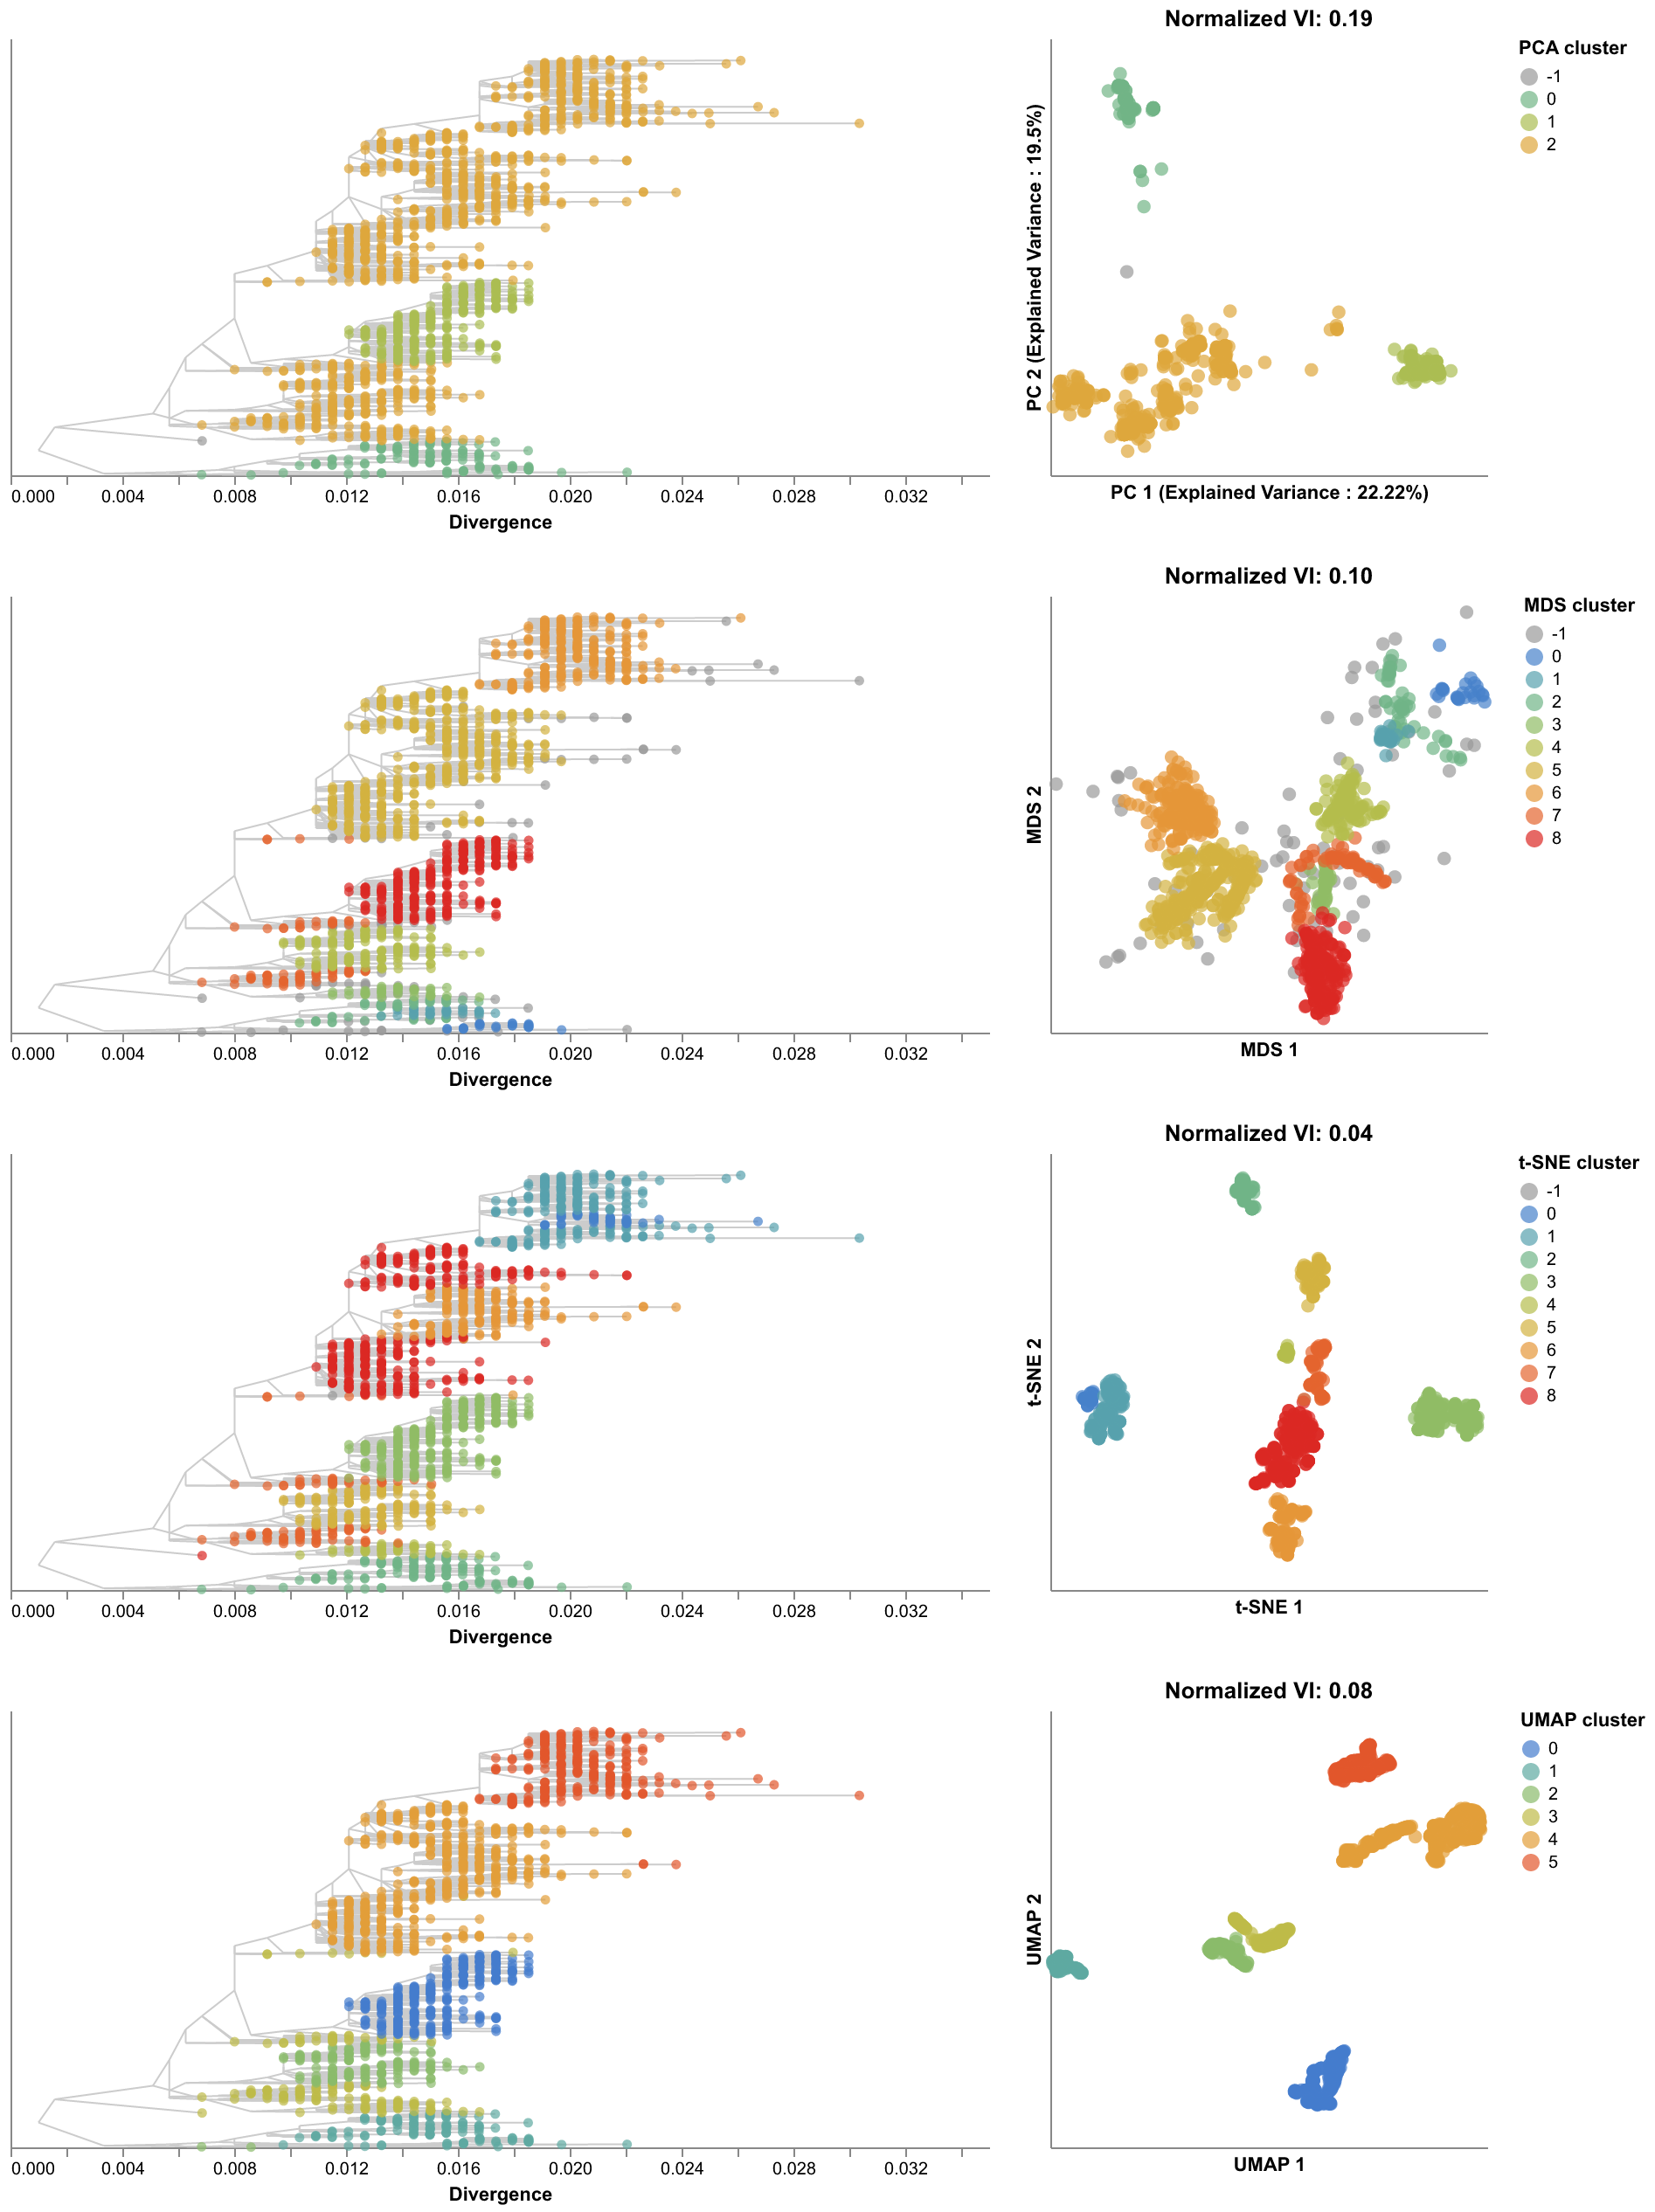
\includegraphics[width=\columnwidth]{figures/flu-2016-2018-ha-embeddings-by-cluster.png}
\caption{{\bf Phylogenetic trees (left) and embeddings (right) of early (2016--2018) H3N2 HA sequences colored by HDBSCAN cluster.}
Normalized VI values per embedding reflect the distance between clusters and known genetic groups (Nextstrain clades).}
\label{fig:seasonal-influenza-h3n2-ha-2016-2018-clusters}
\end{figure}

\begin{figure}[!h]
% TODO: remove includegraphics commands in final submission; figures must be uploaded separately from the manuscript.
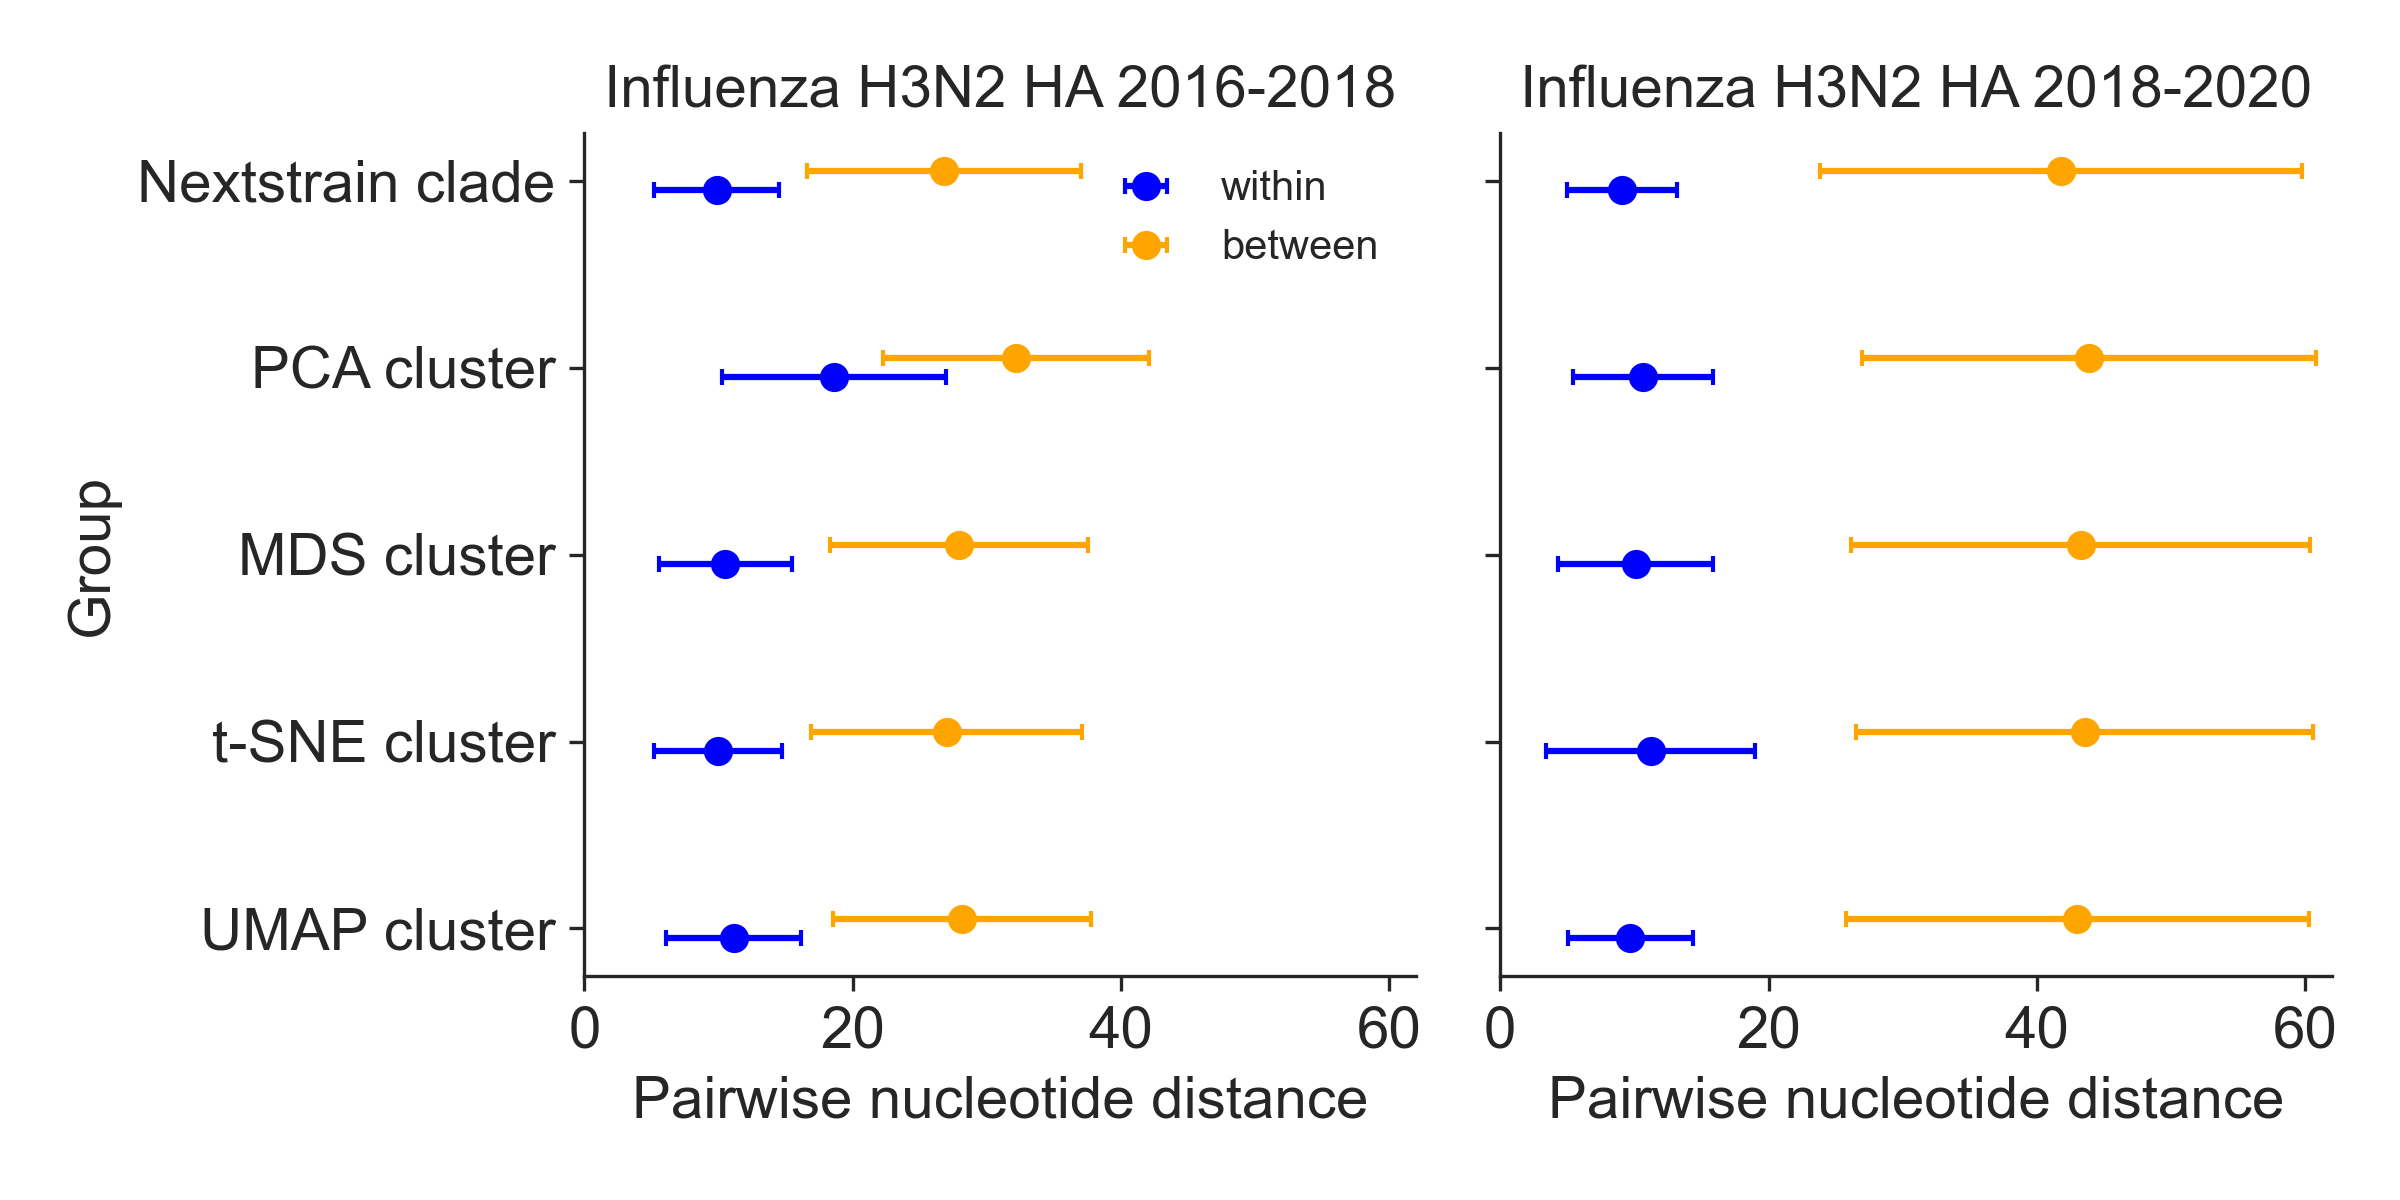
\includegraphics[width=\columnwidth]{figures/within_between_influenza.png}
\caption*{{\bf S4 Fig. Pairwise nucleotide distances for early (2016--2018) and late (2018--2020) influenza H3N2 HA sequences within and between genetic groups defined by Nextstrain clades and clusters from PCA, MDS, t-SNE, and UMAP embeddings.}}
\end{figure}

To understand whether these embedding methods and optimal cluster parameters could effectively cluster previously unseen sequences, we applied each method to the late H3N2 HA dataset (2018--2020), clustered sequences in the embedding space with HDBSCAN using the optimal minimum distance threshold from the early dataset, and calculated the accuracy of the cluster assignments based on previously defined clades.
Unlike the early H3N2 HA dataset, the late dataset represented less genetic diversity with most clades descending from clade A1b with at least one additional characteristic HA1 amino acid substitution (\nameref{S5_Fig_late_flu_embeddings_by_clade}).
The tree also included older samples from clades A2 and 3c3.A.
Clusters from all four methods generally captured relevant phylogenetic clades (Fig.~\ref{fig:seasonal-influenza-h3n2-ha-2018-2020-clusters} and \nameref{S5_Fig_late_flu_embeddings_by_clade}).
The MDS clusters most accurately captured expert clades (normalized VI=0.06) with 8 clusters corresponding to clades 3c3.A, A2, A3, A1b/94N, A1b/135K, A1b/135N, A1b/137F, and A1b/131K merged with A1b/197R (Fig.~\ref{fig:seasonal-influenza-h3n2-ha-2018-2020-clusters} and \nameref{S6_Fig_late_flu_mds_embeddings}).
Similarly, MDS cluster 4 merged a separate subset of A1b/131K samples with their descendants in A1b/94N.
MDS failed to create a cluster for A1b/186D samples, leaving these all as unassigned.
Both t-SNE and UMAP followed closely in accuracy (normalized VI=0.09) with 6 and 5 clusters, respectively.
Both sets of clusters generally matched those from MDS except that the most recent clades clustered into broader groups with their ancestral clades (e.g., A1b/135K and A1b/131K).
PCA produced clusters with the lowest accuracy (normalized VI=0.11), but these 6 clusters were not qualitatively much different from t-SNE and UMAP clusters.
PCA clusters split clade 3c3.A into two groups and merged A1b/94N with a larger cluster of its ancestral clade, A1b/131K, and that ancestor's other descendants.
We identified 58 cluster-specific mutations for three of the six PCA clusters, 43 for seven of the eight MDS clusters, 54 for all six t-SNE clusters, and 49 for four of the five UMAP clusters (\nameref{S1_Table}).
Pairwise genetic distances within clusters generally matched the diversity within Nextstrain clades (\nameref{S4_Fig_flu_within_between_group_distances}).
Cluster accuracies remained robust to sampling density and composition (\nameref{S7_Fig_late_flu_replication_of_cluster_accuracy}).
These results show that all four methods can produce well-supported clusters that accurately capture known genetic groups when applied to previously unseen H3N2 HA samples.

\begin{figure}[!h]
% TODO: remove includegraphics commands in final submission; figures must be uploaded separately from the manuscript.
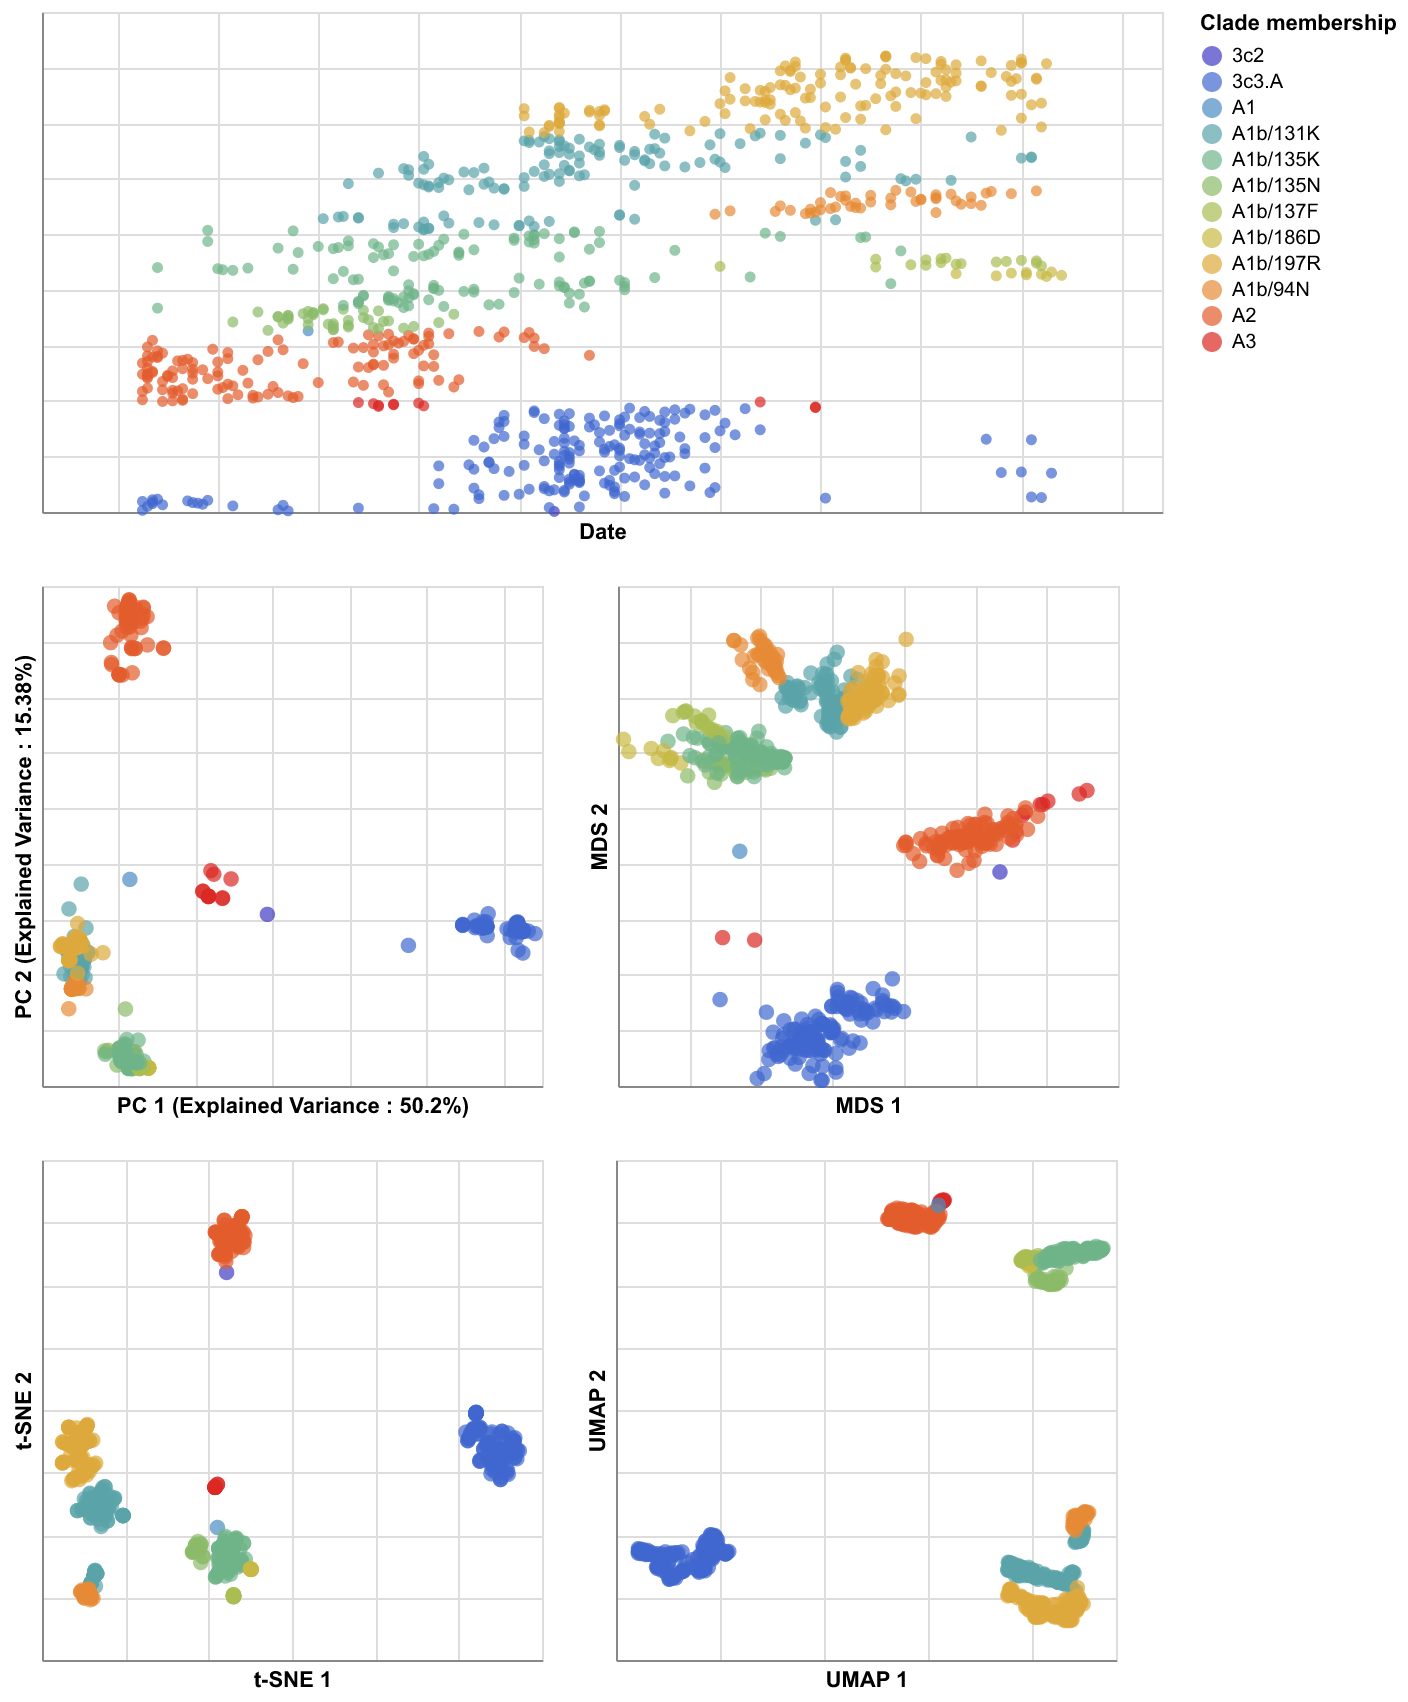
\includegraphics[width=\columnwidth]{figures/flu-2018-2020-ha-embeddings-by-clade.png}
\caption*{{\bf S5 Fig. Phylogeny of late (2018--2020) influenza H3N2 HA sequences (top) and reduced dimensionality embeddings of genetic sequences into two dimensions by PCA (middle left), MDS (middle right), t-SNE (bottom left), and UMAP (bottom right).}}
\end{figure}

\begin{figure}[!h]
% TODO: remove includegraphics commands in final submission; figures must be uploaded separately from the manuscript.
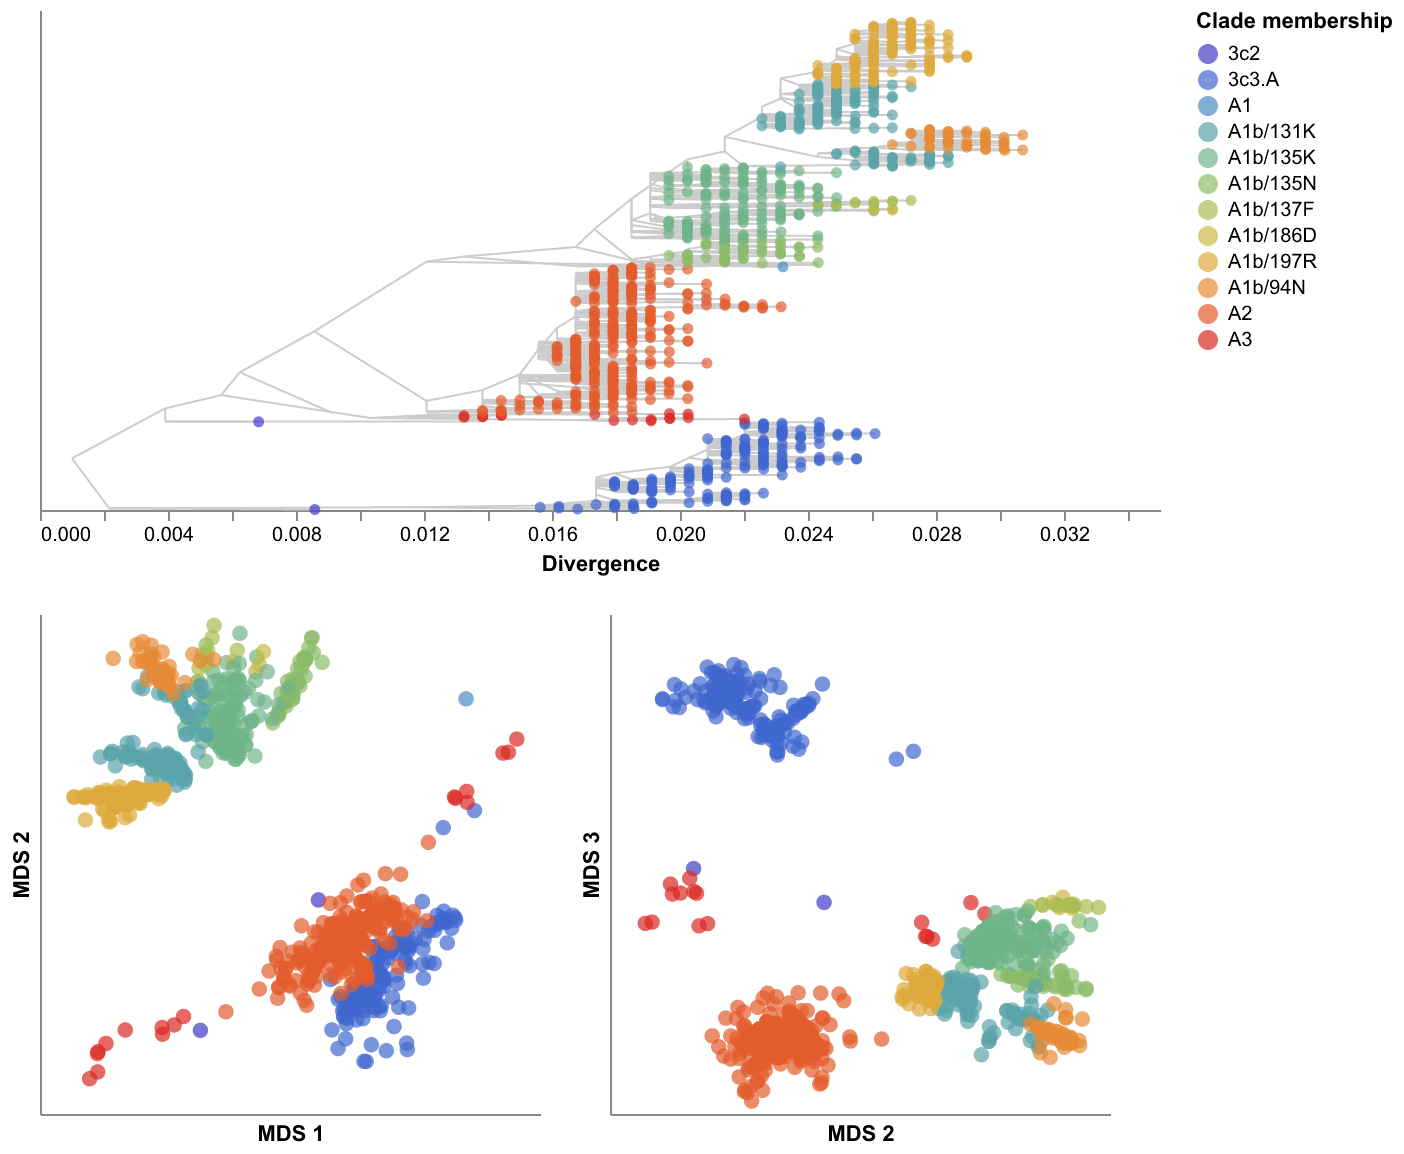
\includegraphics[width=\columnwidth]{figures/flu-2018-2020-mds-by-clade.png}
\caption*{{\bf S6 Fig. MDS embeddings for late (2018--2020) influenza H3N2 HA sequences showing all three components.}}
\end{figure}

\begin{figure}[!h]
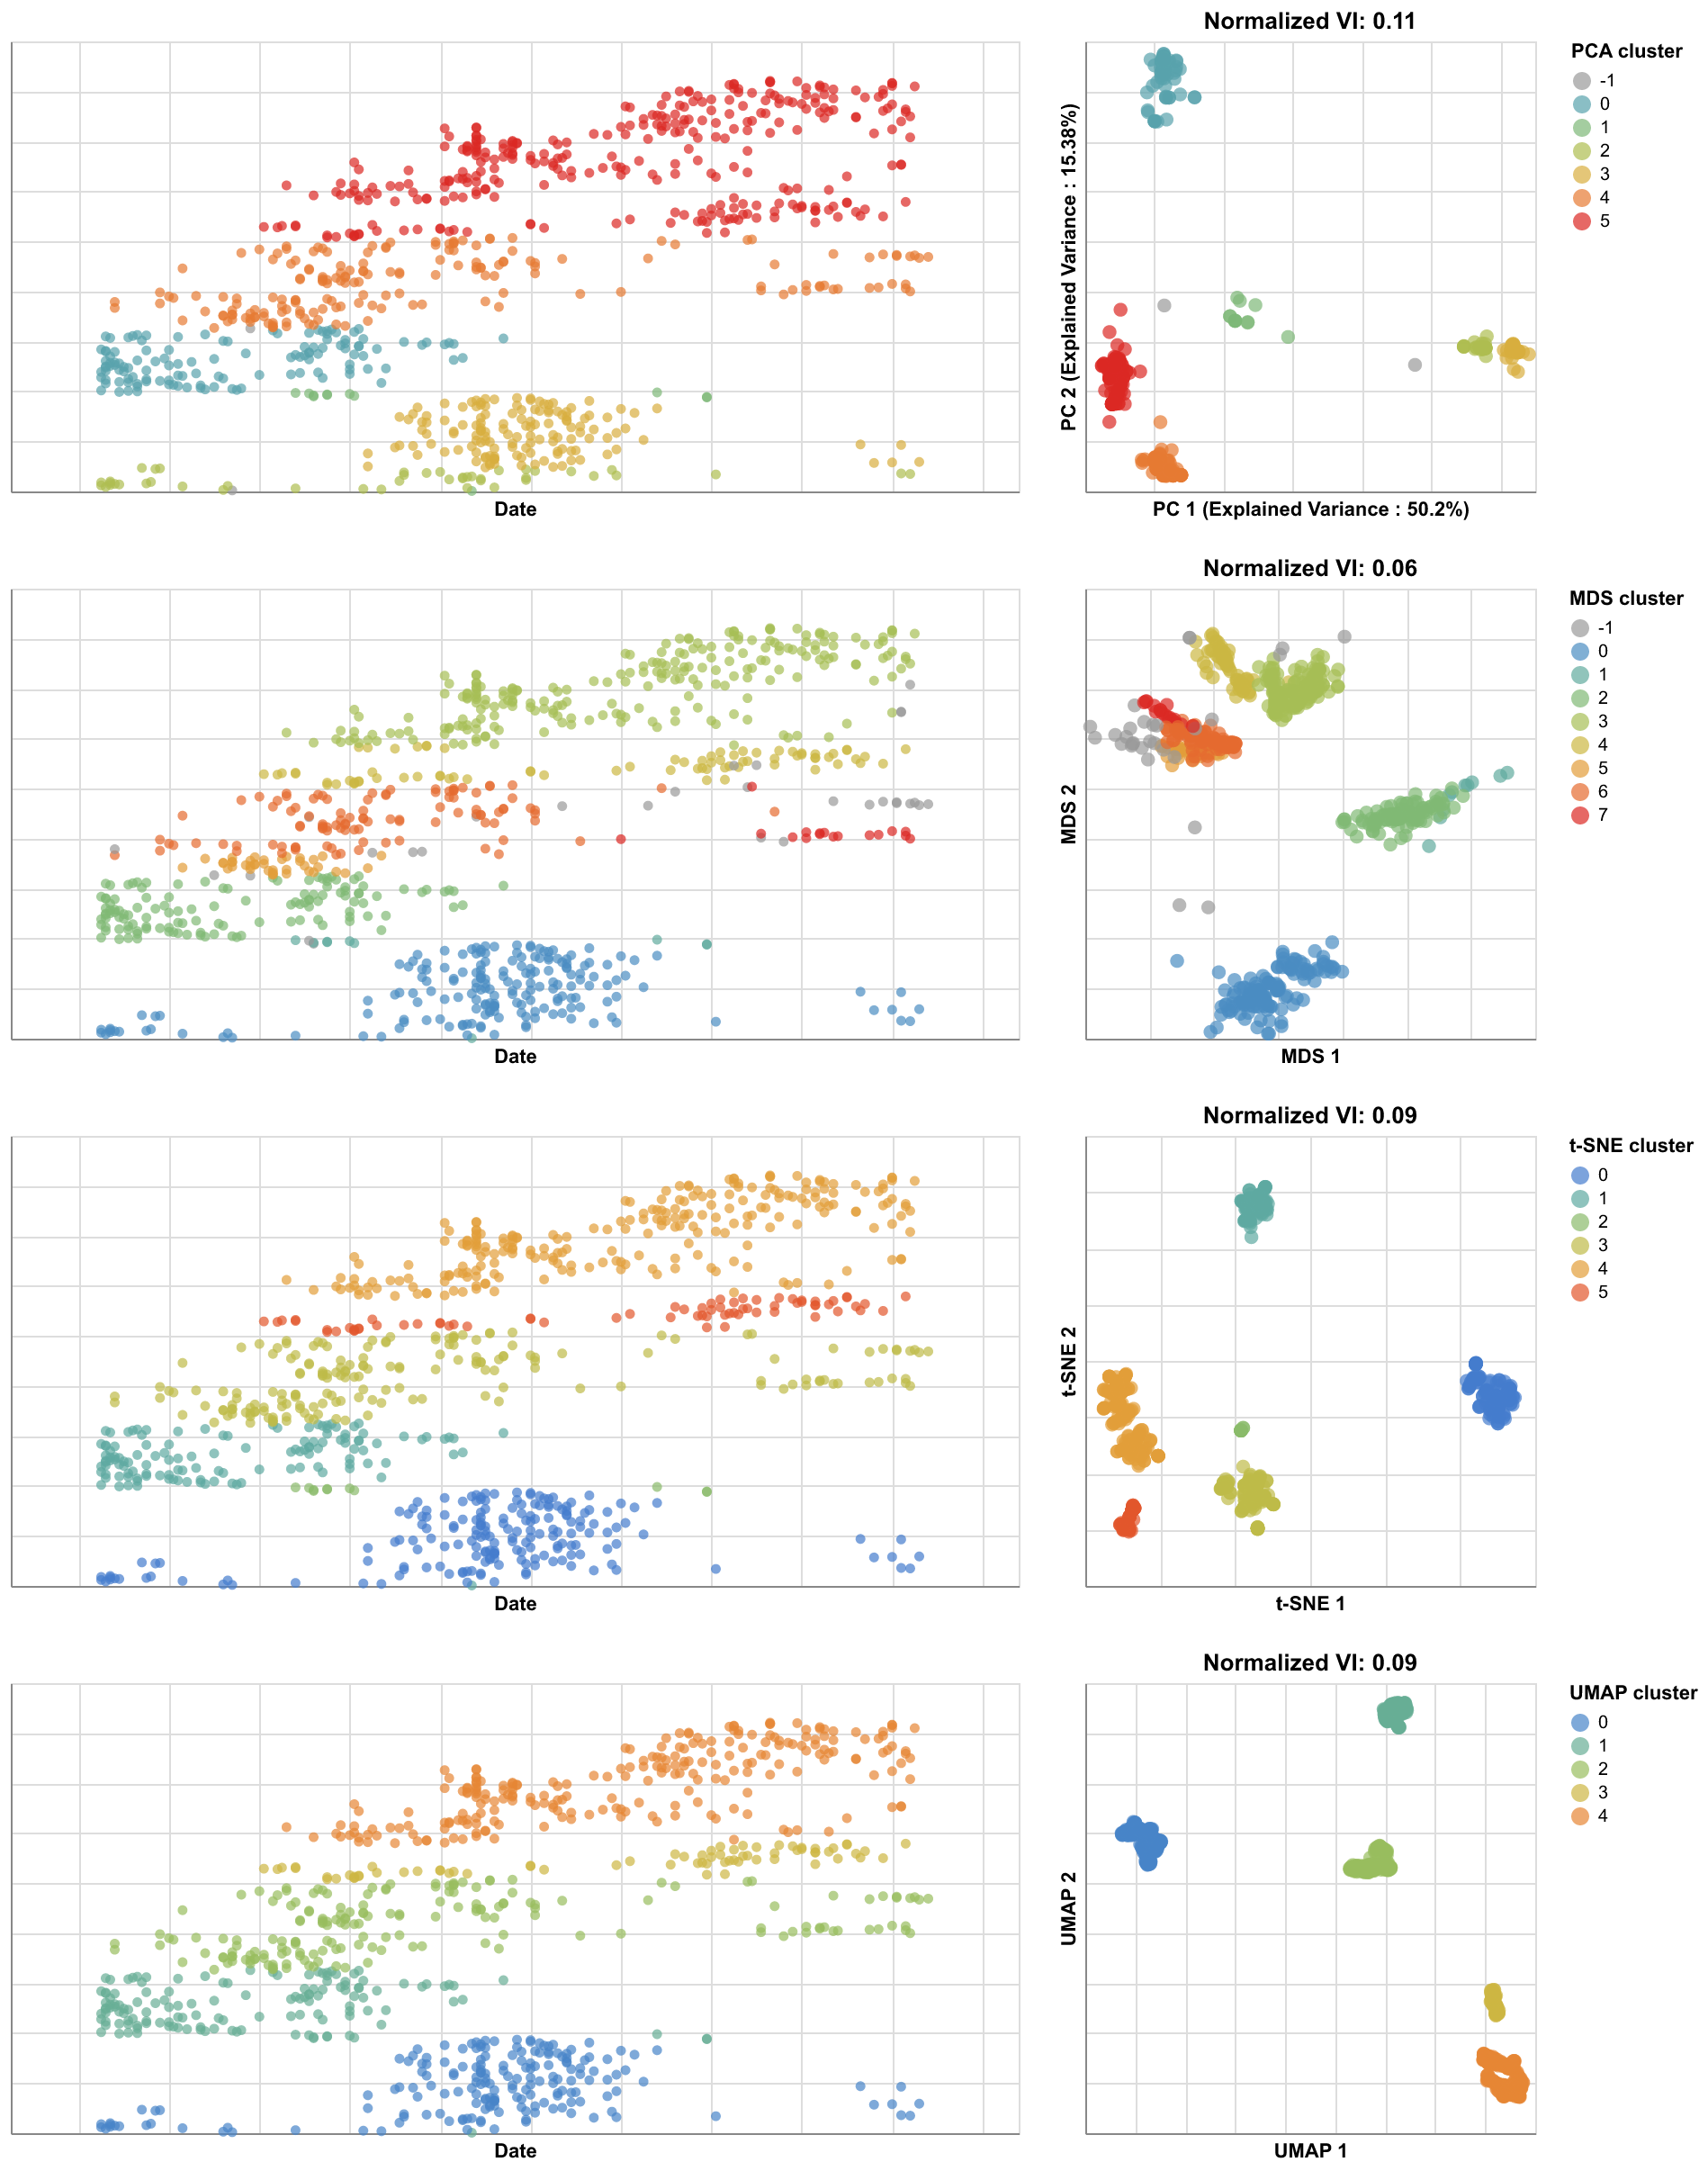
\includegraphics[width=\columnwidth]{figures/flu-2018-2020-ha-embeddings-by-cluster.png}
\caption{{\bf Phylogenetic trees (left) and embeddings (right) of late (2018--2020) H3N2 HA sequences colored by HDBSCAN cluster.}
Normalized VI values per embedding reflect the distance between clusters and known genetic groups (Nextstrain clades).}
\label{fig:seasonal-influenza-h3n2-ha-2018-2020-clusters}
\end{figure}

\begin{figure}[!h]
% TODO: remove includegraphics commands in final submission; figures must be uploaded separately from the manuscript.
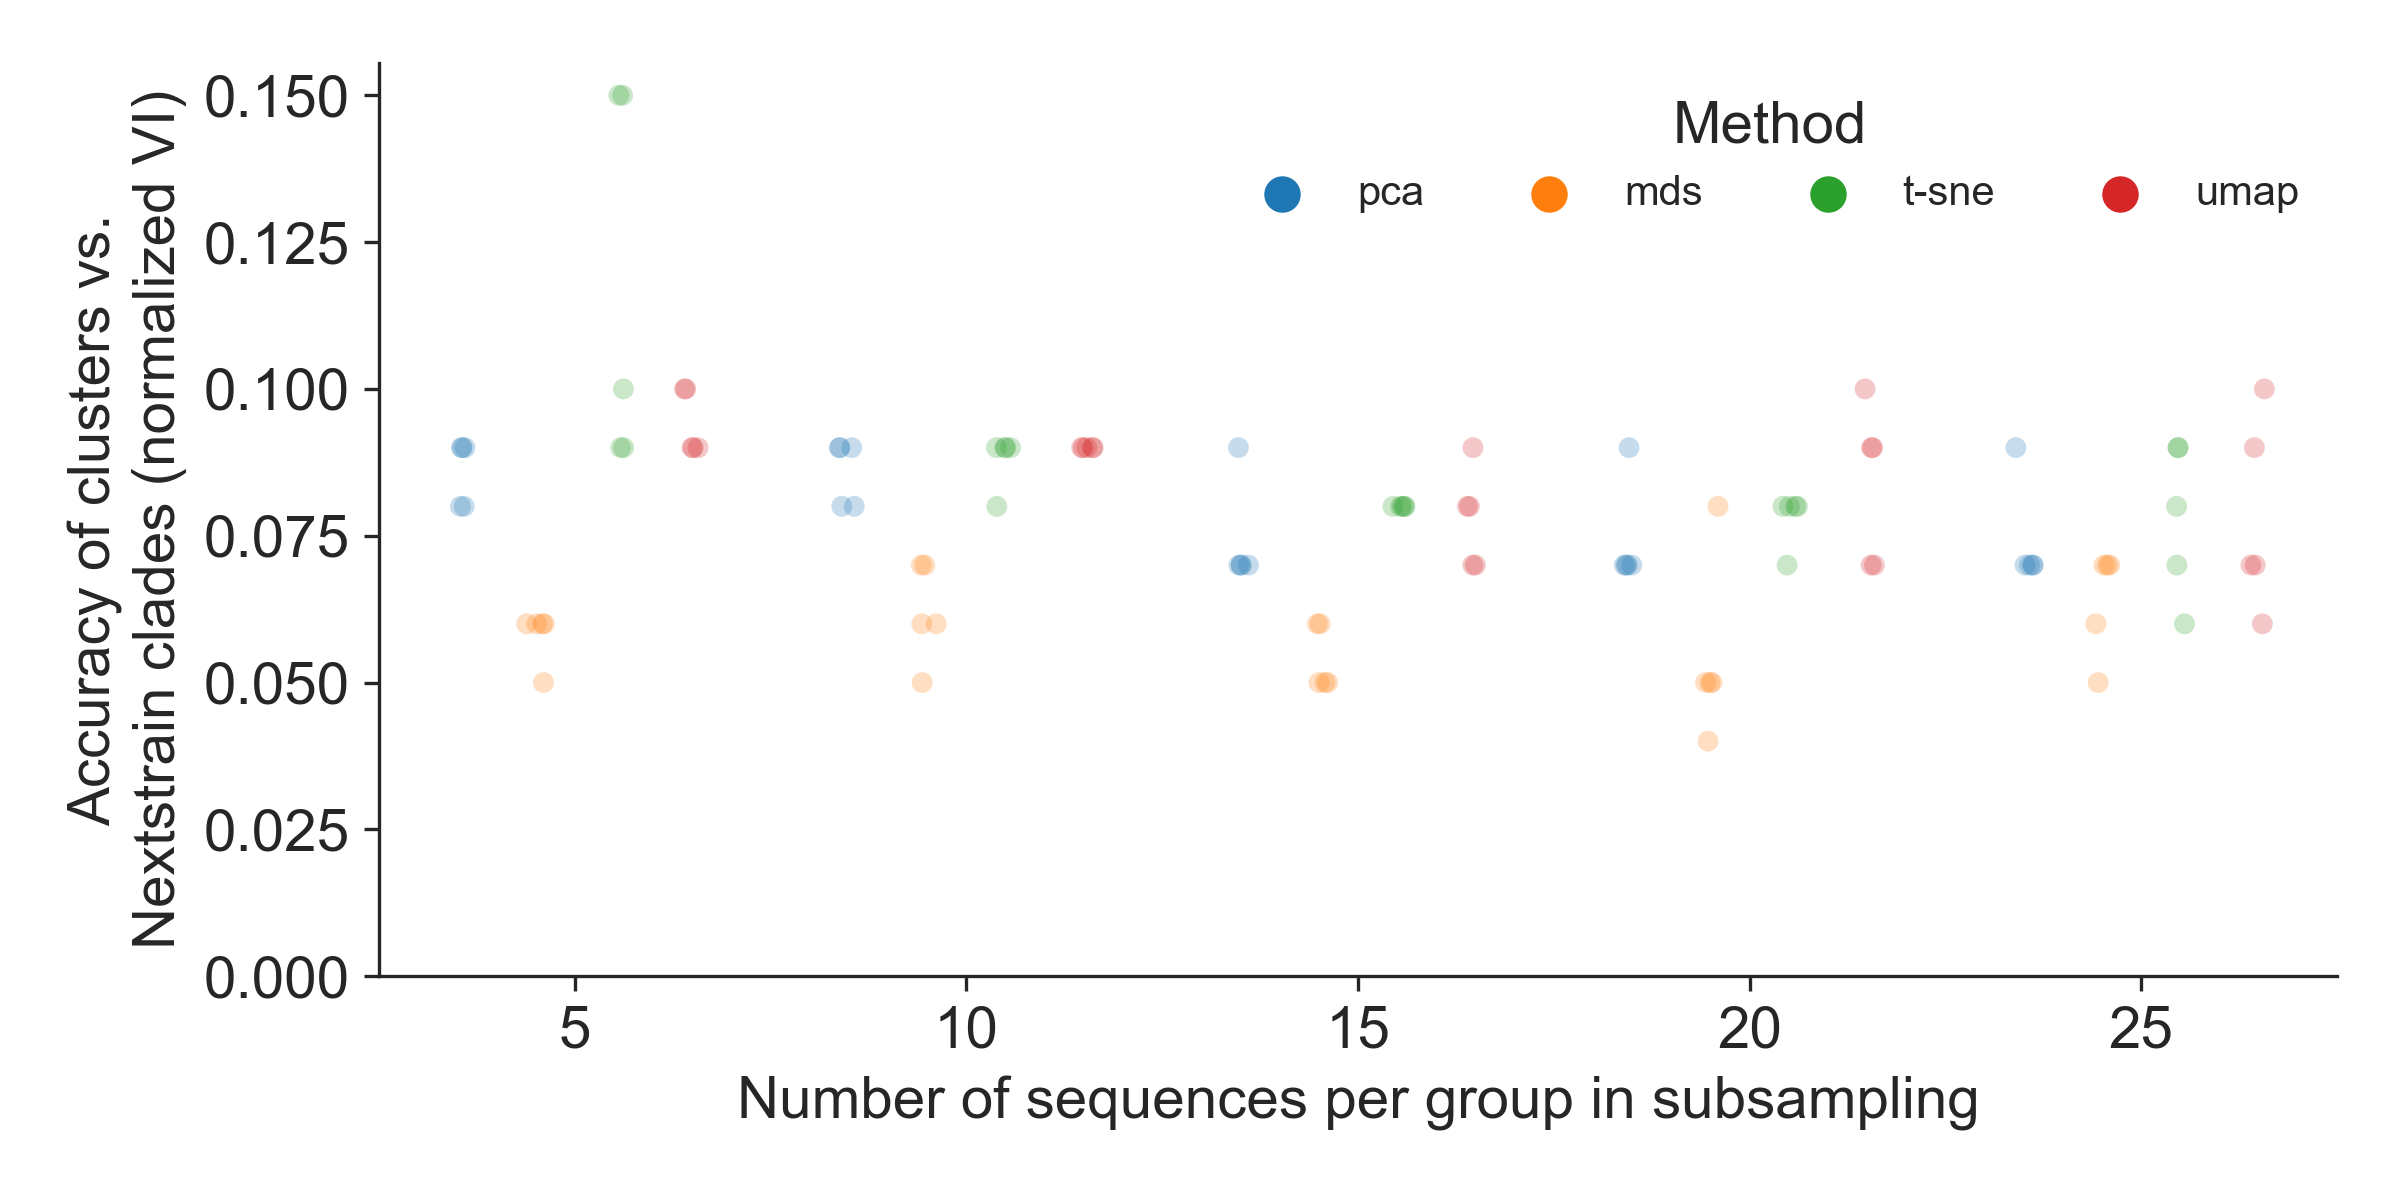
\includegraphics[width=\columnwidth]{figures/flu-2018-2020-replication-of-cluster-accuracy.png}
\caption*{{\bf S7 Fig. Replication of cluster accuracy per embedding method for late (2018--2020) influenza H3N2 HA sequences across different sequences per group sampled from the original dataset and five replicates per sampling density.}}
\end{figure}

\subsection*{Joint embeddings of hemagglutinin and neuraminidase genomes identify seasonal influenza virus H3N2 reassortment events}

Given that clusters from embedding methods could recapitulate expert-defined clades, we measured how well the same methods could capture reassortment events between multiple gene segments as detected by biologically-informed computational models.
Evolution of HA and NA surface proteins contributes to the ability of influenza viruses to escape existing immunity \cite{Petrova2018} and HA and NA genes frequently reassort \cite{Nelson2008,Marshall2013,Potter2019}.
Therefore, we focused our reassortment analysis on HA and NA sequences, sampling 1,643 viruses collected between January 2016 and October 2018 with sequences for both genes.
We aligned these sequences to a common reference (A/Beijing/32/1992), inferred HA and NA phylogenies, and applied TreeKnit to both trees to identify maximally compatible clades (MCCs) that represent reassortment events \cite{Barrat-Charlaix2022}.
Of the 206 reassortment events identified by TreeKnit, 13 (6\%) contained at least 10 samples representing 778 samples (47\%).

We created PCA, MDS, t-SNE, and UMAP embeddings from the HA alignments and from merged HA and NA alignments.
We identified clusters in both HA-only and HA/NA embeddings and calculated the VI distance between these clusters and the MCCs identified by TreeKnit.
We expected that clusters from HA-only embeddings could only reflect reassortment events when the HA clade involved in reassortment happened to carry characteristic nucleotide mutations.
For example, we observed that the t-SNE embedding from early H3N2 HA sequences produced separate clusters for the clade A2 and its previously identified reassorted subclade, A2/re \cite{Potter2019}, which carried a distinct nucleotide mutation at HA position 1689 (Fig.~\ref{fig:seasonal-influenza-h3n2-ha-2016-2018-clusters}).
We expected that the VI distances for clusters from HA/NA embeddings would improve on the baseline distances calculated with the HA-only clusters.

All embedding methods produced more accurate clusters from the HA/NA alignments than the HA-only alignments (Fig.~\ref{fig:seasonal-influenza-h3n2-ha-na-2016-2018-embeddings}).
HA/NA clusters from MDS reduced the distance to known reassortment events by 66\% from a normalized VI value of 0.12 with HA only to 0.04.
Similarly, HA/NA clusters from t-SNE reduced the distance 60\% from 0.1 to 0.04.
UMAP improved more modestly from a normalized VI of 0.11 with HA only to 0.07 with HA and NA.
PCA clusters from HA/NA alignments only improved by 22\% from a VI of 0.18 to 0.14.
With the exception of PCA, all embeddings of HA/NA alignments produced distinct clusters for the known reassortment event within clade A2 as represented by MCCs 12 and 10 (\nameref{S8_Fig_full_ha_na_embeddings}).
Smaller reassortment events like MCC 2 (N=12 samples) mapped farther away from their most closely related MCCs (MCC 9) in the HA/NA embeddings for MDS and t-SNE than in the corresponding HA-only embeddings.
Embeddings with both genes also produced more clusters than the HA-only embeddings with two additional clusters in PCA (\nameref{S9_Fig_flu_ha_na_pca_embeddings}), nine in MDS (\nameref{S10_Fig_flu_ha_na_mds_embeddings}), four in t-SNE (\nameref{S11_Fig_flu_ha_na_tsne_embeddings}), and two in UMAP (\nameref{S12_Fig_flu_ha_na_umap_embeddings}).
Some of these additional clusters likely also reflect genetic diversity in NA that is independent of reassortment between HA and NA.
These results suggest that a single embedding of multiple gene segments could identify biologically meaningful clusters within and between all genes.

\begin{figure}[!h]
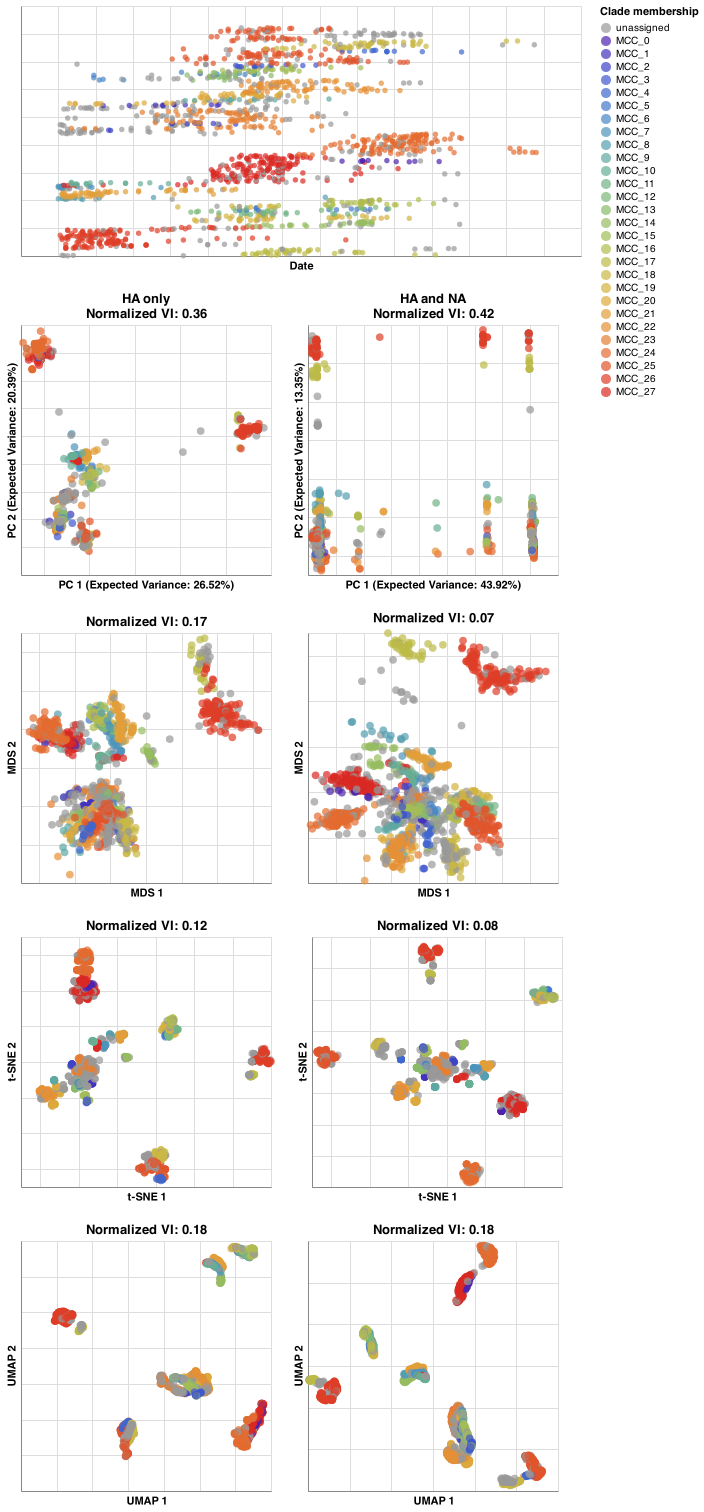
\includegraphics[width=\columnwidth]{figures/flu-2016-2018-ha-na-embeddings-by-mcc.png}
\caption{{\bf Embeddings of seasonal influenza HA-only (first column) and concatenated HA/NA sequences (second column) colored by TreeKnit Maximally Compatible Clades (MCCs) label.}
  The first normalized VI values per embedding reflect the distance between HA/NA clusters and known genetic groups (MCCs).
  VI values in parentheses reflect the distance between HA-only clusters and known genetic groups.
}
\label{fig:seasonal-influenza-h3n2-ha-na-2016-2018-embeddings}
\end{figure}

\begin{figure}[!h]
% TODO: remove includegraphics commands in final submission; figures must be uploaded separately from the manuscript.
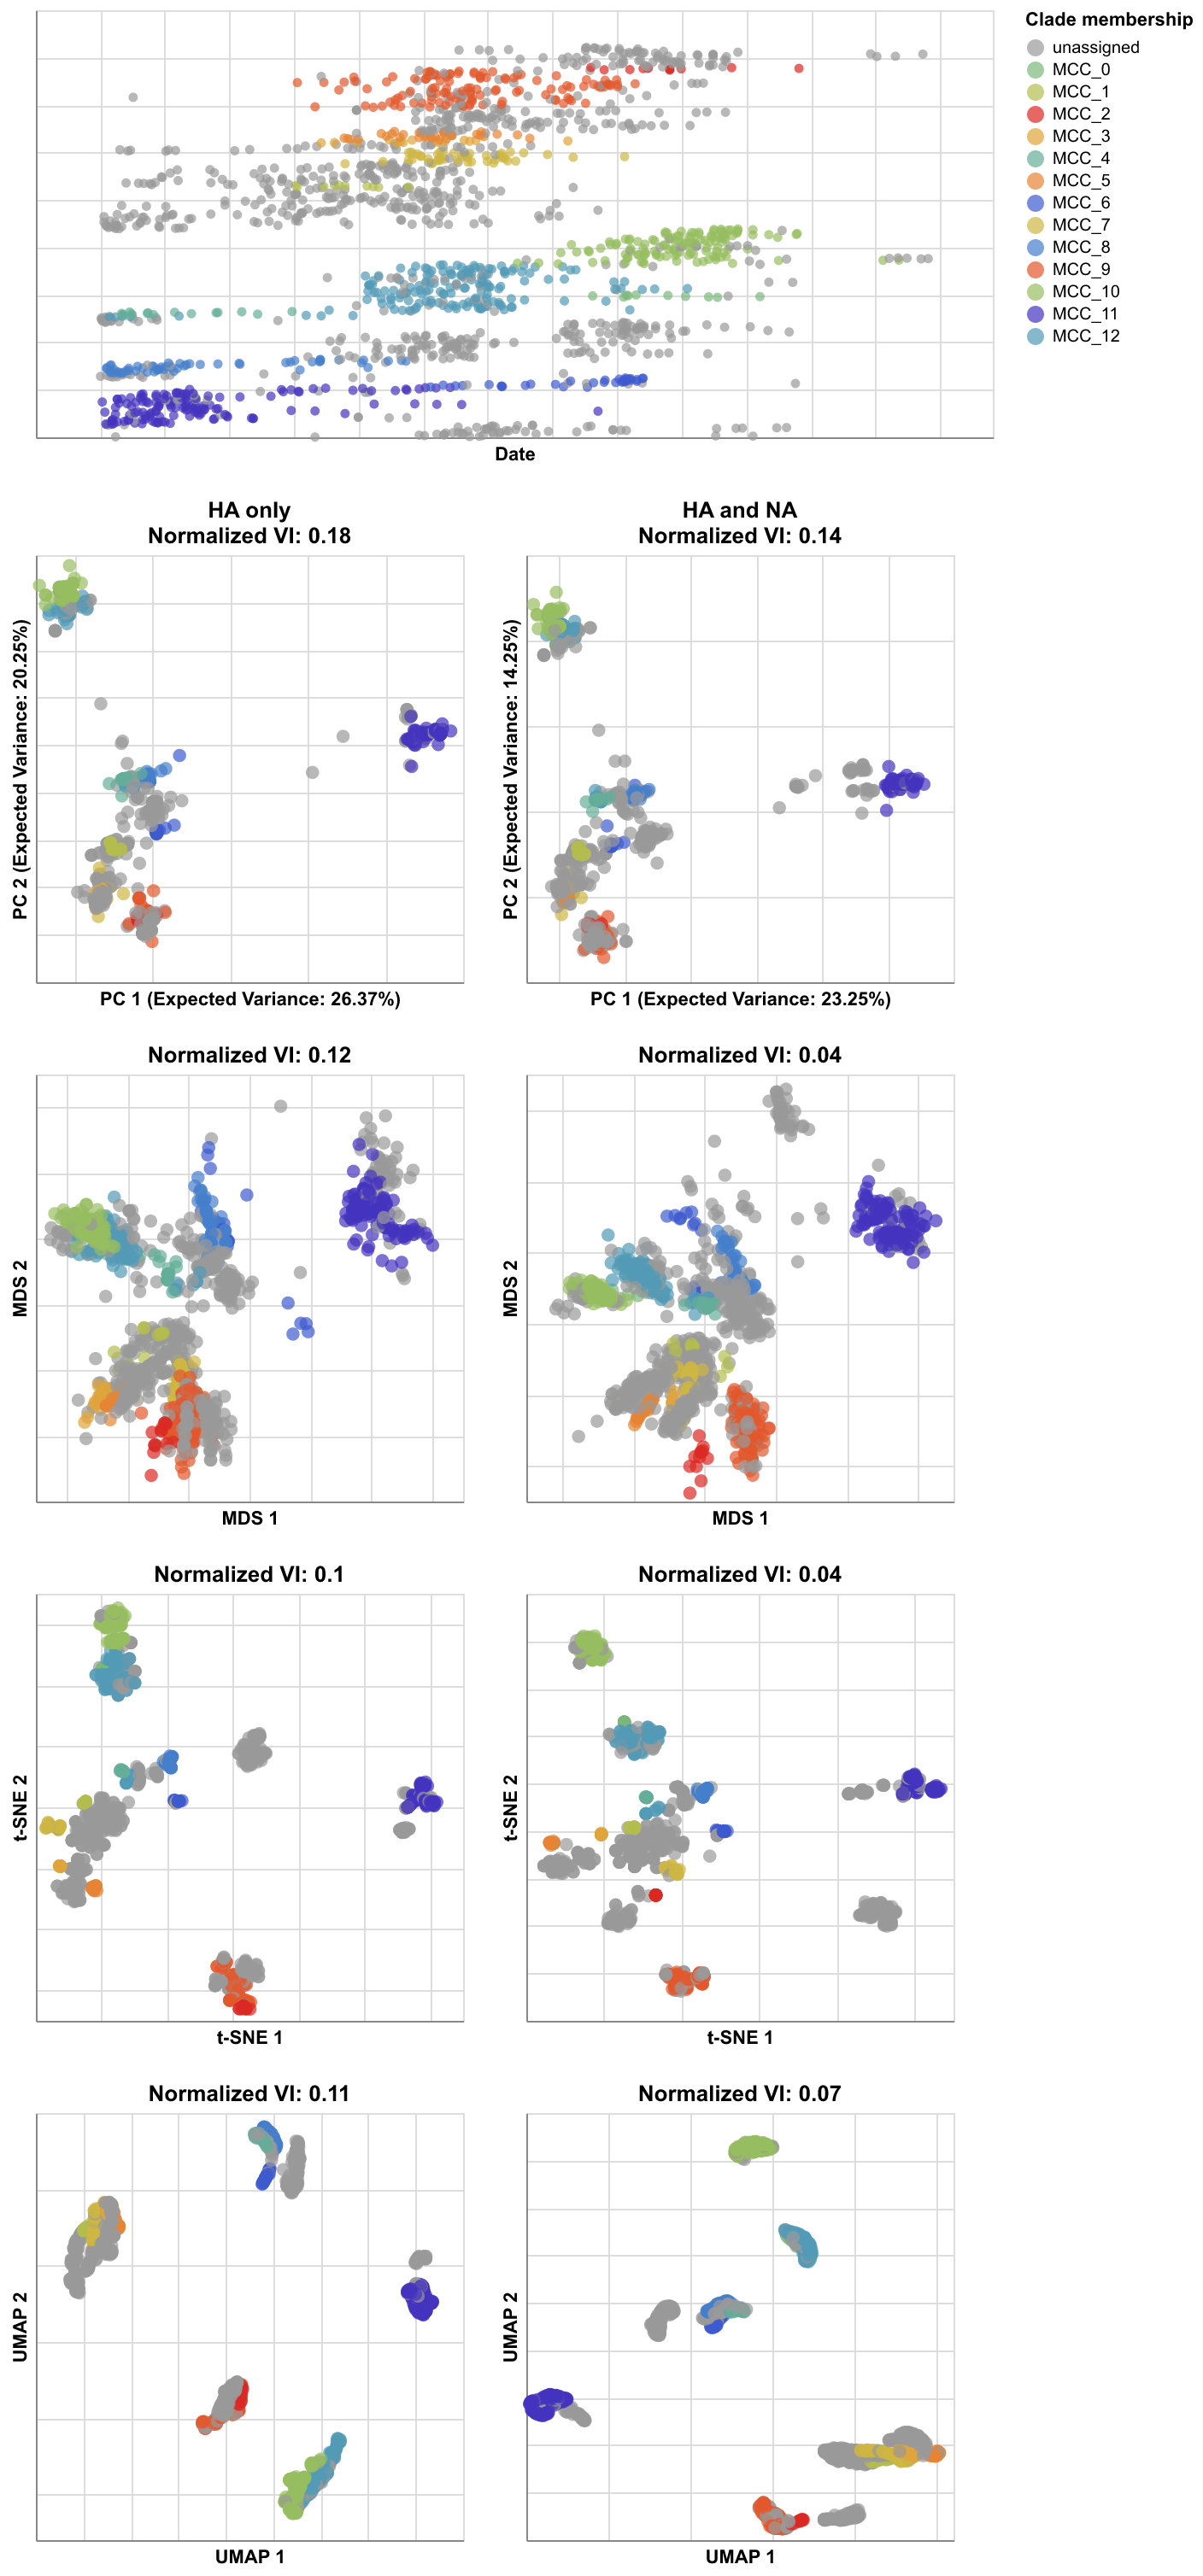
\includegraphics[width=0.75\columnwidth]{figures/flu-2016-2018-ha-na-all-embeddings-by-mcc.png}
\caption*{{\bf S8 Fig. Embeddings influenza H3N2 HA-only (left) and combined HA/NA (right) showing the effects of additional NA genetic information on the placement of reassortment events detected by TreeKnit (MCCs).}}
\end{figure}

\begin{figure}[!h]
% TODO: remove includegraphics commands in final submission; figures must be uploaded separately from the manuscript.
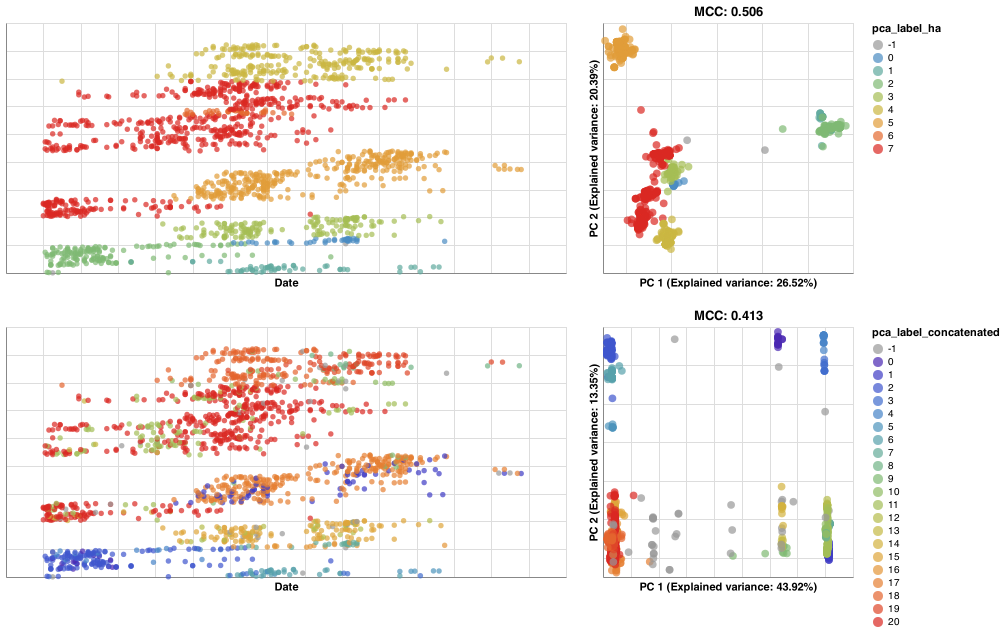
\includegraphics[width=\columnwidth]{figures/flu-2016-2018-ha-na-pca-by-cluster.png}
\caption*{{\bf S9 Fig. PCA embeddings for influenza H3N2 HA sequences only (top row) and HA/NA sequences combined (bottom row) showing the HA trees colored by clusters identified in each embedding (left) and the corresponding embeddings colored by cluster (right).}}
\end{figure}

\begin{figure}[!h]
% TODO: remove includegraphics commands in final submission; figures must be uploaded separately from the manuscript.
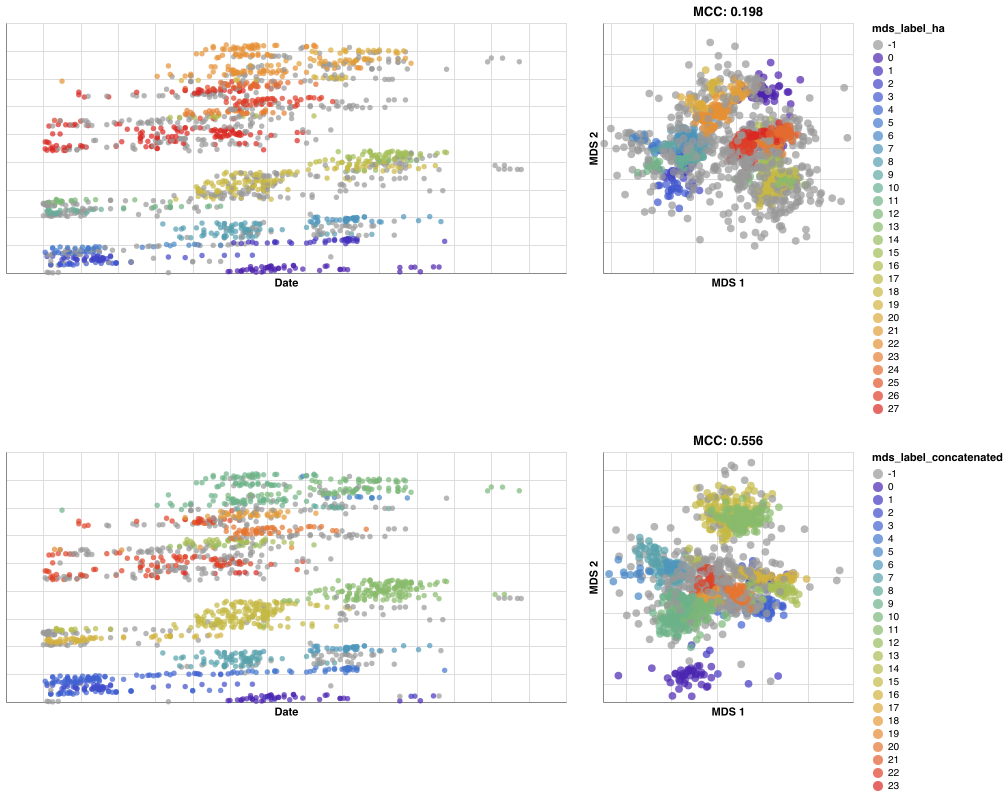
\includegraphics[width=\columnwidth]{figures/flu-2016-2018-ha-na-mds-by-cluster.png}
\caption*{{\bf S10 Fig. MDS embeddings for influenza H3N2 HA sequences only (top row) and HA/NA sequences combined (bottom row) showing the HA trees colored by clusters identified in each embedding (left) and the corresponding embeddings colored by cluster (right).}}
\end{figure}

\begin{figure}[!h]
% TODO: remove includegraphics commands in final submission; figures must be uploaded separately from the manuscript.
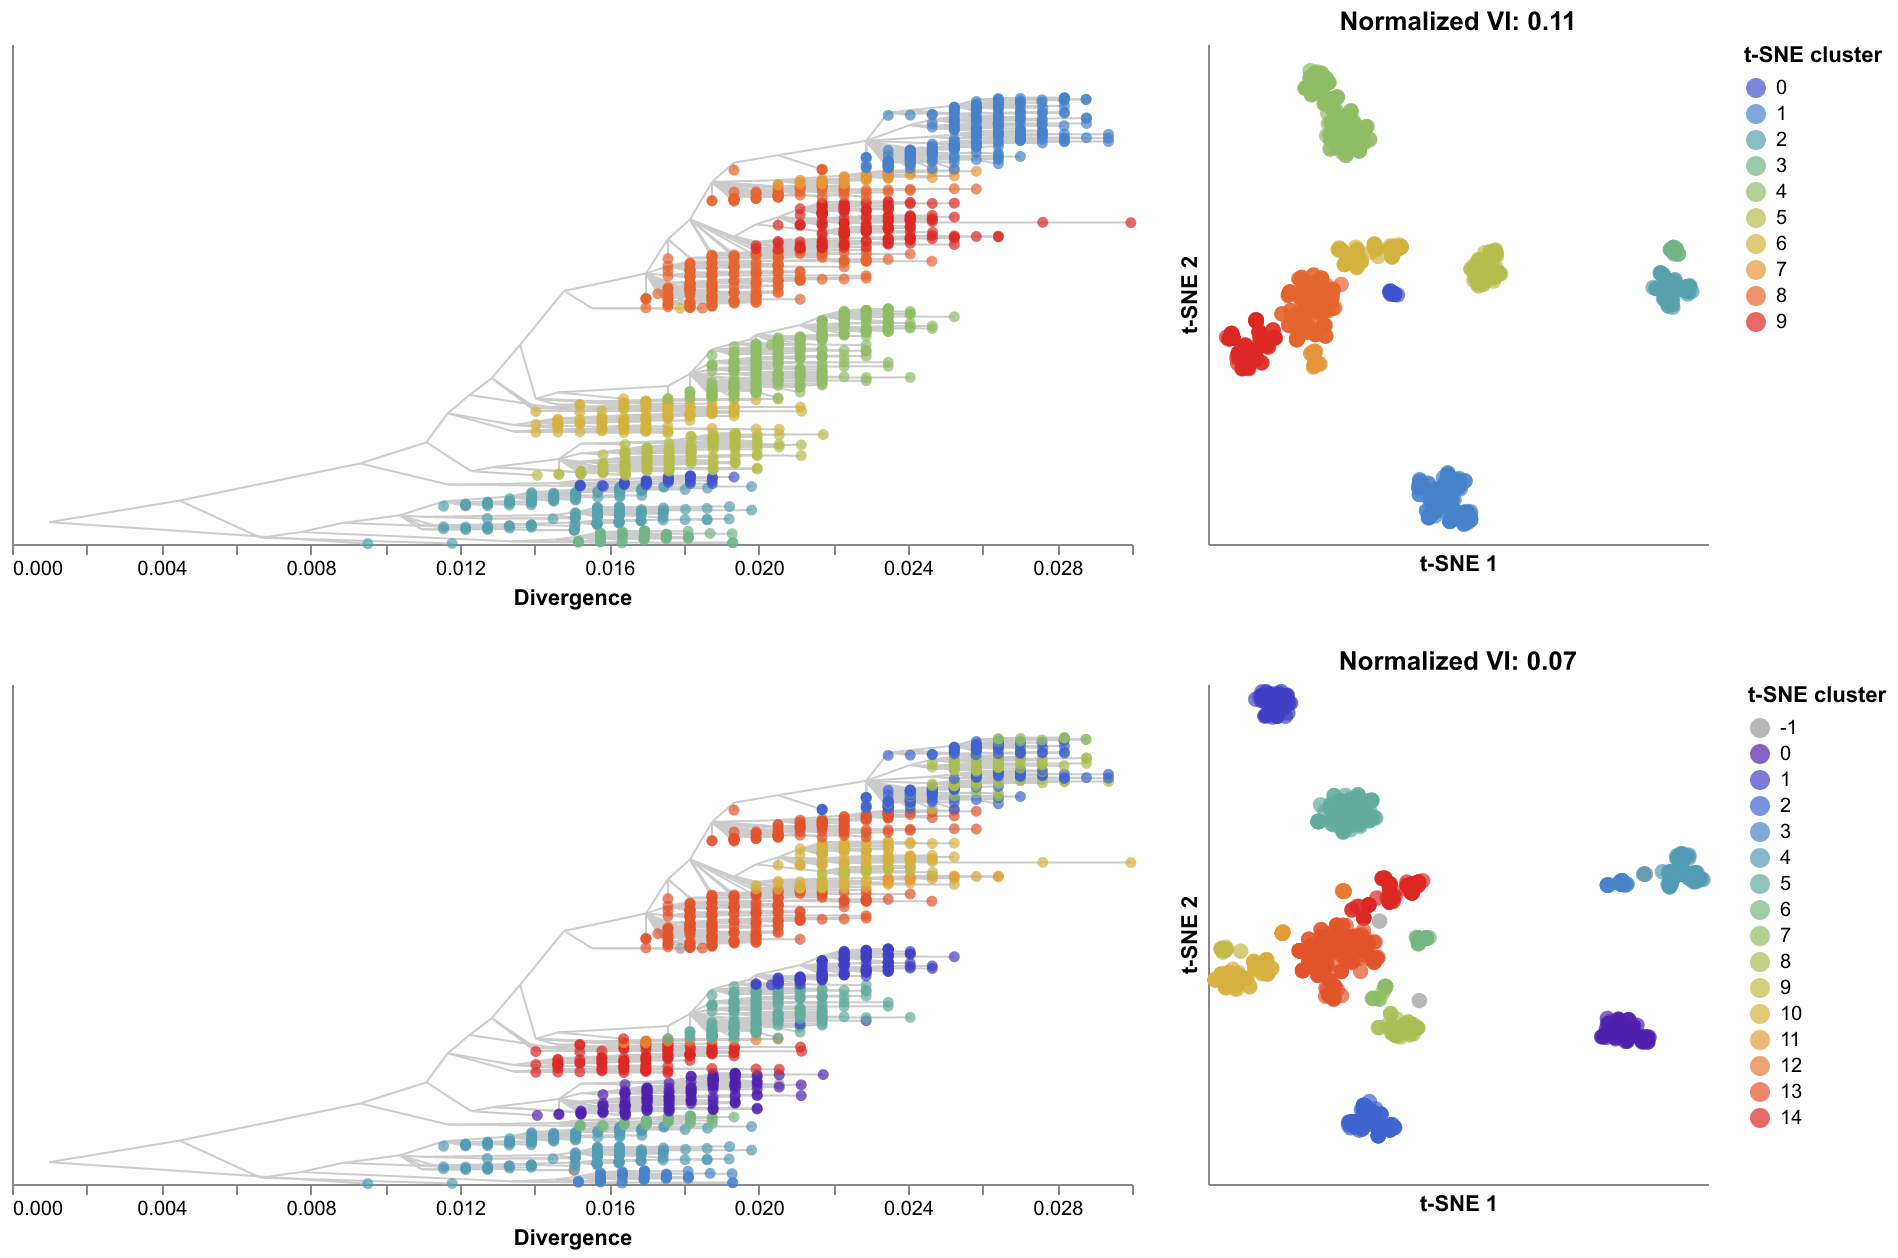
\includegraphics[width=\columnwidth]{figures/flu-2016-2018-ha-na-tsne-by-cluster.png}
\caption*{{\bf S11 Fig. t-SNE embeddings for influenza H3N2 HA sequences only (top row) and HA/NA sequences combined (bottom row) showing the HA trees colored by clusters identified in each embedding (left) and the corresponding embeddings colored by cluster (right).}}
\end{figure}

\begin{figure}[!h]
% TODO: remove includegraphics commands in final submission; figures must be uploaded separately from the manuscript.
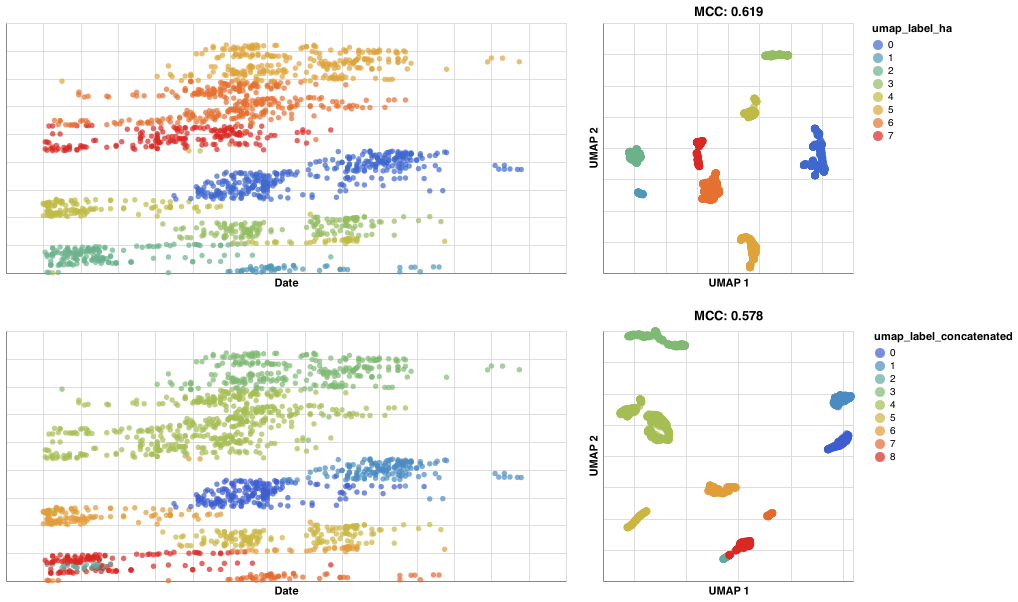
\includegraphics[width=\columnwidth]{figures/flu-2016-2018-ha-na-umap-by-cluster.png}
\caption*{{\bf S12 Fig. UMAP embeddings for influenza H3N2 HA sequences only (top row) and HA/NA sequences combined (bottom row) showing the HA trees colored by clusters identified in each embedding (left) and the corresponding embeddings colored by cluster (right).}}
\end{figure}

\subsection*{SARS-CoV-2 clusters recapitulate broad genetic groups corresponding to Nextstrain clades}

SARS-CoV-2 poses a greater challenge to embedding methods than seasonal influenza, with an unsegmented genome an order of magnitude longer than influenza's HA or NA \cite{Zhu2020}, a mutation rate in the spike surface protein subunit S1 that is four times higher than influenza H3N2's HA rate \cite{Kistler2022}, and increasingly common recombination \cite{Focosi2022,Turakhia2022}.
However, multiple expert- and model-based clade definitions exist for SARS-CoV-2, enabling comparison between clusters from embeddings and known genetic groups.
These definitions span from broad genetic groups named by the WHO as ``variants of concern'' (e.g., ``Alpha'', ``Beta'', etc.) \cite{Konings2021} or systematically defined by the Nextstrain team \cite{Hodcroft2020,Bedford2021,Roemer2022} to smaller, emerging genetic clusters defined by Pangolin \cite{OToole2021}.
As with seasonal influenza, we defined an ``early'' SARS-CoV-2 dataset spanning from January 2020 to January 2022, embedded genomes with the same four methods, and identified HDBSCAN clustering parameters that minimized the VI distance between embedding clusters and previously defined genetic groups as defined by Nextstrain clades and collapsed ``Nextclade pango'' lineages (see Methods).
Using these optimal cluster parameters, we produced clusters from embeddings of a ``late'' SARS-CoV-2 dataset spanning from January 2022 to November 2023 and calculated the VI distance between those clusters and known genetic groups.

The early SARS-CoV-2 dataset represented 23 Nextstrain clades and 35 collapsed Nextclade pango lineages.
With the exception of PCA, all other embedding methods placed samples from the same Nextstrain clades closer together and closely related Nextstrain clades near each other (Fig.~\ref{fig:sars-cov-2-early-embeddings-by-Nextstrain-clade}).
For example, the most genetically distinct clades like 21J (Delta) and 21K (Omicron) placed farthest from other clades, while all Delta clades (21A, 21I, and 21J) placed close together (Fig.~\ref{fig:sars-cov-2-early-embeddings-by-Nextstrain-clade}, \nameref{S13_Fig_sarscov2_early_mds}).
As we saw with embeddings of H3N2 HA sequences, MDS placed related clades closer together on a continuous scale, while t-SNE and UMAP produced more clearly separate groups of samples.
Unlike the H3N2 HA analysis, the PCA embedding of SARS-CoV-2 sequences failed to create any genetically meaningful clusters.
We suspected that PCA components reflected variation in missing (``N'') or gap (``-'') characters that we represented with a separate character state than the standard nucleotide characters of A, C, G, and T.
We plotted the PC1 value of each sample against the number of missing bases in its alignment and confirmed that missing data explained a substantial proportion of variation in PC1 (\nameref{S14_Fig_sarscov2_early_pc1_vs_bases_missing}, Pearson's $R^{2}=0.354$).
When we compared embedding clusters to Nextclade pango lineages, we did not observe the same clear grouping as we did with Nextstrain clades.
For example, the Nextstrain clade 21J (Delta) contained 11 pango lineages that all appeared to map into the same overlapping space in MDS, t-SNE, and UMAP embeddings (\nameref{S15_Fig_sarscov2_early_embeddings_by_Nextclade_pango}).
These results suggest that distance-based embedding methods can recapitulate broader genetic groups of SARS-CoV-2, but that these methods lack the resolution of finer groups defined by Pangolin.

\begin{figure}[!h]
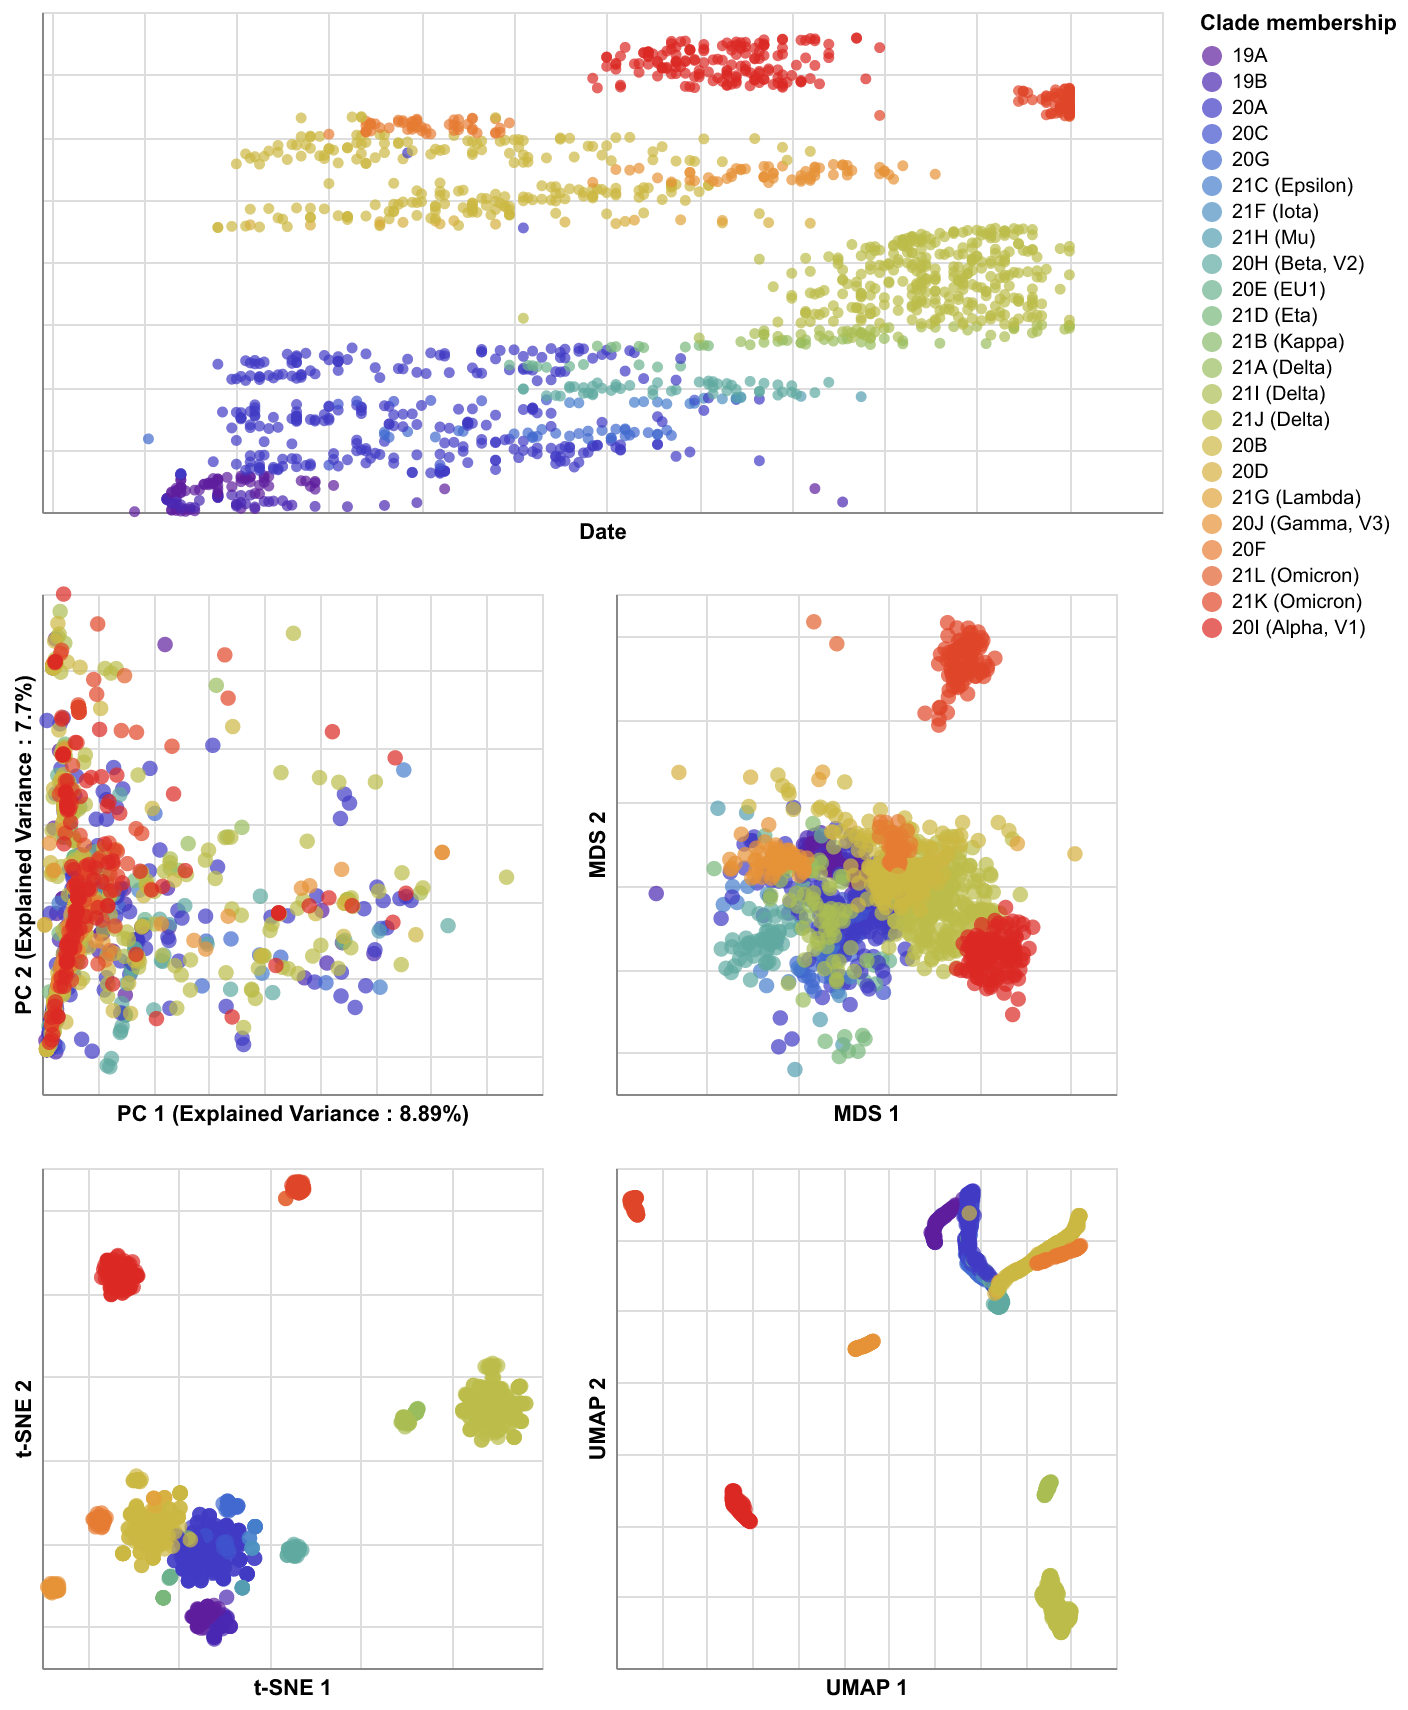
\includegraphics[width=\columnwidth]{figures/sarscov2-embeddings-by-Nextstrain_clade-clade.png}
\caption{{\bf Phylogeny and embeddings of SARS-CoV-2 sequences collected between January 1, 2020 and January 1, 2022 colored by Nextstrain clade label.}
}
\label{fig:sars-cov-2-early-embeddings-by-Nextstrain-clade}
\end{figure}

\begin{figure}[!h]
% TODO: remove includegraphics commands in final submission; figures must be uploaded separately from the manuscript.
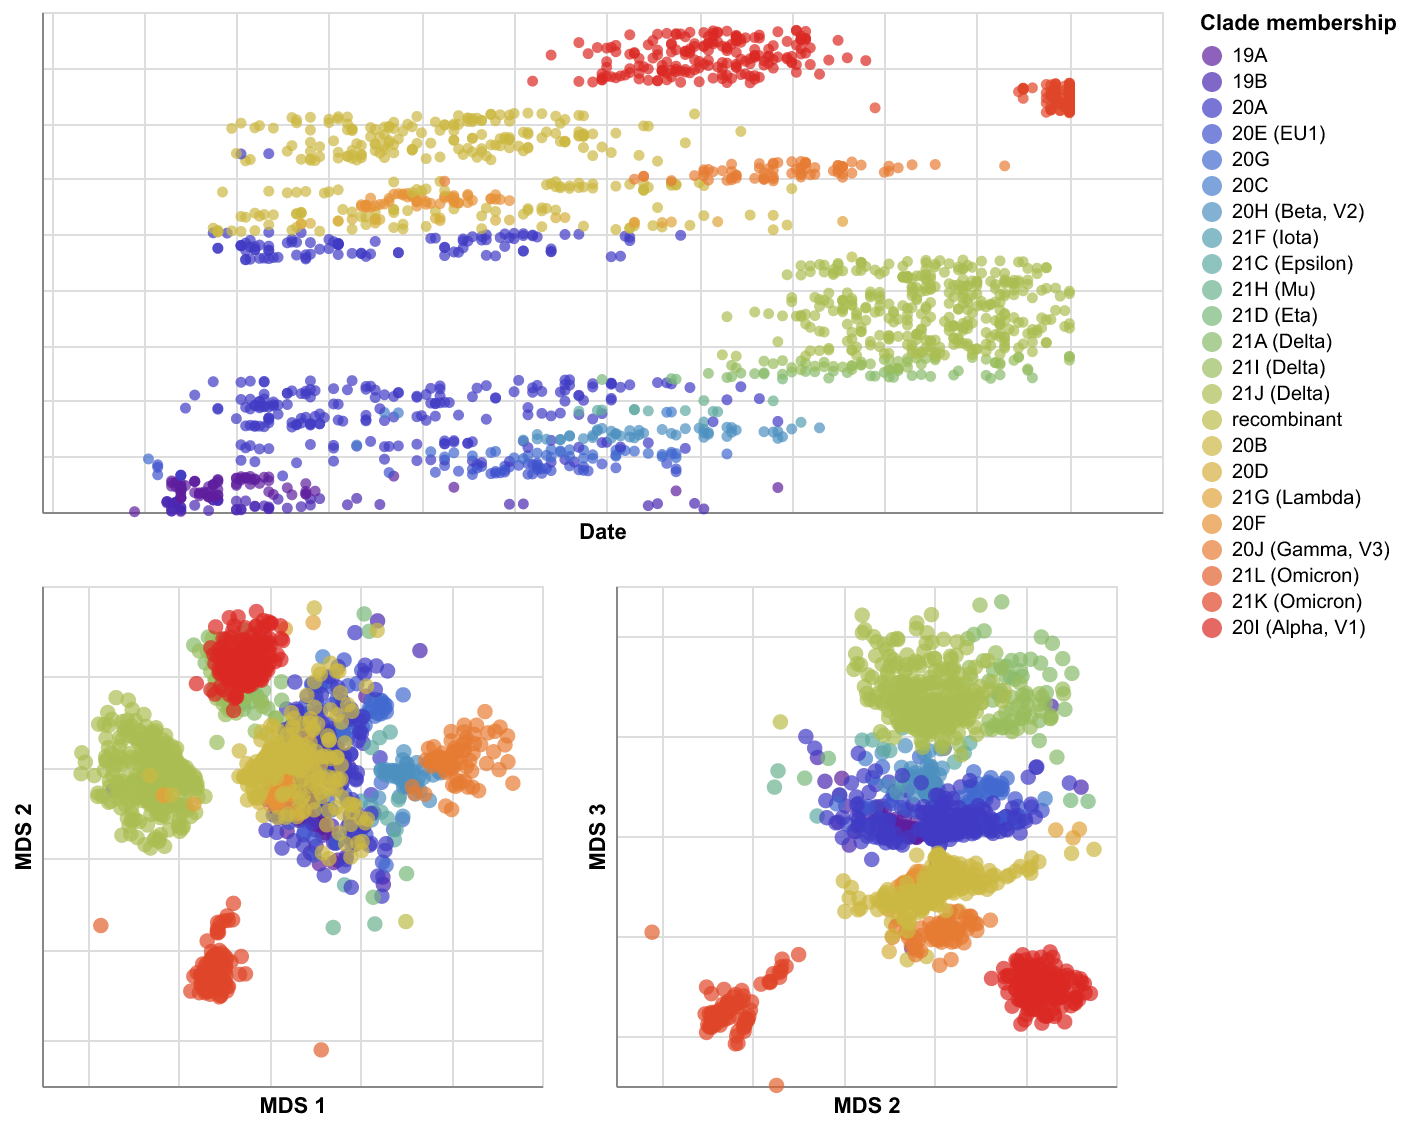
\includegraphics[width=\columnwidth]{figures/sarscov2-mds-by-Nextstrain_clade-clade.png}
\caption*{{\bf S13 Fig. MDS embeddings for early SARS-CoV-2 sequences showing all three components.}}
\end{figure}

\begin{figure}[!h]
% TODO: remove includegraphics commands in final submission; figures must be uploaded separately from the manuscript.
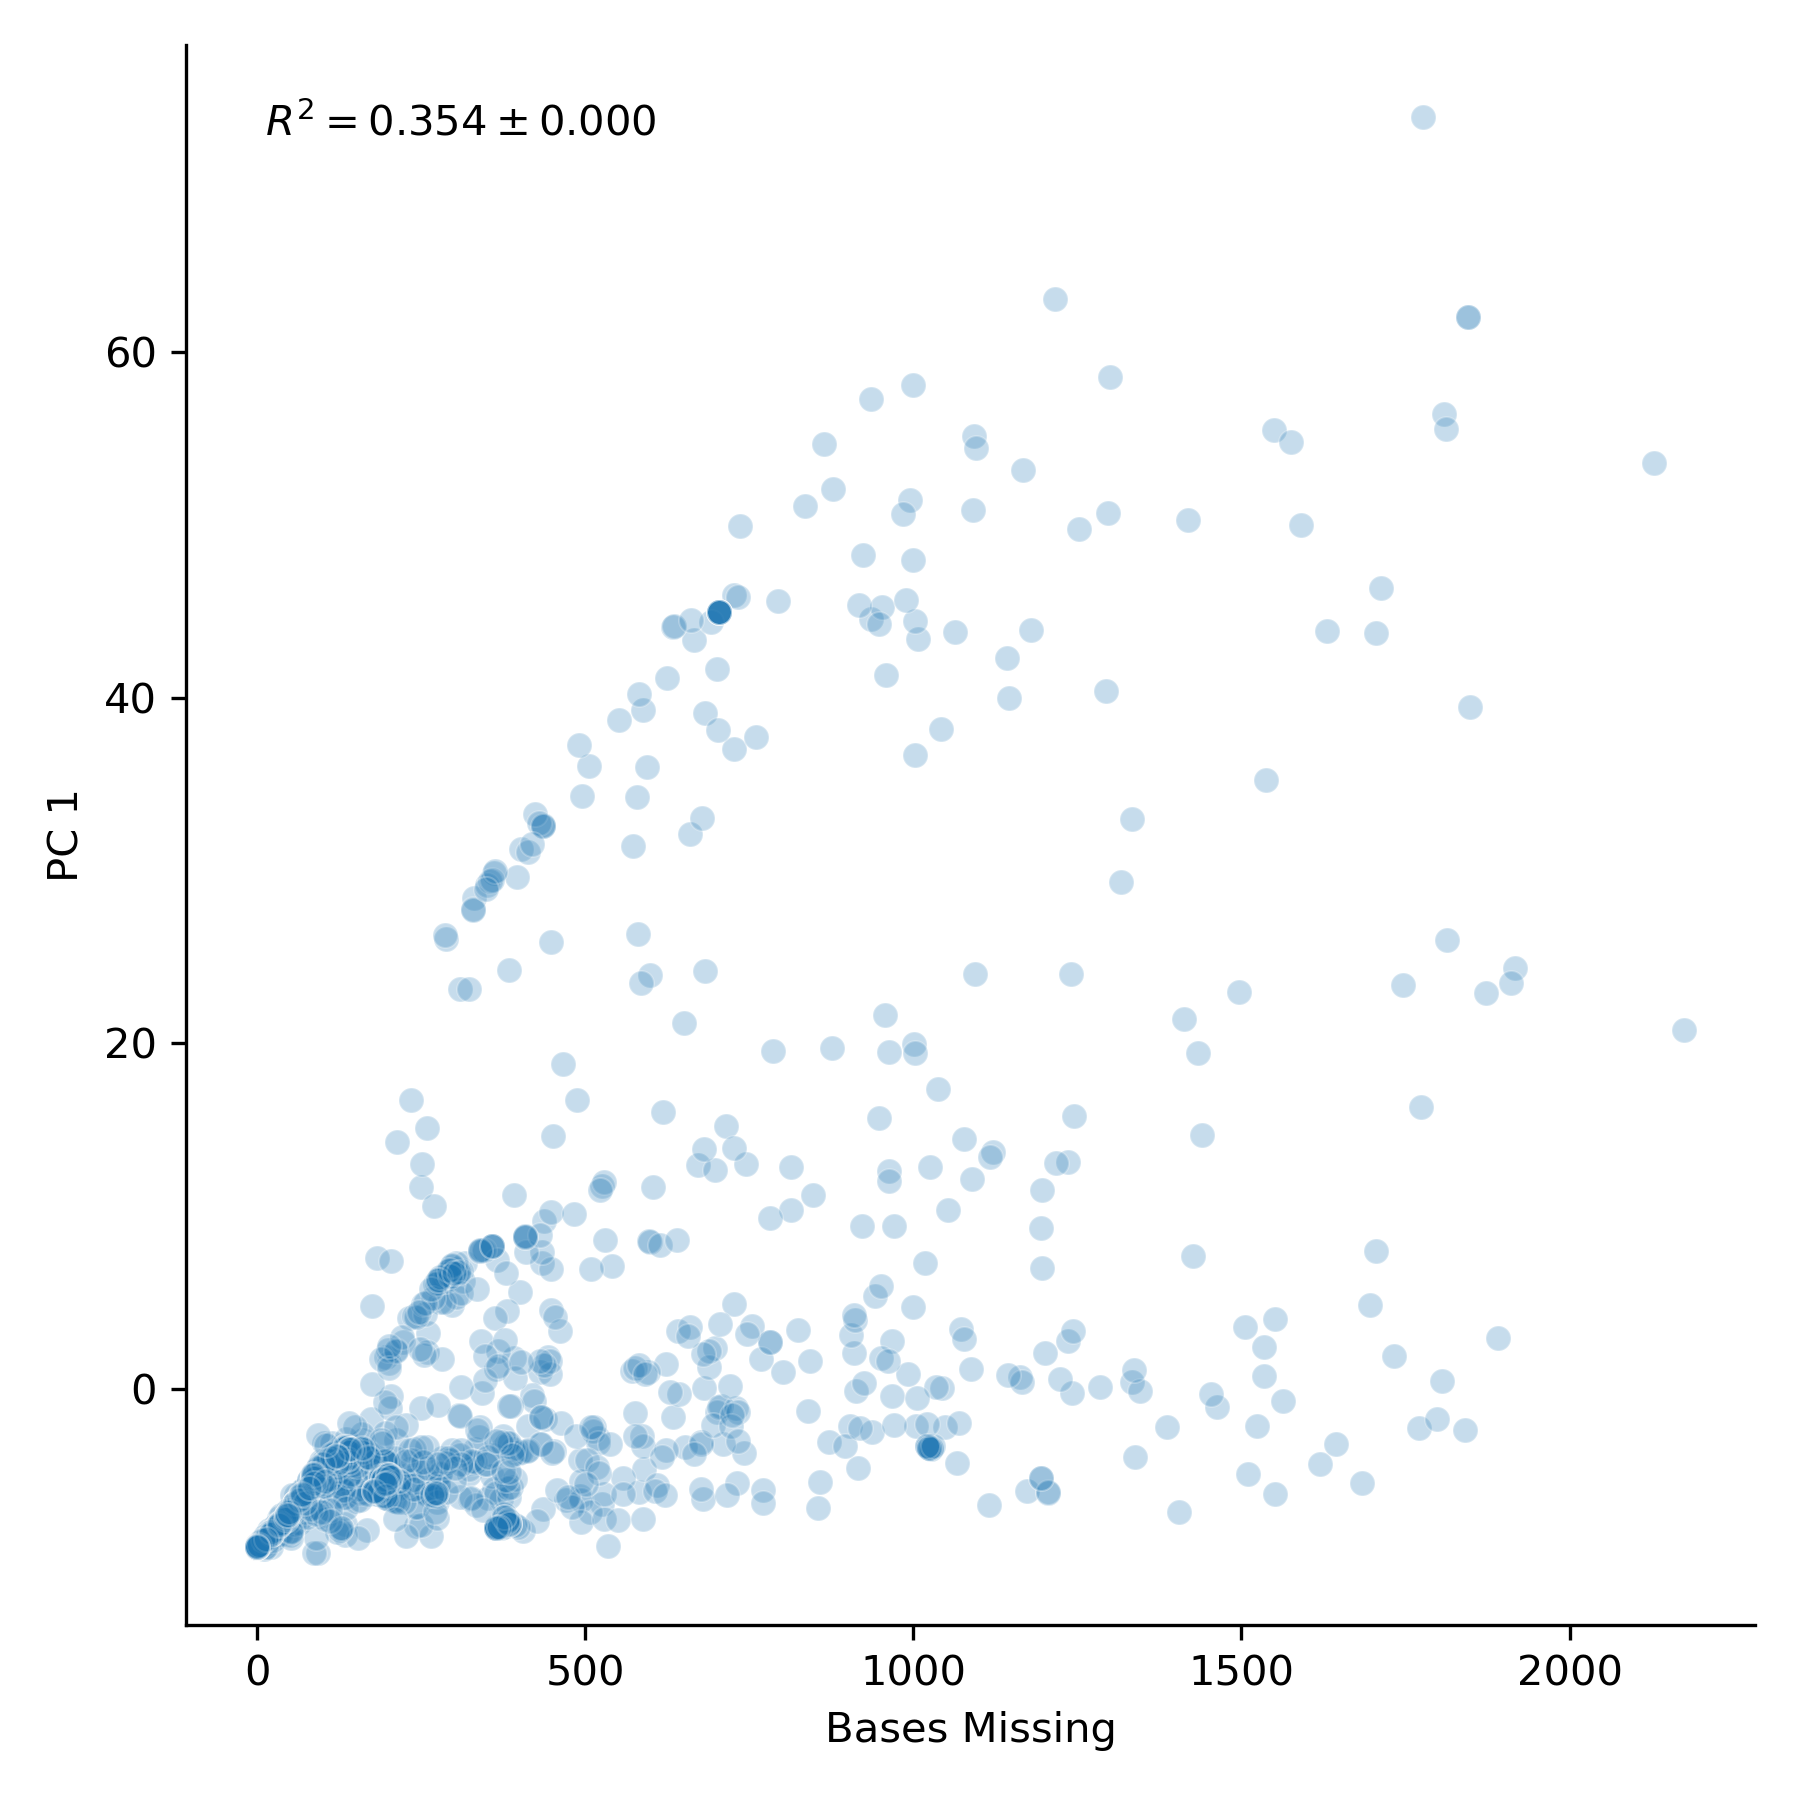
\includegraphics[width=\columnwidth]{figures/sarscov2-pc1-vs-bases-missing.png}
\caption*{{\bf S14 Fig. Principal component 1 (PC1) of the PCA embedding for early SARS-CoV-2 data plotted by the number of missing (``N'') or gap (``-'') characters in the corresponding sample's aligned sequence. Pearson's $R^{2}$ estimates the variation in PC1 explained by missing data.}}
\end{figure}

\begin{figure}[!h]
% TODO: remove includegraphics commands in final submission; figures must be uploaded separately from the manuscript.
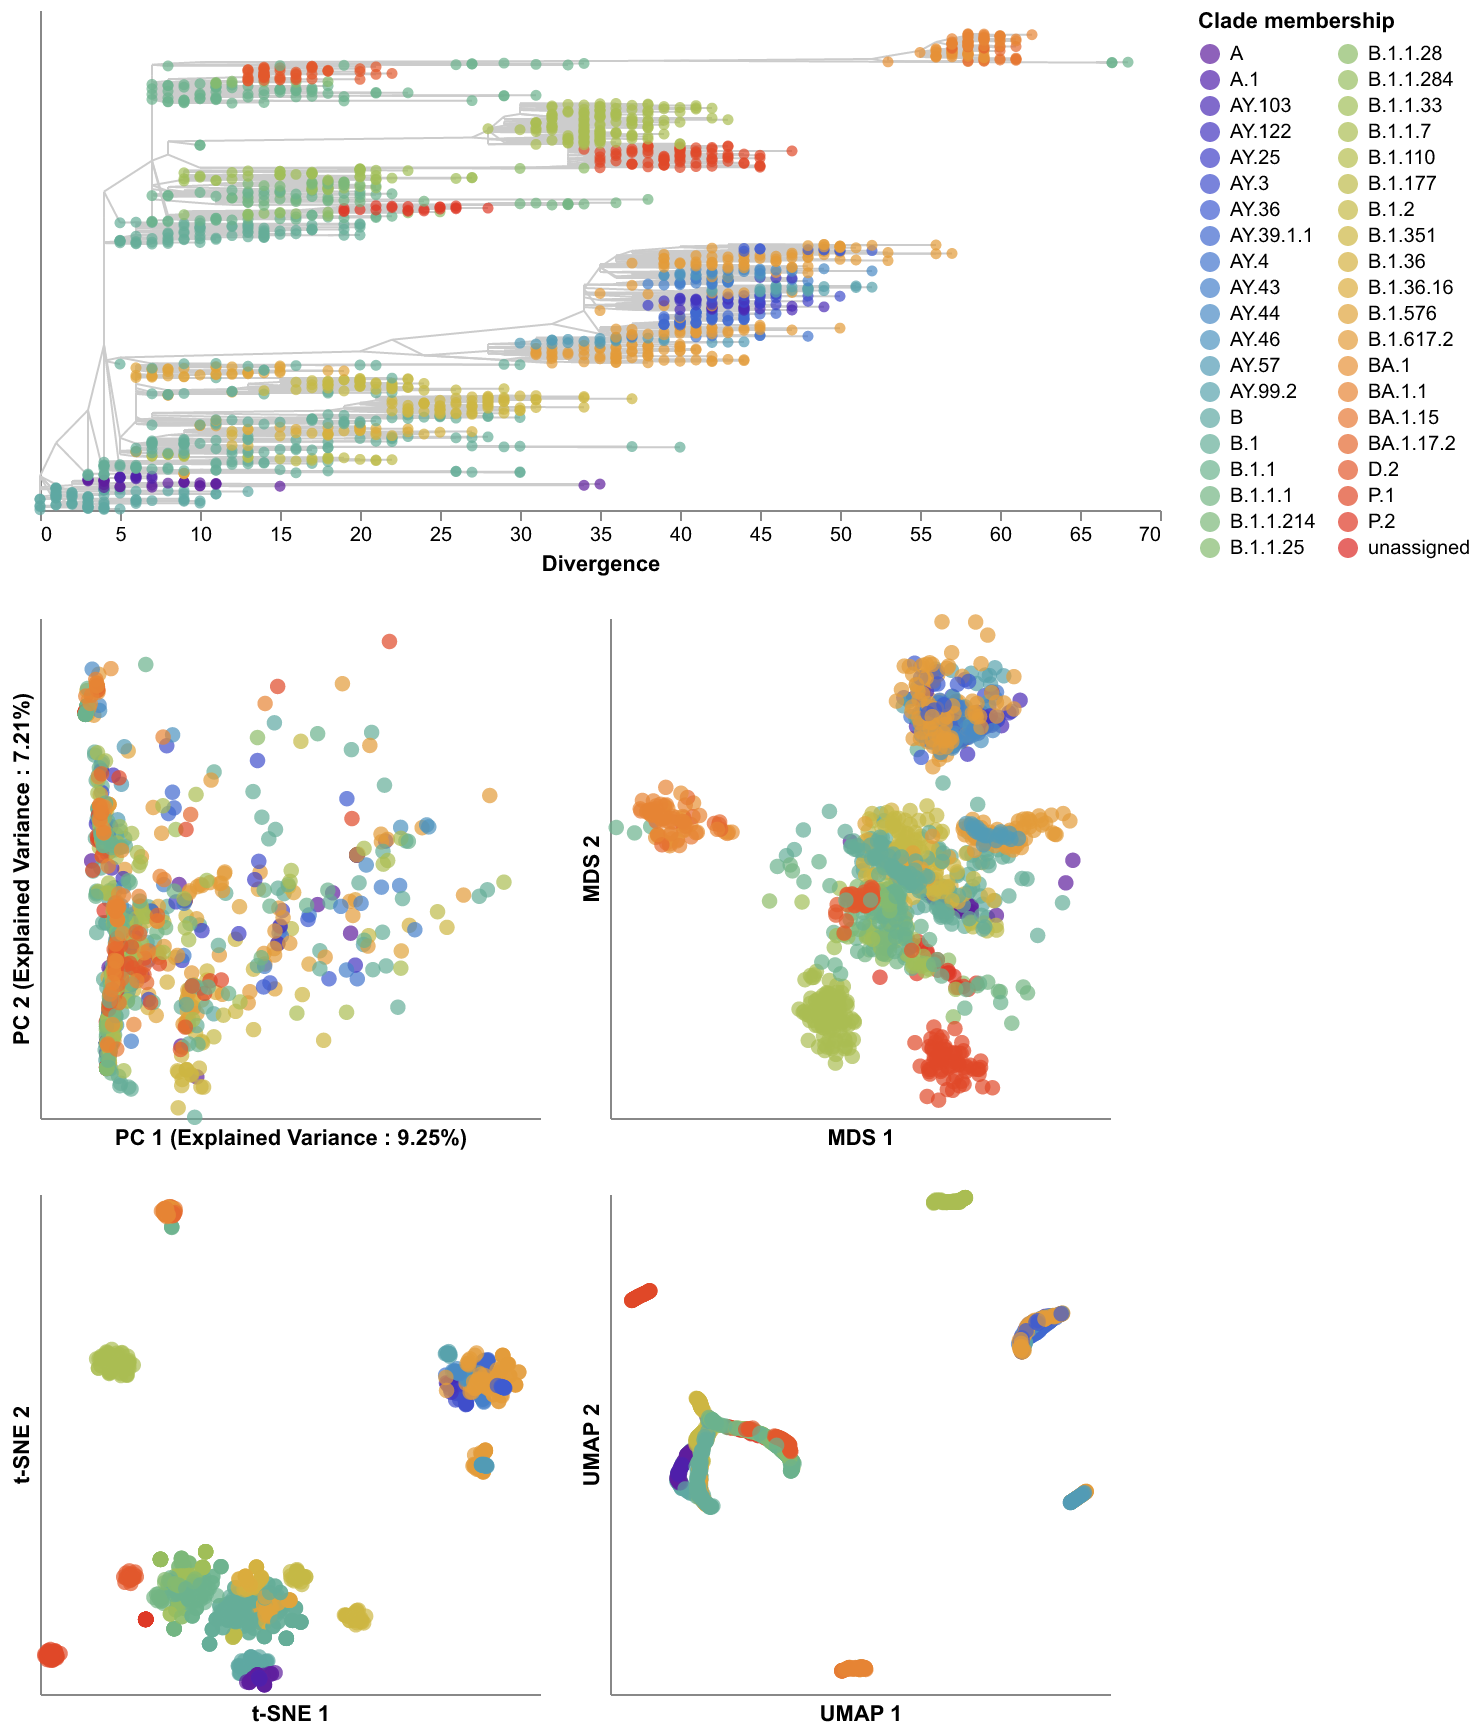
\includegraphics[width=\columnwidth]{figures/sarscov2-embeddings-by-Nextclade_pango_collapsed-clade.png}
\caption*{{\bf S15 Fig. Phylogeny and embeddings of SARS-CoV-2 sequences collected between January 1, 2020 and January 1, 2022 colored by collapsed Nextclade pango lineage label.}}
\end{figure}

We quantified the maintenance of local and global structure in early SARS-CoV-2 embeddings by fitting a linear model between pairwise genetic and Euclidean distances of samples.
As we expected from the qualitative evaluation of the PCA embedding above, we found no relationship between Euclidean distance in PCA and genetic distance in alignments (Fig.~\ref{fig:sars-cov-2-pairwise-distances}).
In contrast, the MDS embedding produced a strong linear mapping across the range of observed genetic distances (Pearson's $R^{2}=0.917$).
Both t-SNE and UMAP maintained intermediate degrees of linearity (Pearson's $R^{2}=0.617$ and $R^{2}=0.586$, respectively).
These embeddings placed the most genetically similar samples close together and the most genetically distinct farther apart.
However, these embeddings did not consistently place pairs of samples with intermediate genetic distances at an intermediate distance in Euclidean space.
The linear relationship for genetically similar samples in t-SNE remained consistent up to a genetic distance of approximately 30 nucleotides.
The corresponding relationship for UMAP only remained consistent up to a genetic distance of approximately 15 nucleotides.

\begin{figure}[!h]
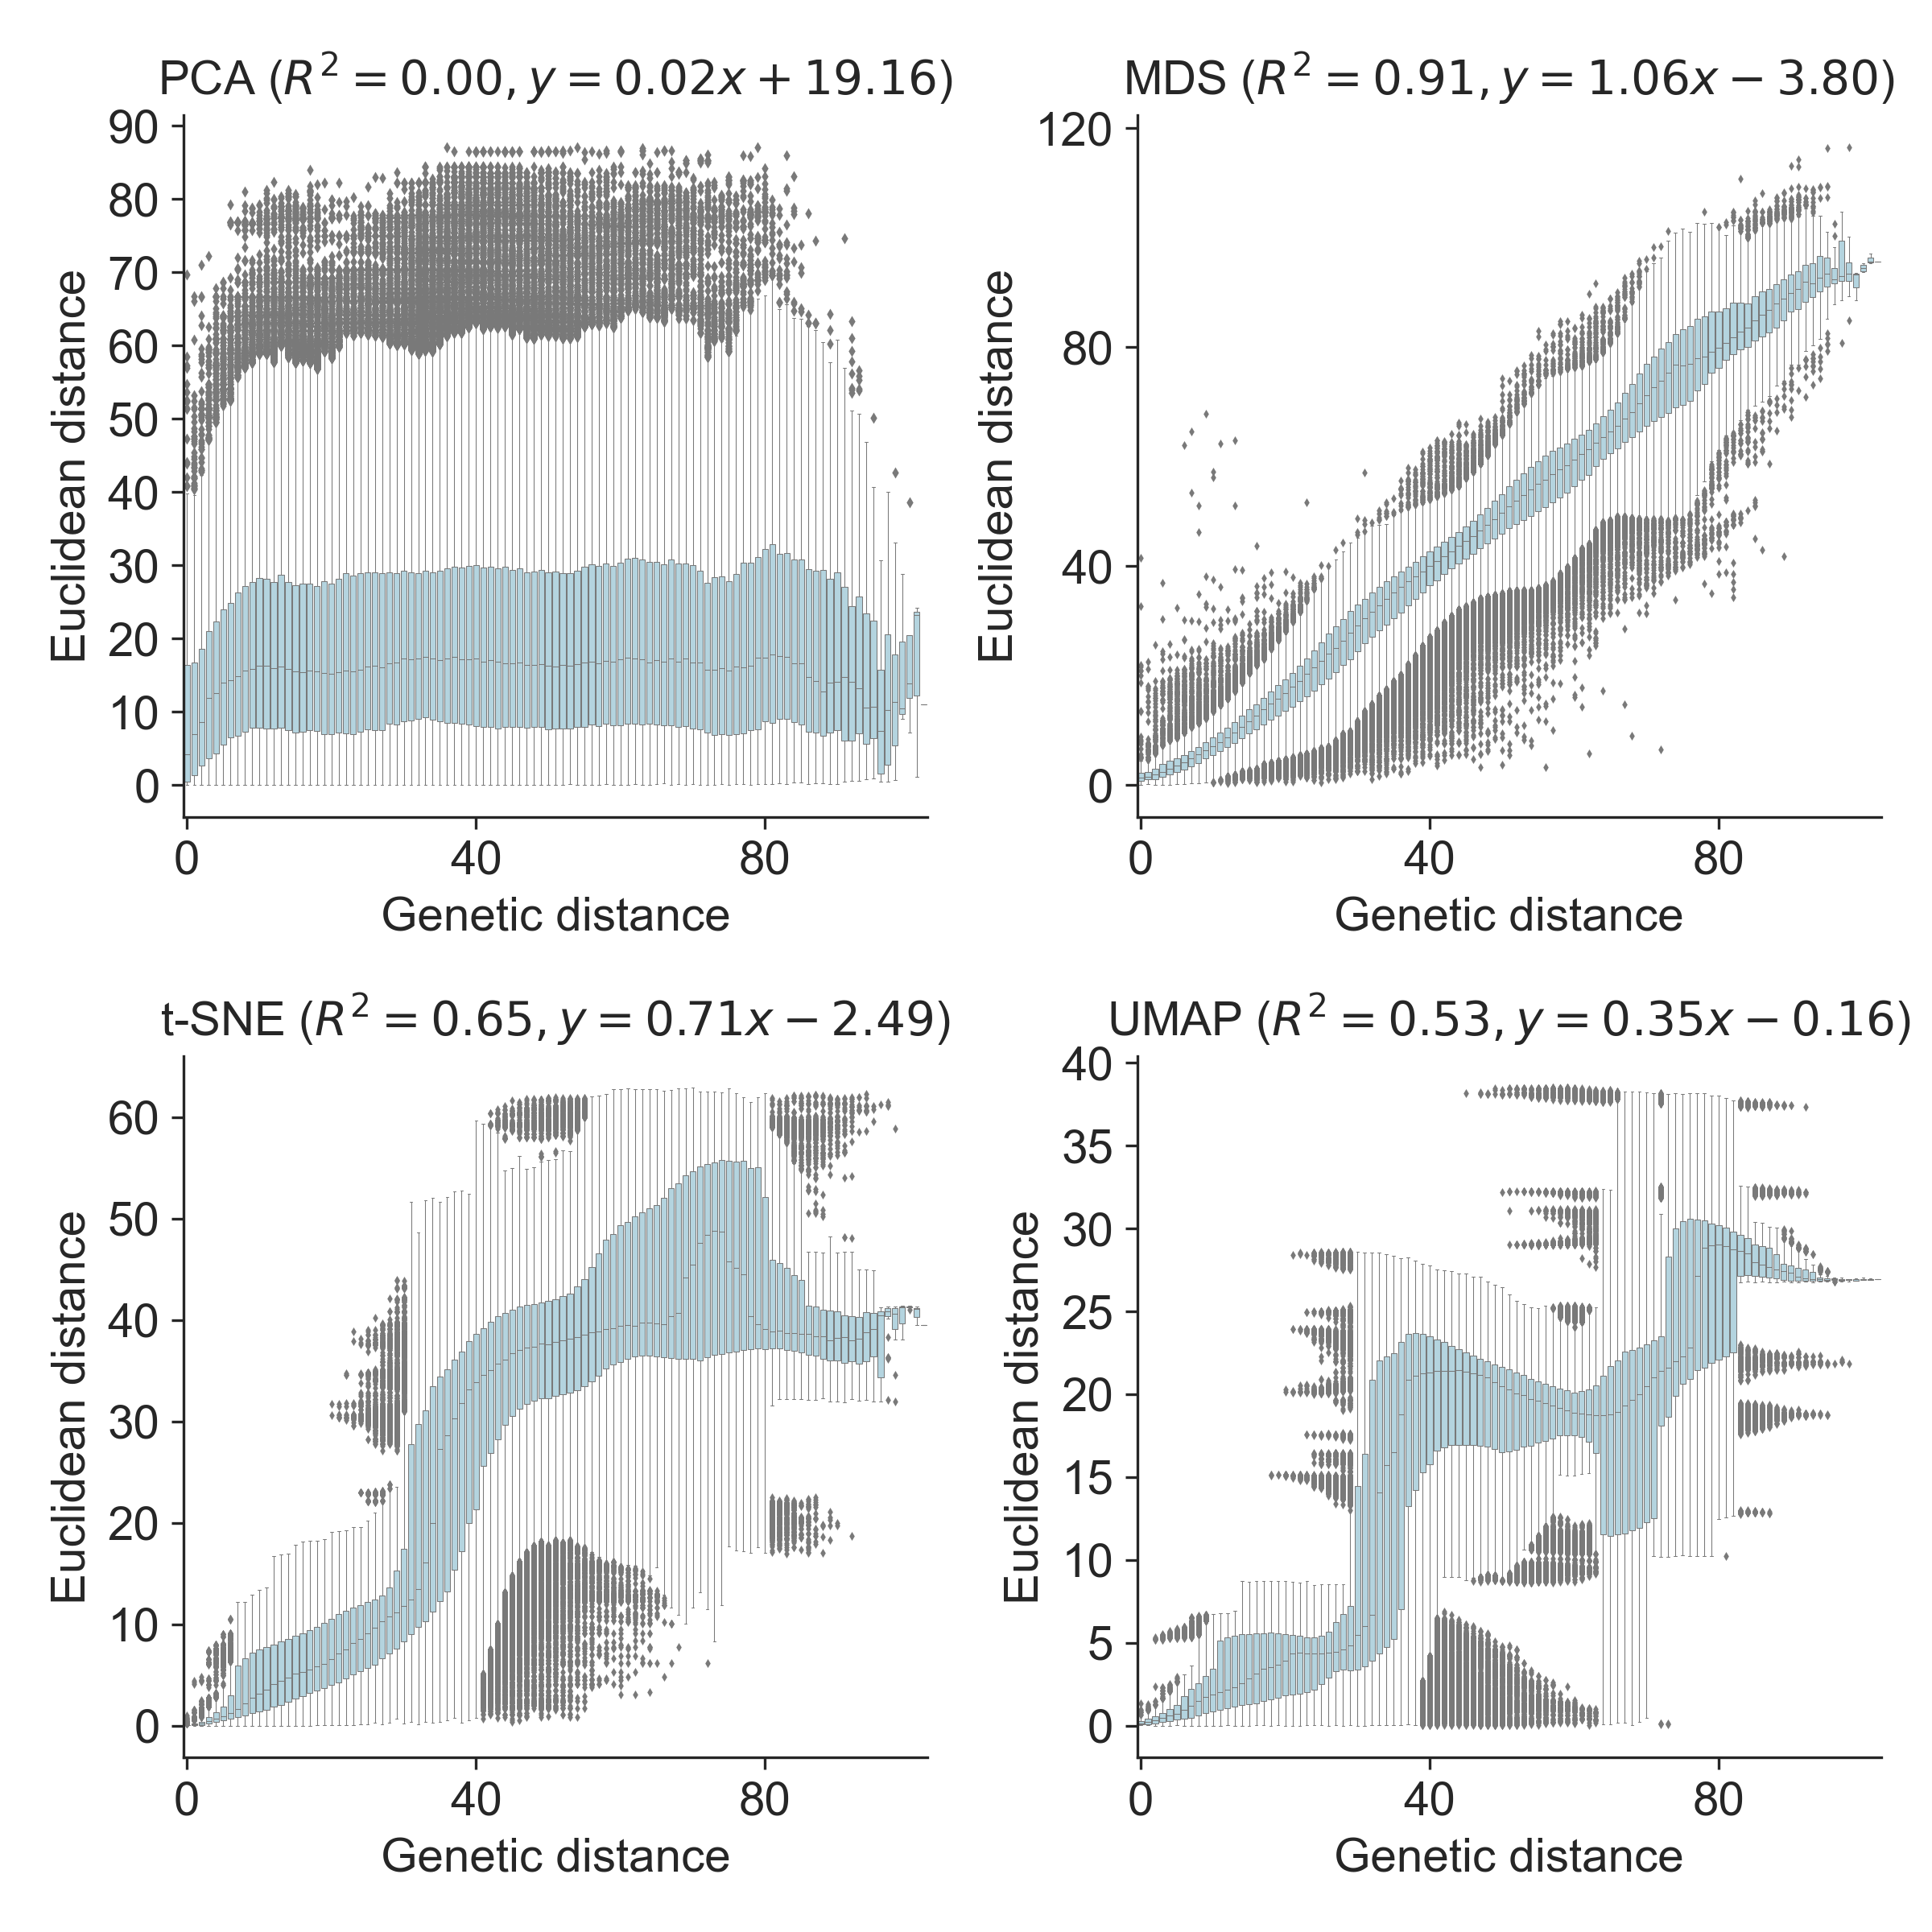
\includegraphics[width=\columnwidth]{figures/sarscov2-euclidean-distance-by-genetic-distance.png}
\caption{{\bf Relationship between pairwise genetic and Euclidean distances in embeddings for early (2020--2022) SARS-CoV-2 samples with PCA (upper left), MDS (upper right), t-SNE (lower left), and UMAP (lower right).}}
\label{fig:sars-cov-2-pairwise-distances}
\end{figure}

We identified clusters in embeddings from early SARS-CoV-2 data using cluster parameters that minimized the normalized VI distance between clusters and known genetic groups.
Since Nextstrain clades and Nextclade pango lineages represented different resolutions of genetic diversity, we identified separate optimal parameters for clusters compared to each of these known genetic groups.
When comparing clusters to Nextstrain clades, the t-SNE embedding produced the most accurate clusters with a normalized VI of 0.09 (N=14 clusters, minimum distance of 1.5) (Fig.~\ref{fig:sars-cov-2-2020-2022-clusters-vs-Nextstrain-clade}, Table~\ref{table:accuracy}).
MDS and UMAP produced similarly accurate clusters with normalized VIs of 0.14 (N=11) and 0.15 (N=6) at minimum distances of 0 and 0.5, respectively.
As expected, PCA produced the least accurate clusters with a normalized VI of 0.37 (N=2, minimum distance of 4.0).
We found 21 cluster-specific mutations for one of the two PCA clusters (all deletions), 161 for seven of 11 MDS clusters, 175 for 11 of 14 t-SNE clusters, and 149 for five of six UMAP clusters (\nameref{S1_Table}).
Clusters from t-SNE produced within-group genetic distances that were most similar to distances within Nextstrain clades (\nameref{S16_Fig_sarscov2_within_between_group_distances}).

\begin{figure}[!h]
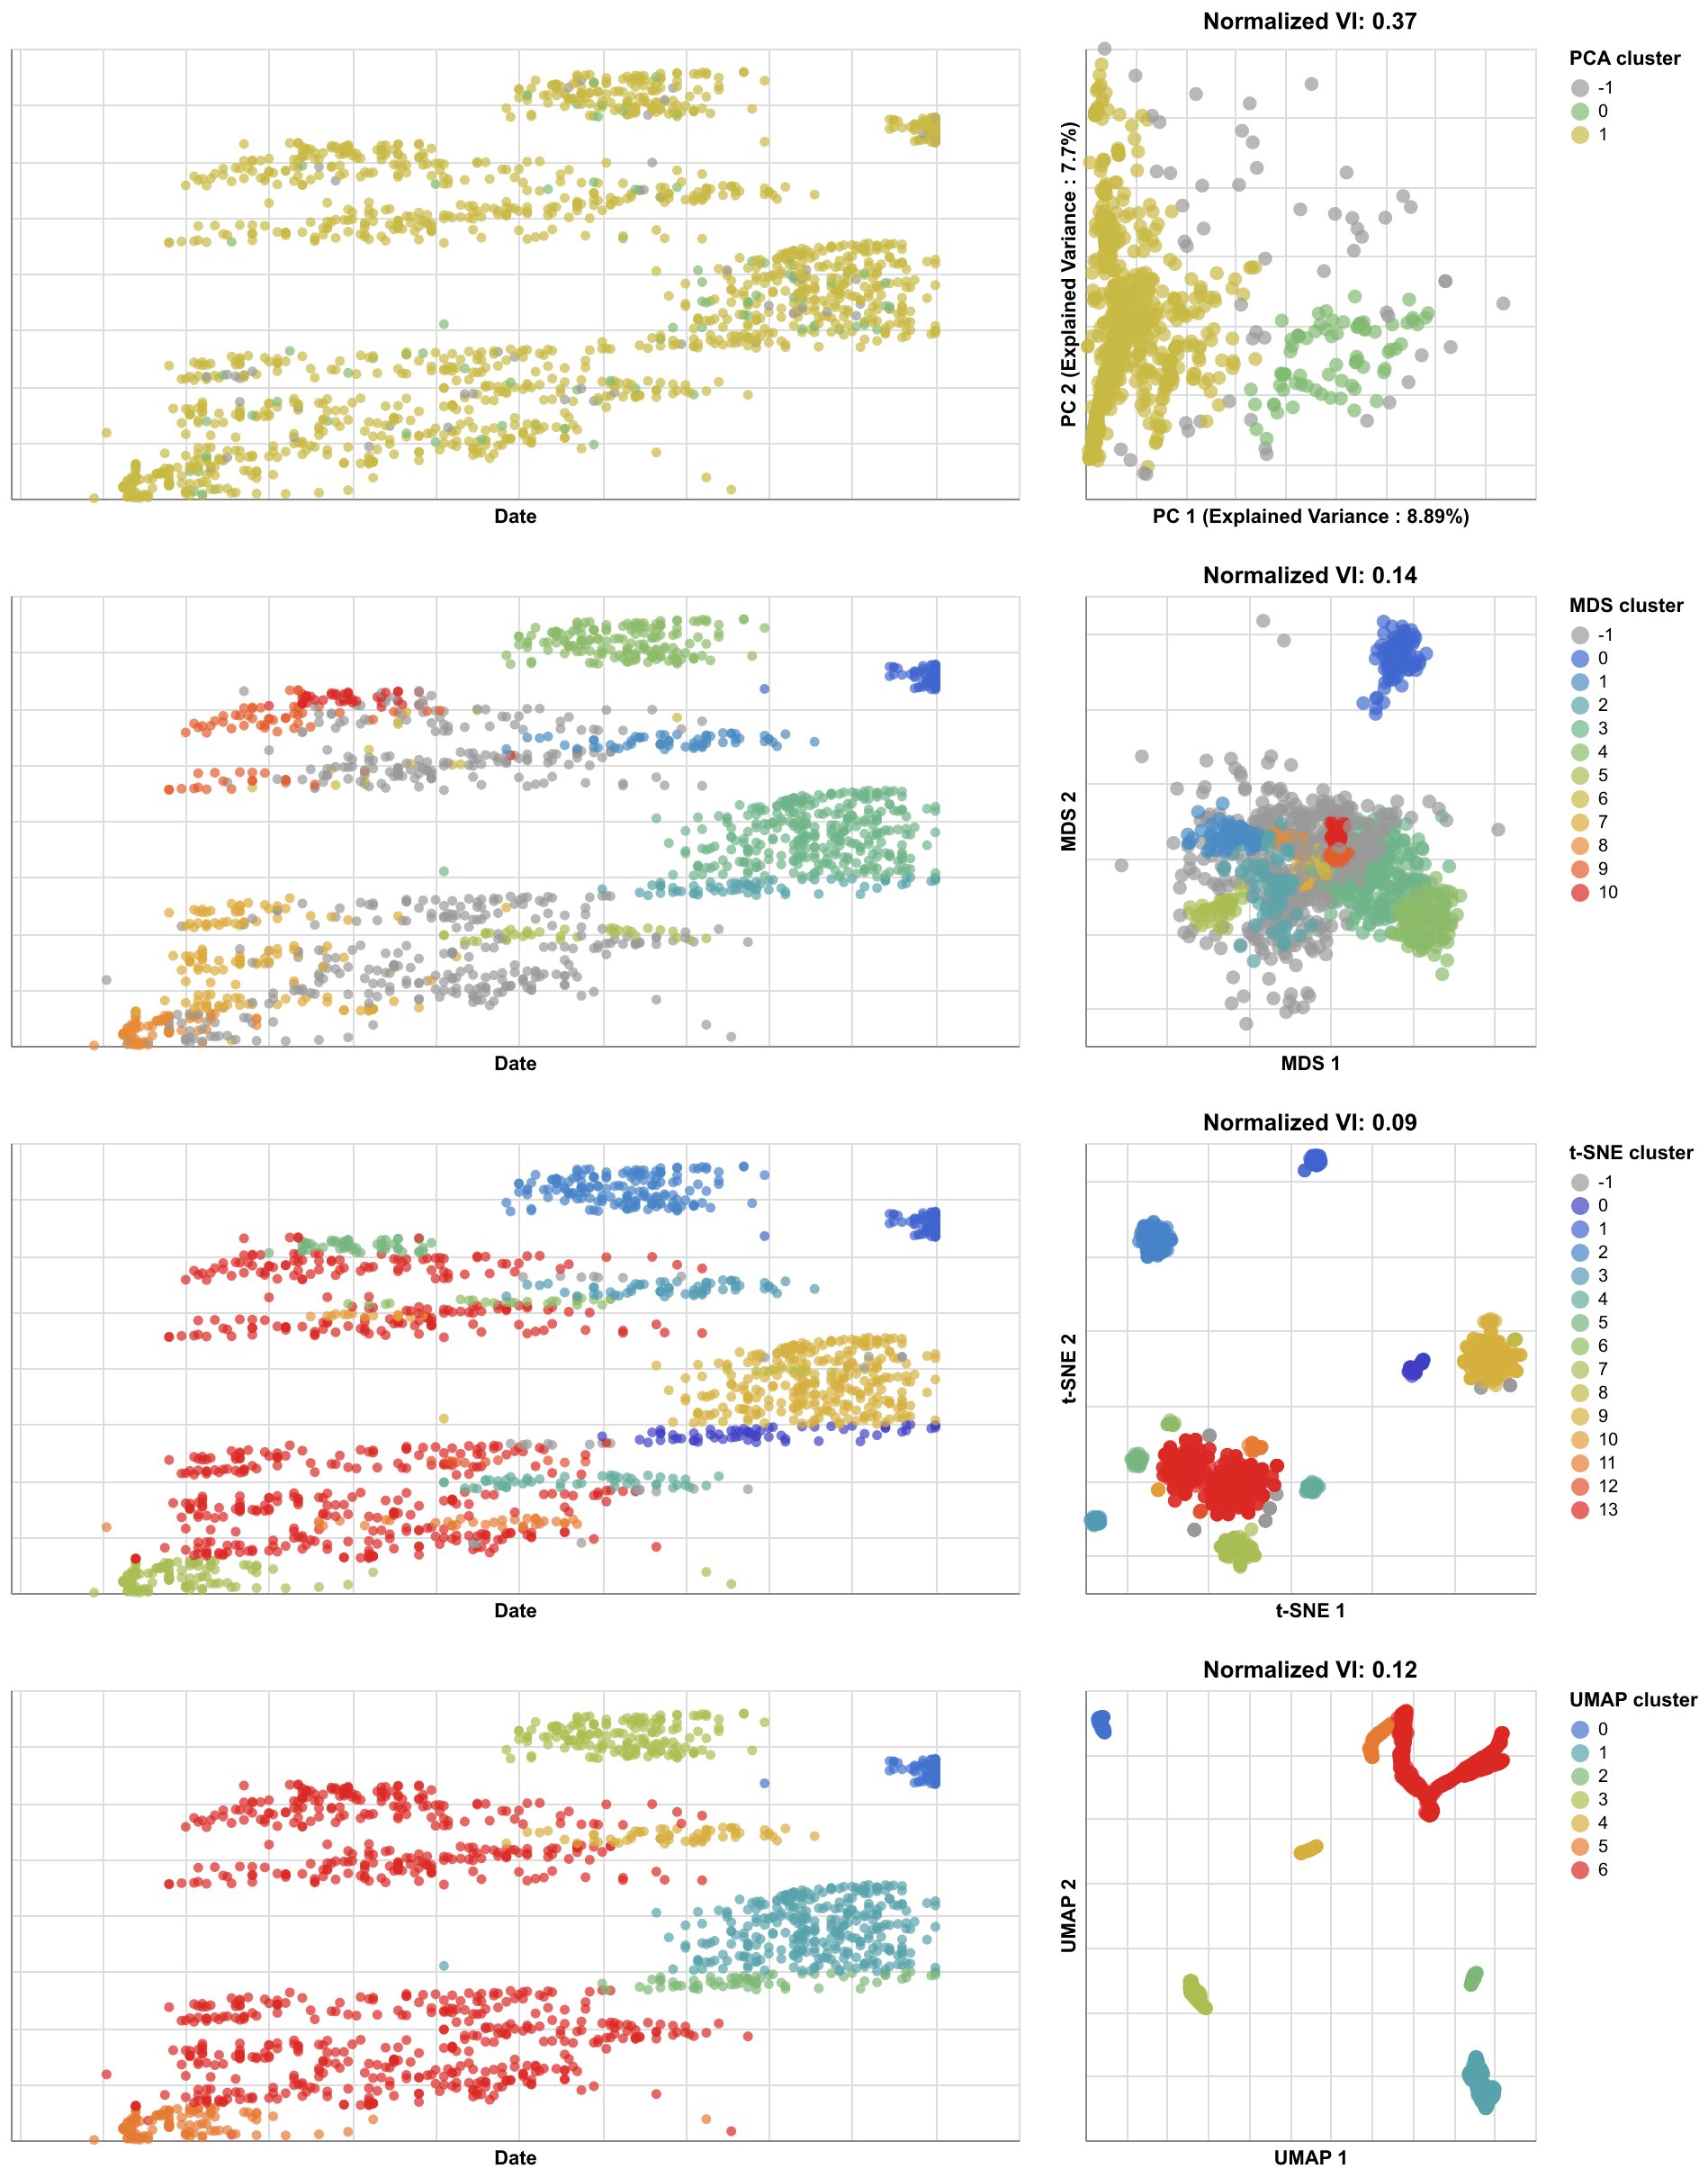
\includegraphics[width=\columnwidth]{figures/sarscov2-embeddings-by-cluster-vs-Nextstrain_clade.png}
\caption{{\bf Embeddings of SARS-CoV-2 sequences collected between January 1, 2020 and January 1, 2022 colored by embedding cluster and annotated by normalized VI to indicate accuracy of clusters for training data compared to expert clade assignment (Nextstrain clade).}
}
\label{fig:sars-cov-2-2020-2022-clusters-vs-Nextstrain-clade}
\end{figure}

\begin{figure}[!h]
% TODO: remove includegraphics commands in final submission; figures must be uploaded separately from the manuscript.
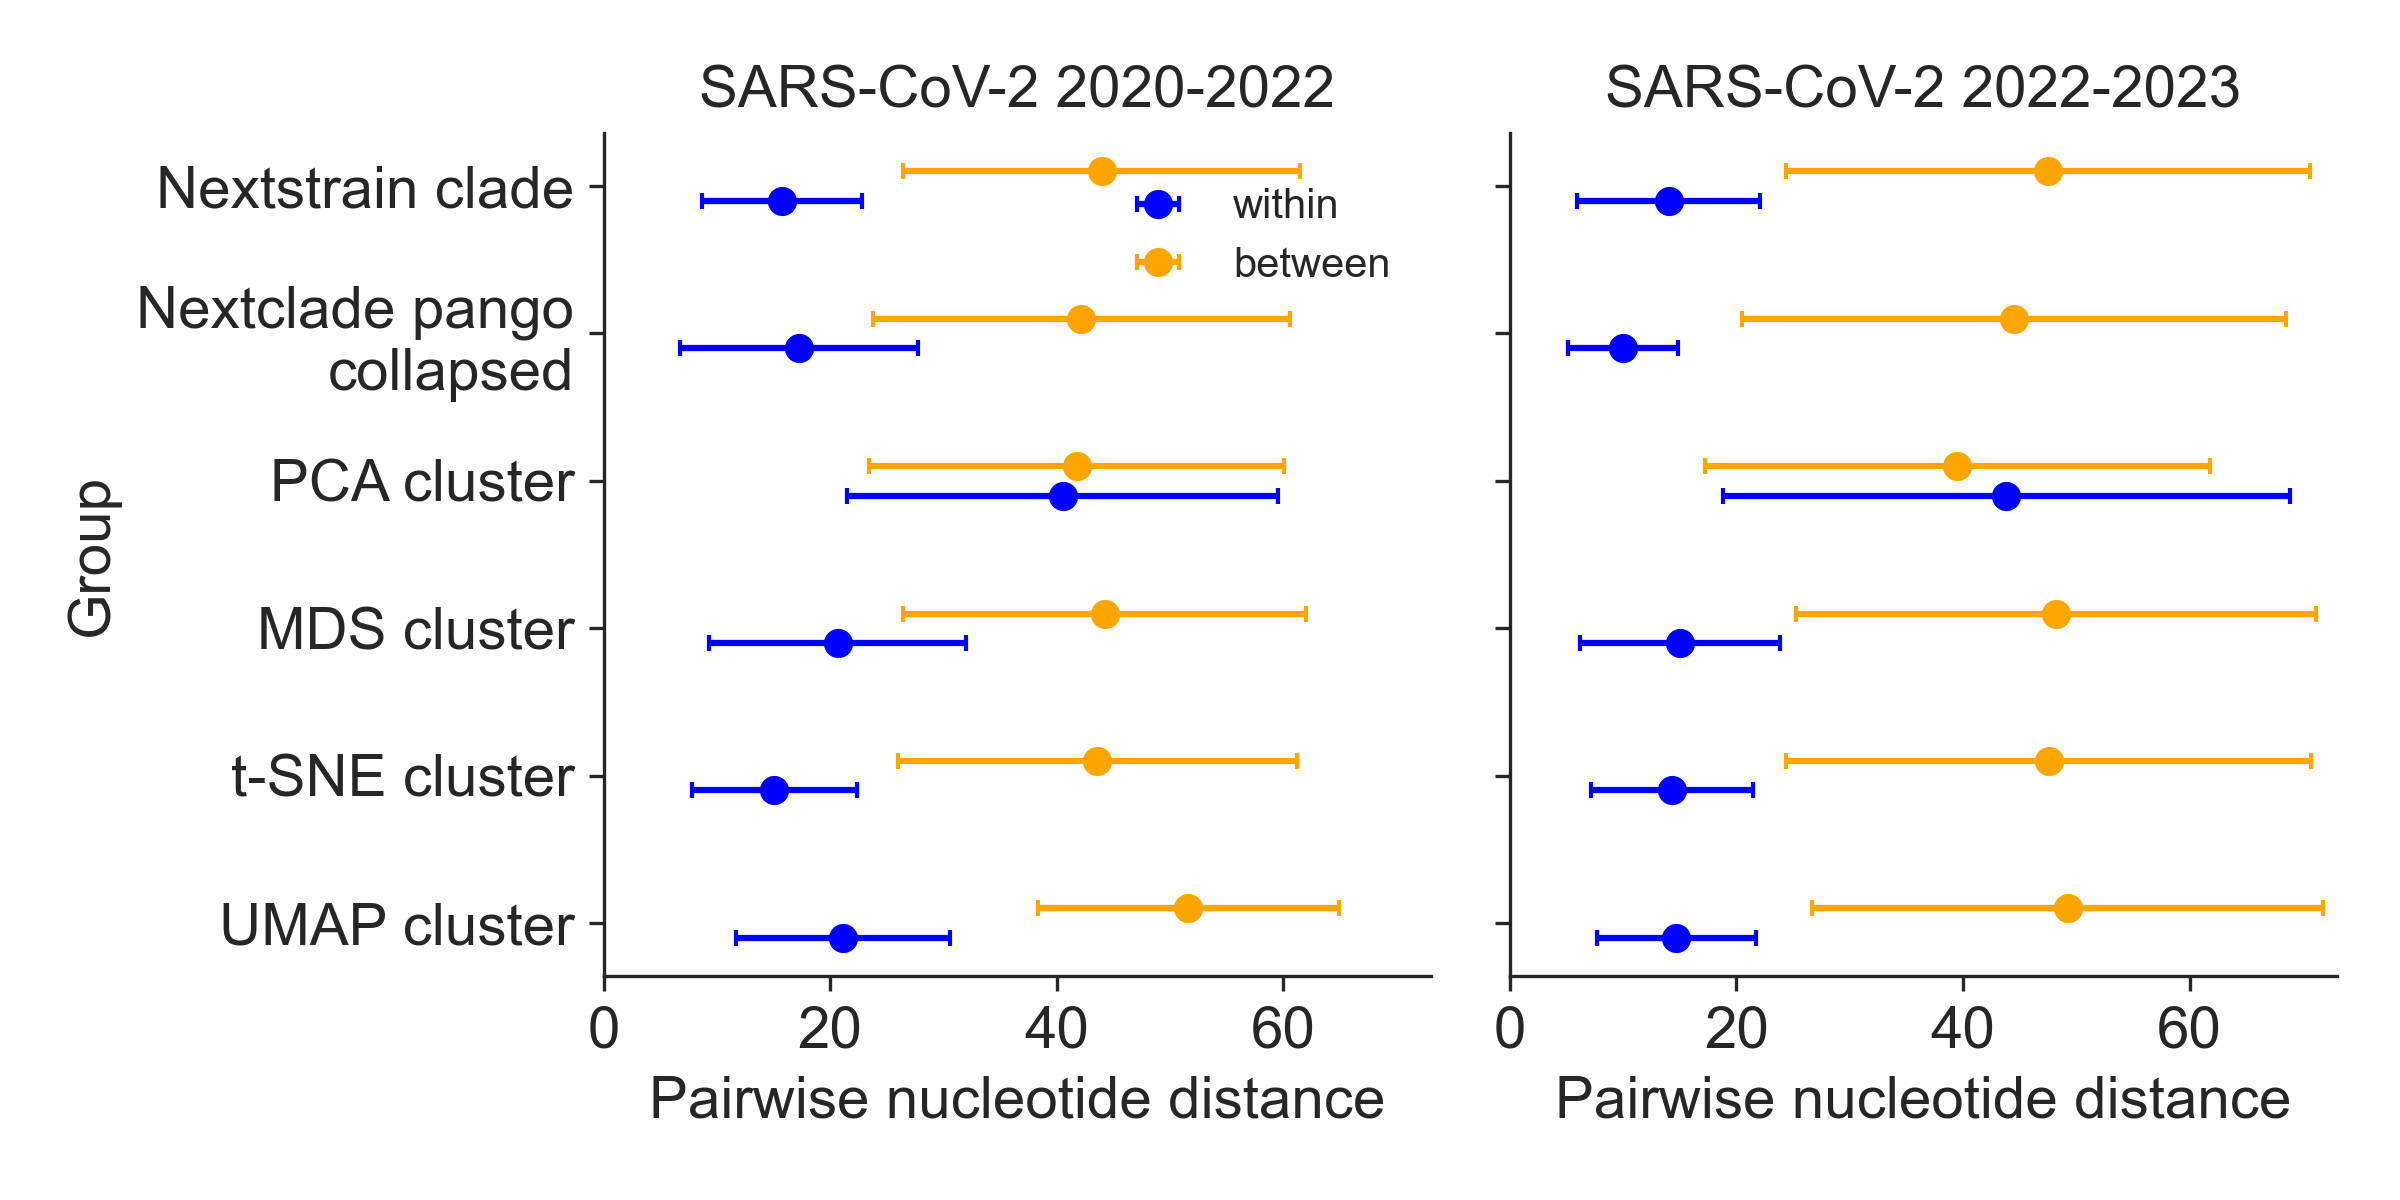
\includegraphics[width=\columnwidth]{figures/within_between_sars.png}
\caption*{{\bf S16 Fig. Pairwise nucleotide distances for early (2020-2022) and late (2022-2023) SARS-CoV-2 sequences within and between genetic groups defined by Nextstrain clades, collapsed Nextclade pango lineages, and clusters from PCA, MDS, t-SNE, and UMAP embeddings.}}
\end{figure}

When comparing clusters to Nextclade pango lineages, all four methods produced less accurate clusters (\nameref{S17_Fig_sarscov2_early_embeddings_by_cluster_vs_Nextclade_pango}).
Clusters from t-SNE were the most accurate with a VI of 0.17.
MDS and UMAP clusters performed similarly with VIs of 0.24 and 0.26.
PCA clusters remained the least accurate with a VI of 0.46.
The optimal minimum distances for three of the four methods remained the same, with only t-SNE's value changing from 1.5 to 1.0.
These results confirm quantitatively that these embeddings methods can accurately capture broader genetic diversity of SARS-CoV-2, but they cannot distinguish between fine resolution genetic groups identified by Pangolin.
However, we observed greater pairwise genetic distances within collapsed Nextclade pango lineages than within Nextstrain clades, suggesting that Pangolin lineages were not as tightly scoped as we originally expected (\nameref{S16_Fig_sarscov2_within_between_group_distances}).

\begin{figure}[!h]
% TODO: remove includegraphics commands in final submission; figures must be uploaded separately from the manuscript.
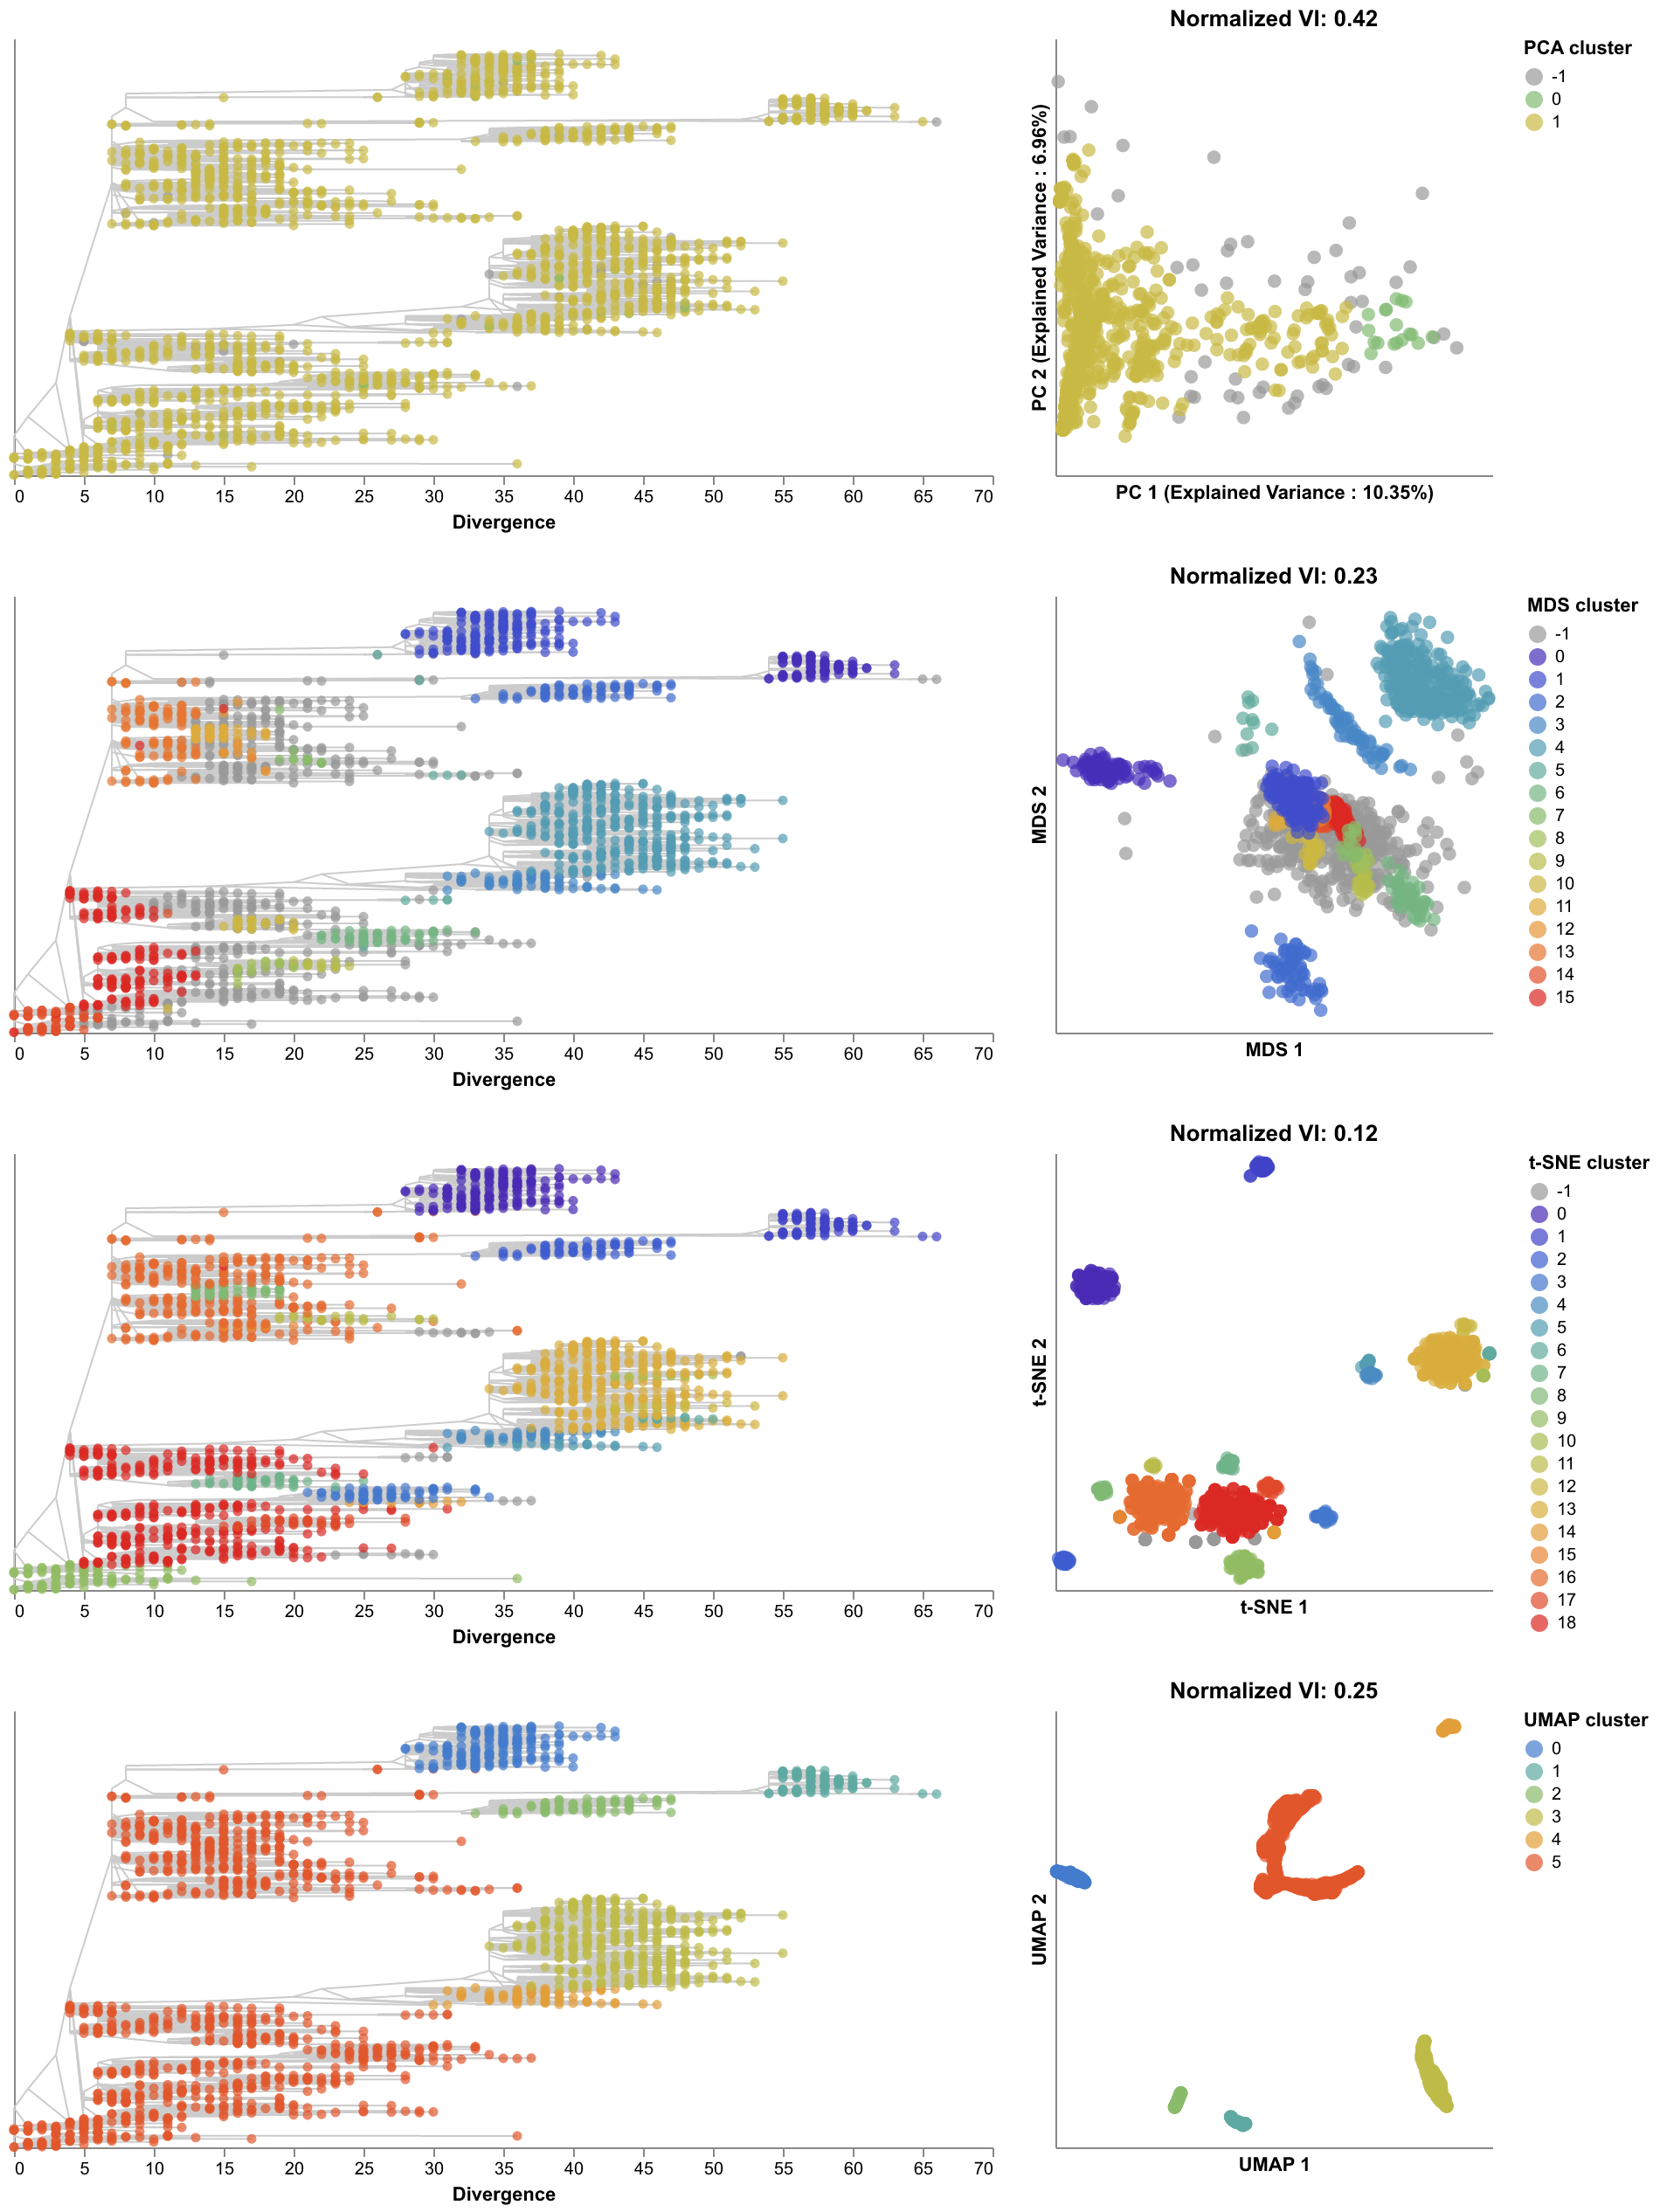
\includegraphics[width=\columnwidth]{figures/sarscov2-embeddings-by-cluster-vs-Nextclade_pango_collapsed.png}
\caption*{{\bf S17 Fig. Embeddings of SARS-CoV-2 sequences collected between January 1, 2020 and January 1, 2022 colored by embedding cluster and annotated by normalized VI to indicate accuracy of clusters for training data compared to expert clade assignment (collapsed Nextclade pango lineage).}}
\end{figure}

To test the optimal cluster parameters identified above, we applied embedding methods to late SARS-CoV-2 data and compared clusters from these embeddings to known genetic groups.
Of the 15 Nextstrain clades defined during this time period, 10 (67\%) descended from Omicron and represented 1,363 (93\%) of all samples in the dataset.
Of the 46 Nextclade pango lineages, 15 originated from a recombination event and corresponded to 380 (26\%) of all samples.
The clusters from embeddings of these more recent SARS-CoV-2 sequences performed as well or better than the clusters from earlier SARS-CoV-2 sequences (Fig.~\ref{fig:sars-cov-2-2022-2023-clusters-vs-Nextstrain-clade}).
UMAP clusters most accurately matched Nextstrain clades (normalized VI=0.07) with 10 clusters.
Clusters from t-SNE followed closely (normalized VI=0.08) with 17 clusters and MDS produced 11 clusters (normalized VI=0.13).
We found 23 cluster-specific mutations for two of six PCA clusters, 84 for eight of 11 MDS clusters, 107 for eight of 17 t-SNE clusters, and 125 for eight of 10 UMAP clusters (\nameref{S1_Table}).
Clusters from t-SNE remained the most consistently accurate across different random samples of sequences from the same time period and different total samples (\nameref{S18_Fig_late_sarscov2_replication_of_cluster_accuracy}).
UMAP clusters became more accurate and less variable as we added more sequences per group to the embeddings.

\begin{figure}[!h]
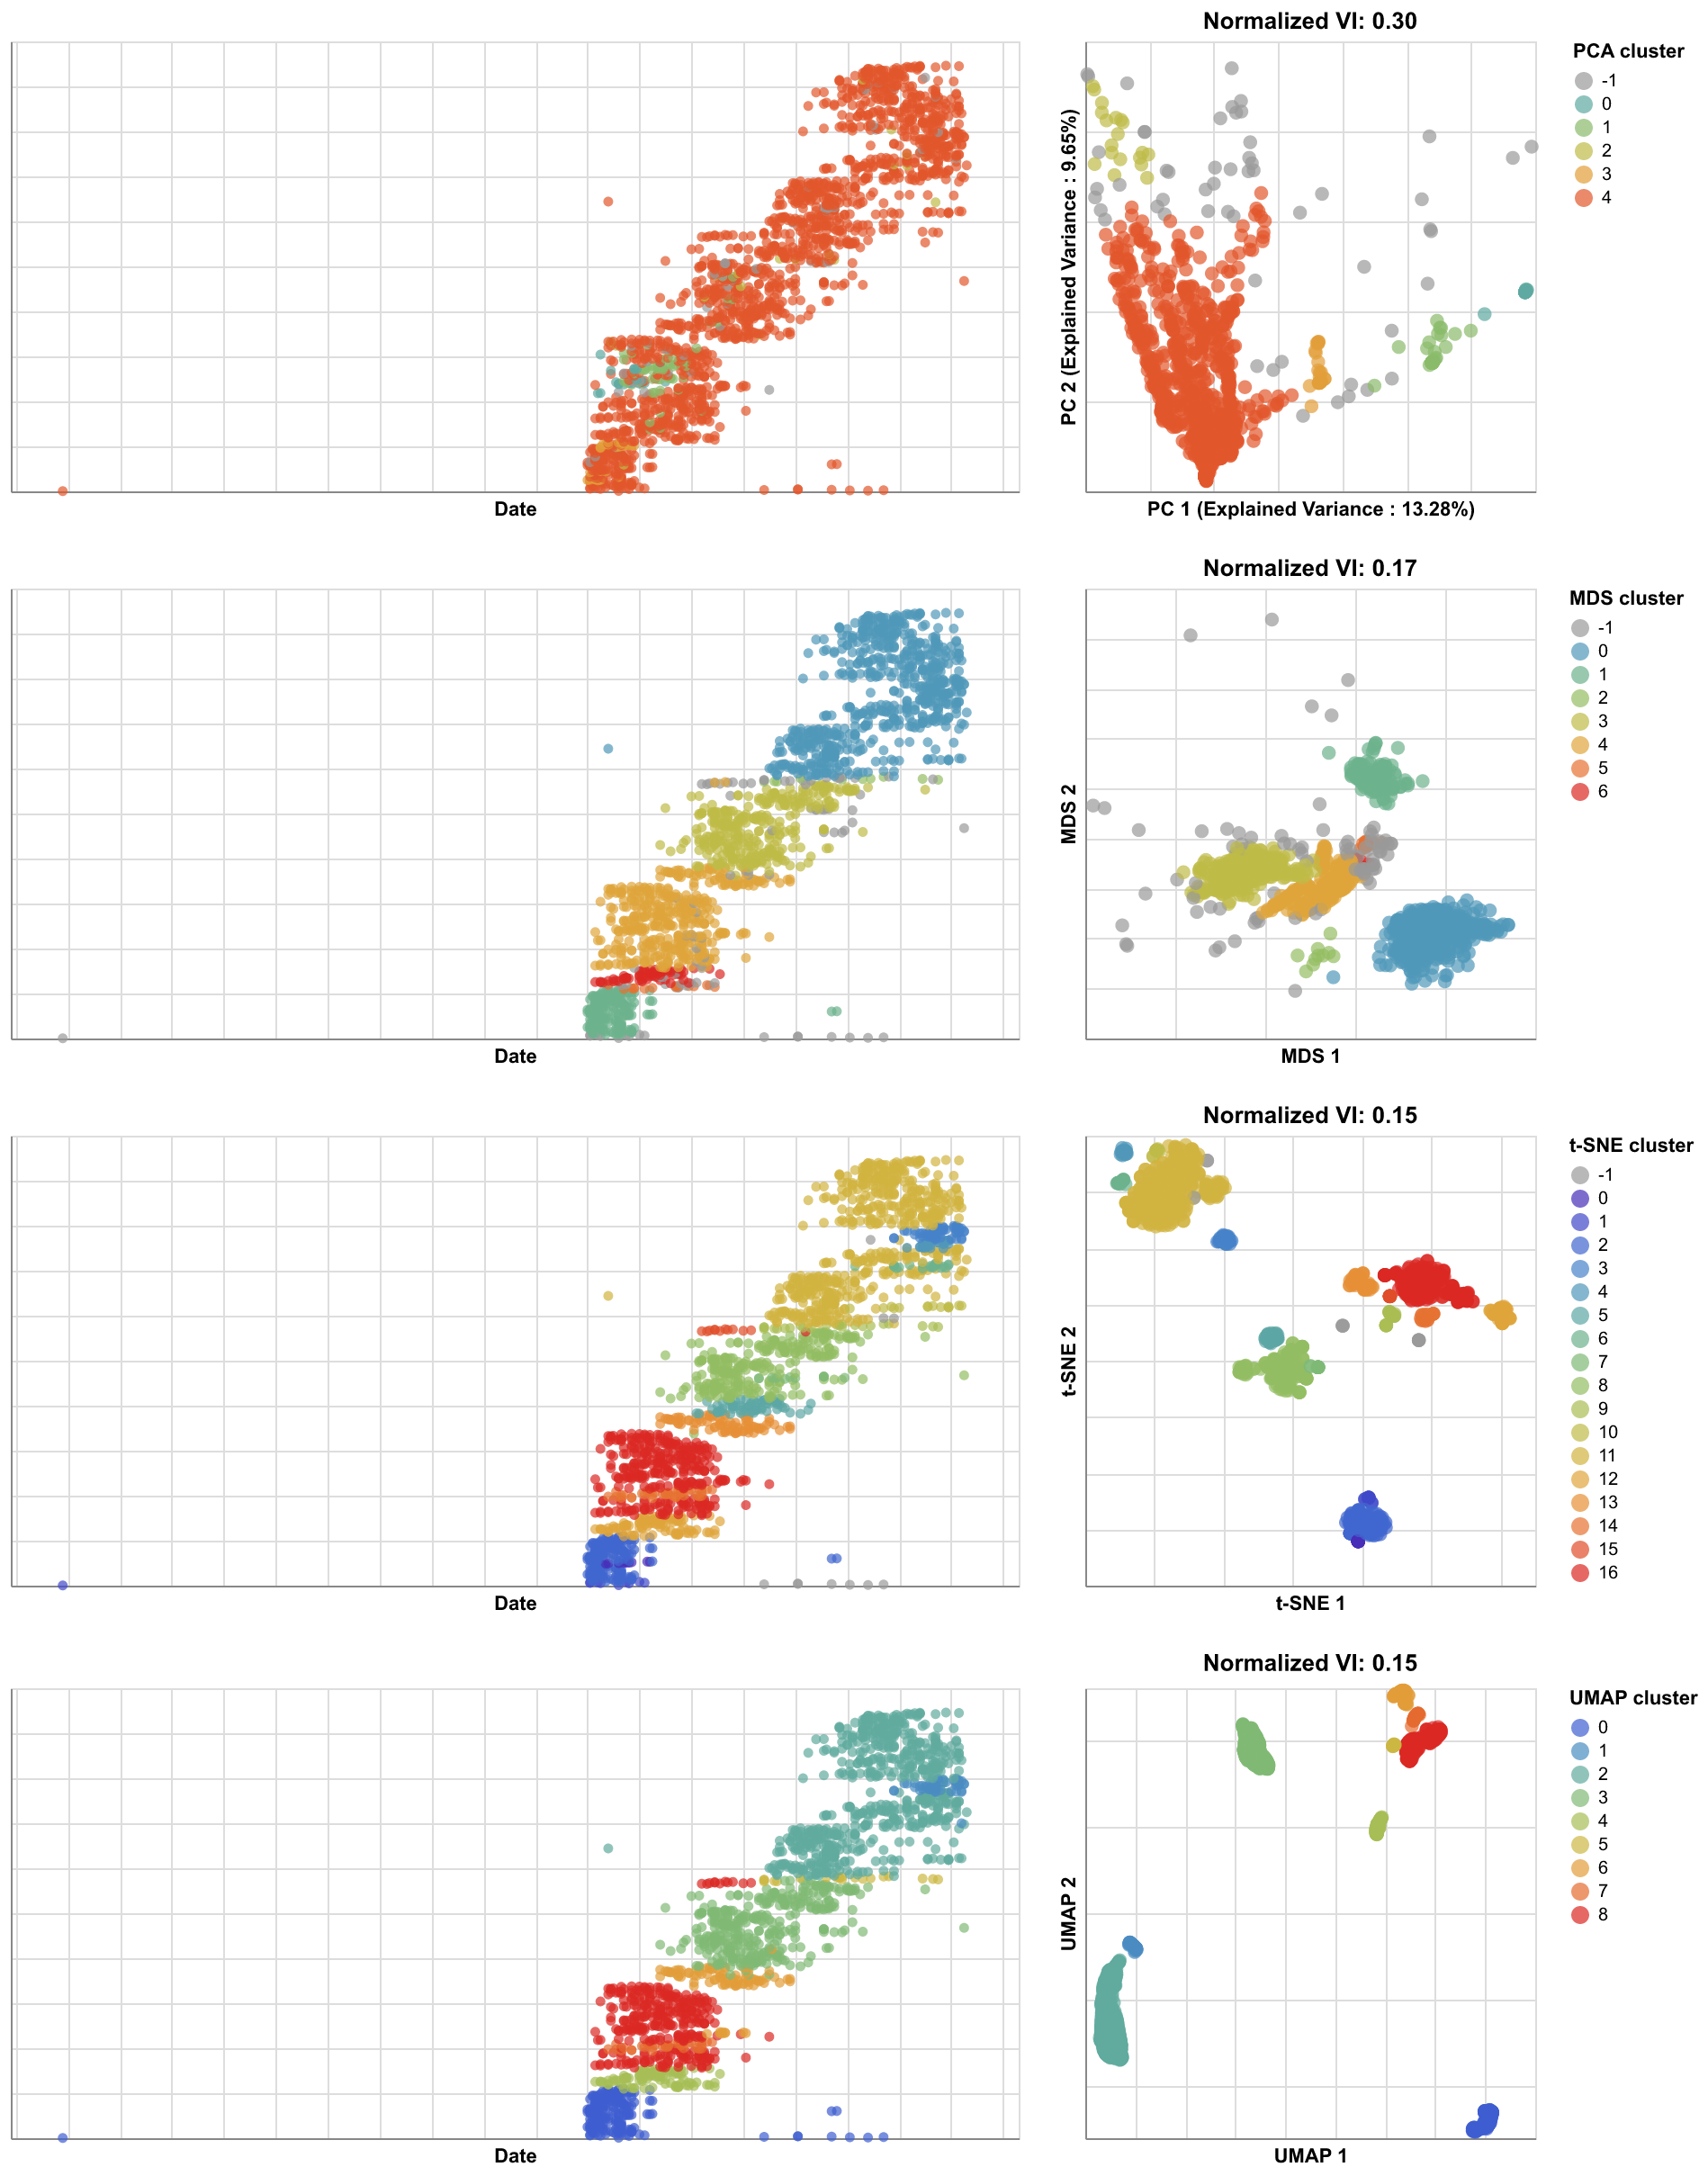
\includegraphics[width=\columnwidth]{figures/sarscov2-test-embeddings-by-cluster-vs-Nextstrain_clade.png}
\caption{{\bf Embeddings of SARS-CoV-2 sequences collected between January 1, 2022 and November 3, 2023 colored by embedding cluster and annotated by normalized VI to indicate accuracy of clusters for training data compared to expert clade assignment (Nextstrain clade).}
}
\label{fig:sars-cov-2-2022-2023-clusters-vs-Nextstrain-clade}
\end{figure}

\begin{figure}[!h]
% TODO: remove includegraphics commands in final submission; figures must be uploaded separately from the manuscript.
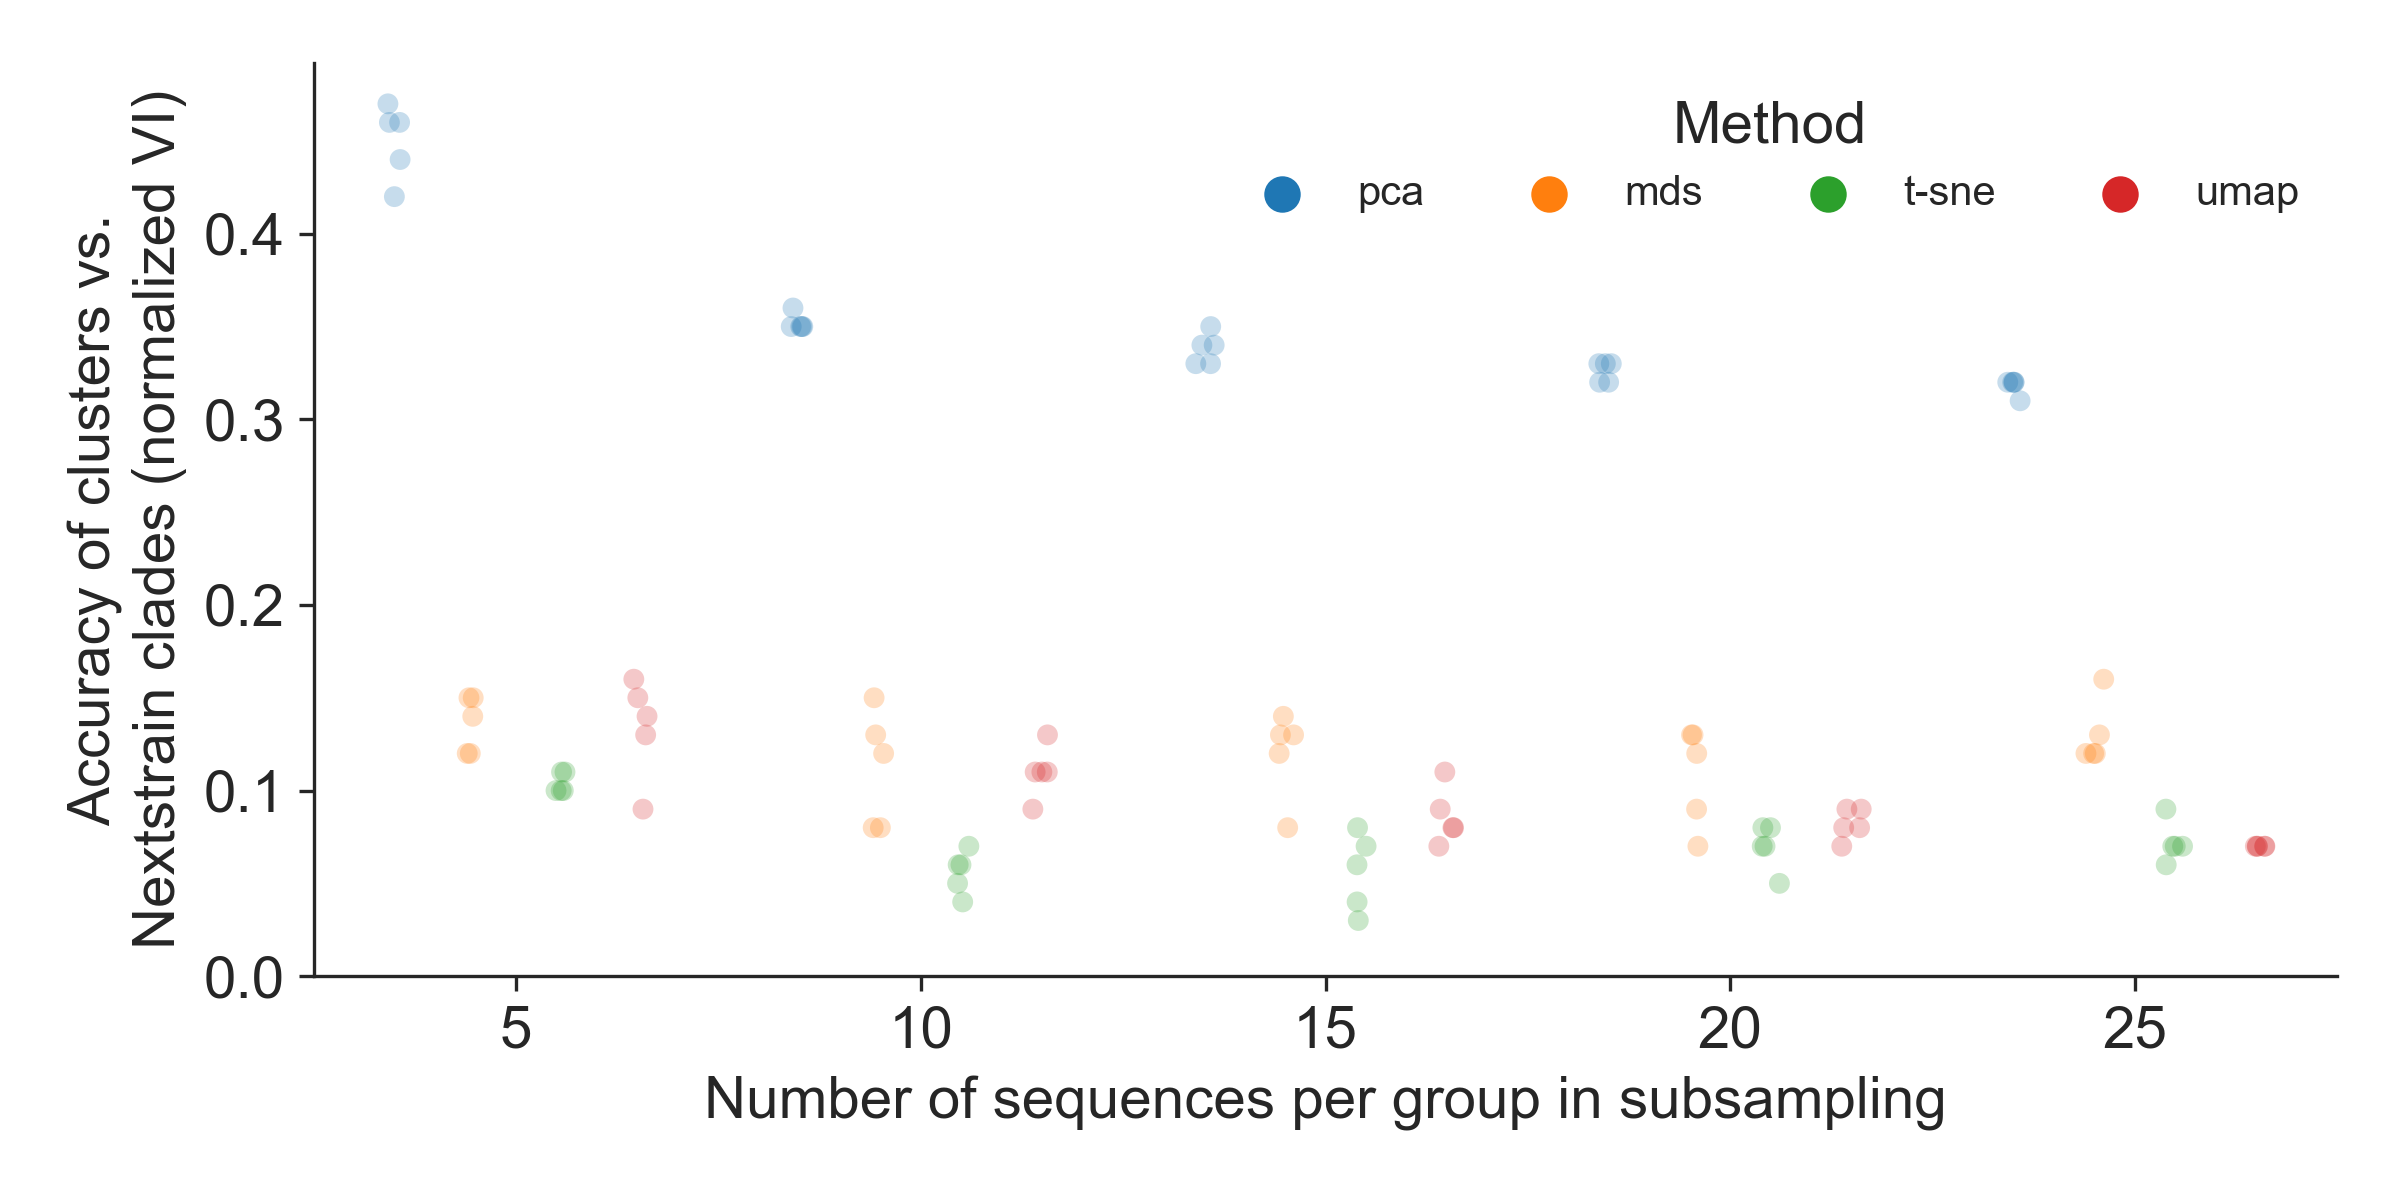
\includegraphics[width=\columnwidth]{figures/sarscov2-test-replication-of-cluster-accuracy.png}
\caption*{{\bf S18 Fig. Replication of cluster accuracy per embedding method for late (2022--2023) SARS-CoV-2 sequences across different sequences per group sampled from the original dataset and five replicates per sampling density.}}
\end{figure}

These three methods produced less accurate representations of Nextclade pango lineages (\nameref{S19_Fig_sarscov2_late_embeddings_by_cluster_vs_Nextclade_pango}).
UMAP's 10 clusters were three times farther from pango lineages than Nextstrain clades (normalized VI=0.21).
Clusters from MDS (N=11) and t-SNE (N=27) were twice as far from pango lineages as Nextstrain clades (normalized VI=0.28 and 0.14, respectively).
These results replicate the patterns we observed with early SARS-CoV-2 data where clusters from embeddings more effectively represented broader genetic diversity than the finer resolution diversity labeled by Pangolin.
Unlike the Nextclade pango lineages in the early SARS-CoV-2 data, the lineages from the later data exhibited fewer pairwise genetic distances between samples in each lineage than samples in Nextstrain clades or any embedding cluster (\nameref{S16_Fig_sarscov2_within_between_group_distances}).

\begin{figure}[!h]
% TODO: remove includegraphics commands in final submission; figures must be uploaded separately from the manuscript.
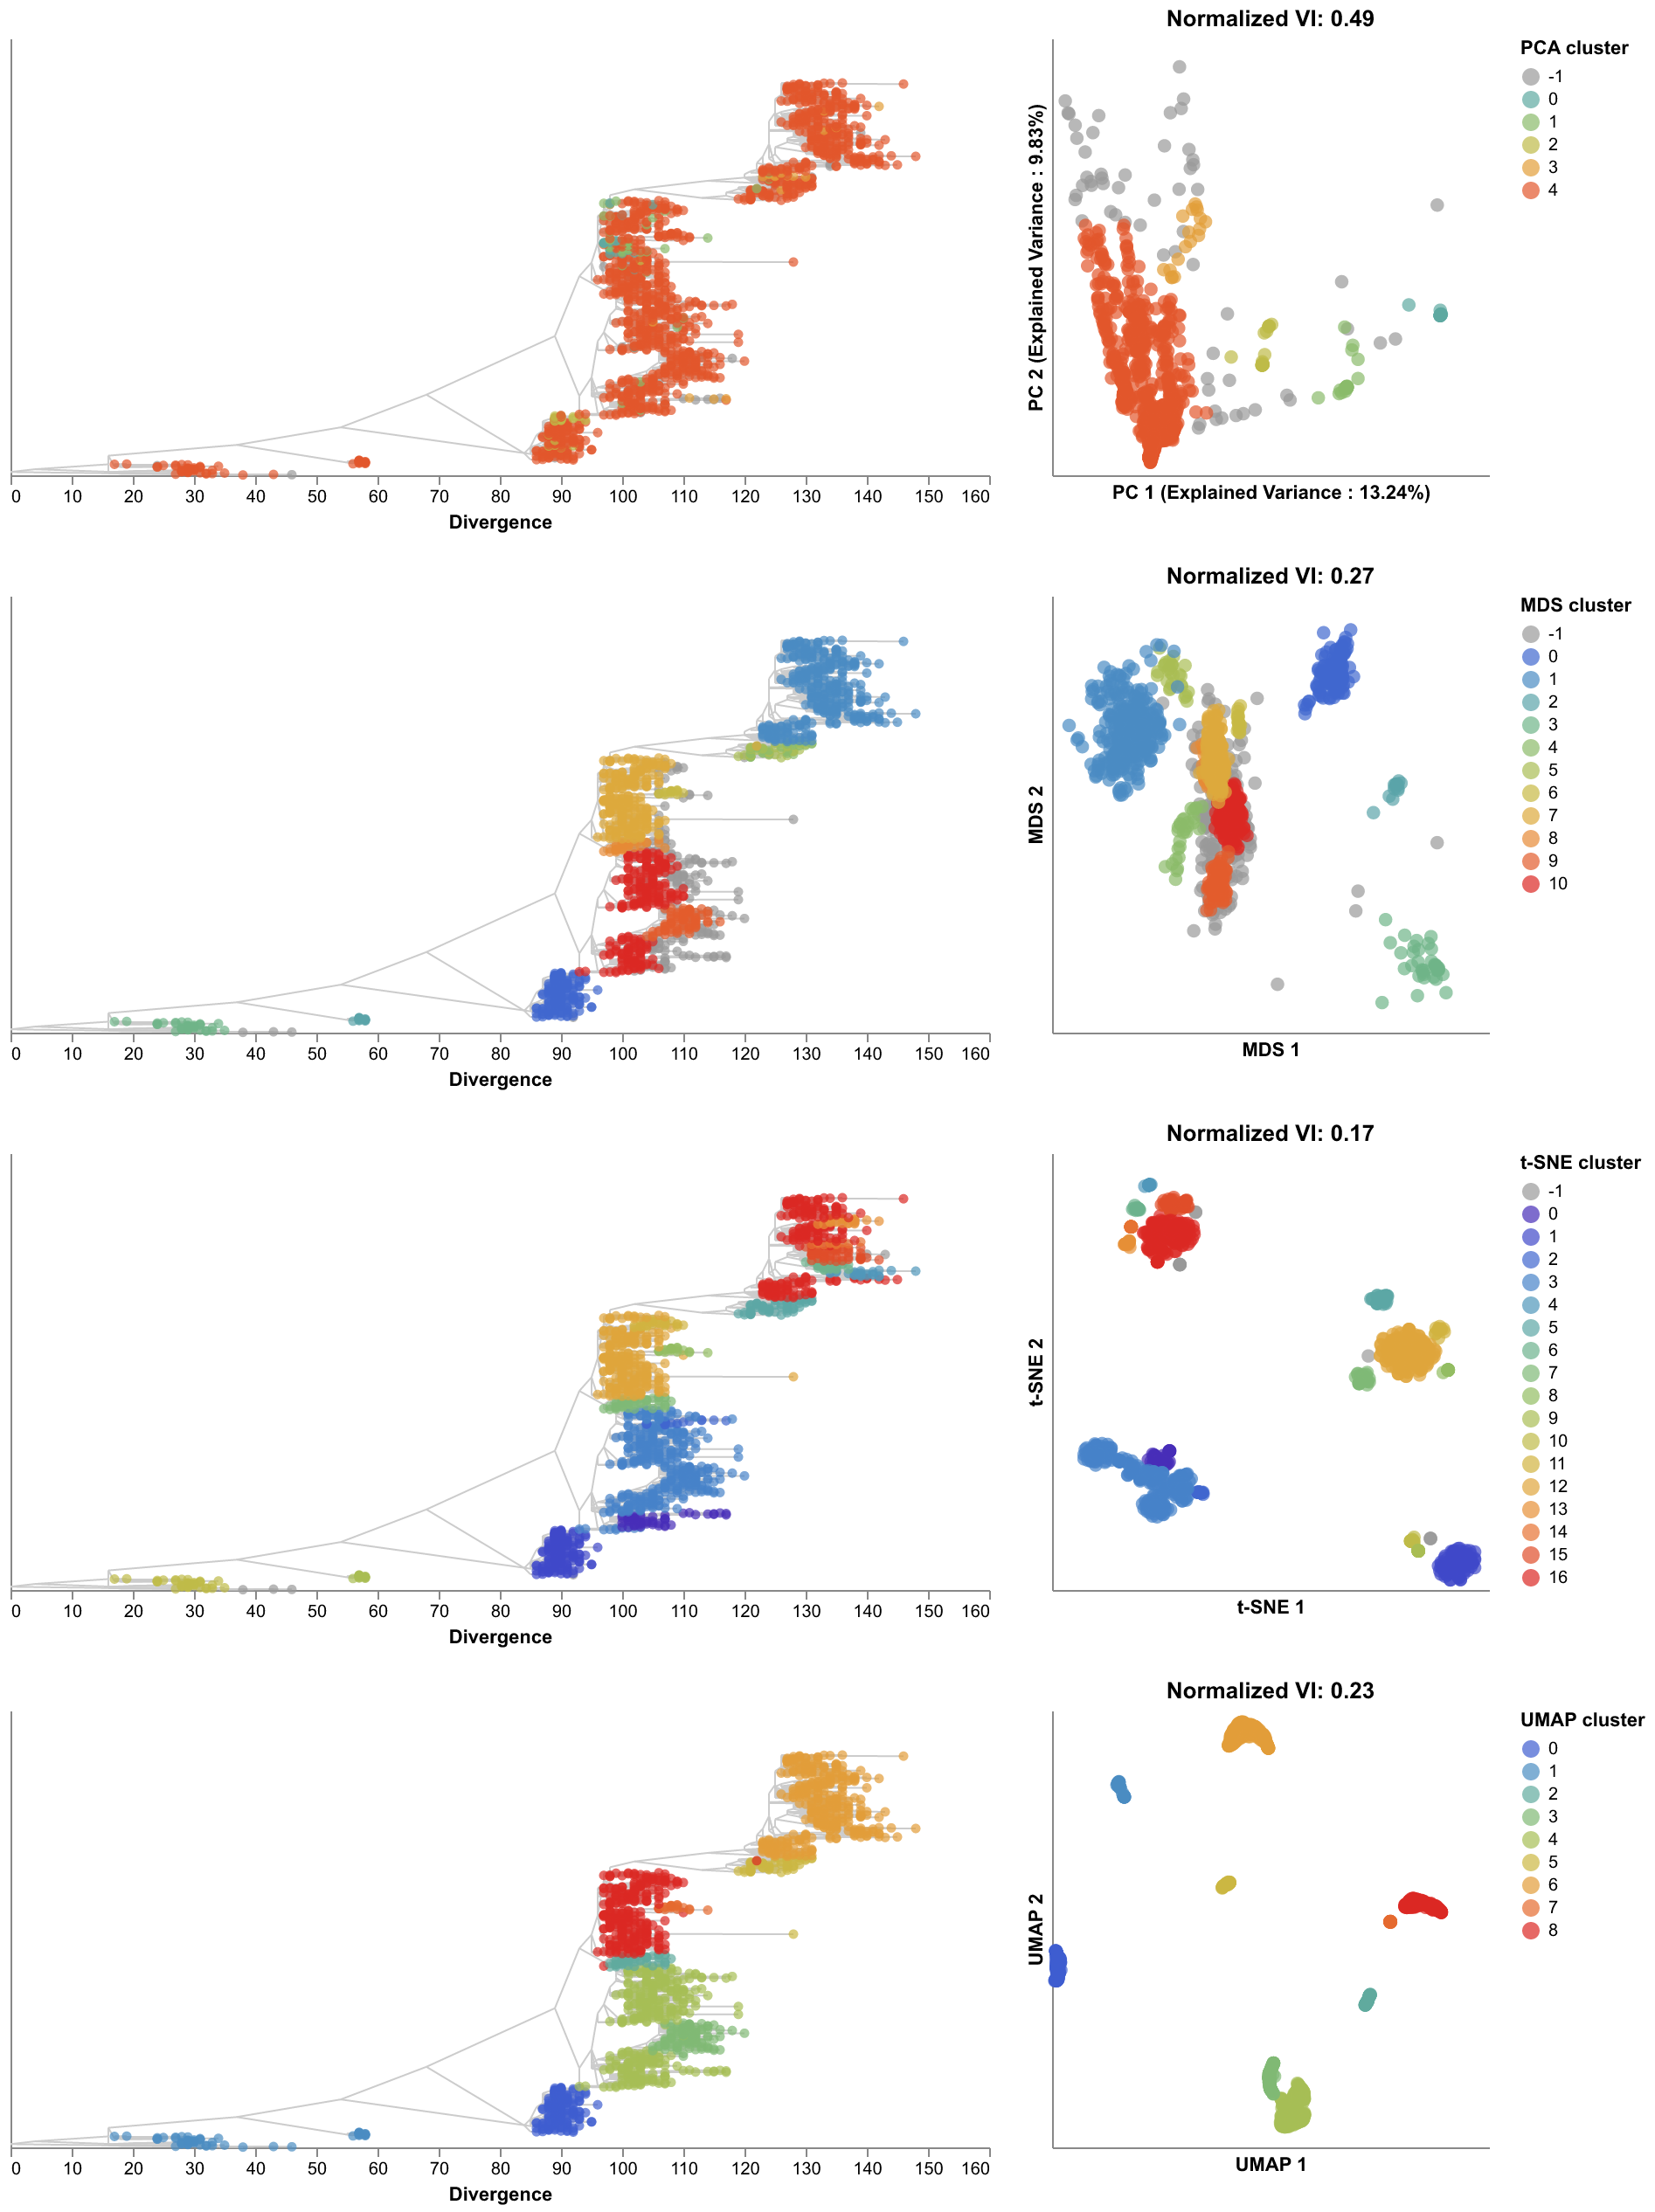
\includegraphics[width=\columnwidth]{figures/sarscov2-test-embeddings-by-cluster-vs-Nextclade_pango_collapsed.png}
\caption*{{\bf S19 Fig. Embeddings of SARS-CoV-2 sequences collected between January 1, 2022 and November 3, 2023 colored by embedding cluster and annotated by normalized VI to indicate accuracy of clusters for training data compared to expert clade assignment (collapsed Nextclade pango lineage).}}
\end{figure}

\subsection*{Distance-based embeddings reflect SARS-CoV-2 recombination events}

Finally, we tested the ability of sequence embeddings to capture patterns of recombination between known parental lineages of SARS-CoV-2.
We reasoned that each recombinant lineage, $X$, should always place closer to its parental lineages $A$ and $B$ than the parental lineages place to each other.
Based on this logic, we calculated the average Euclidean distance between pairs of samples in lineages $A$ and $B$, $A$ and $X$, and $B$ and $X$ for each embedding method (see Methods).
We identified recombinant lineages that mapped closer to both of their parental lineages and those that mapped closer to at least one of the parental lineages.

Only five of the ten recombinant lineages that we inspected had enough samples in both parental and recombinant lineages to calculate average pairwise distances (XD, XE, XG, XBB, and XBL).
MDS embeddings most consistently reflected recombination events with four of five (80\%) recombinant lineages mapping closer to both parental lineages (\nameref{S2_Table}).
Three (60\%) recombinant lineages mapped between parents in t-SNE embeddings and only two (40\%) mapped between parentals in PCA and UMAP.
However, all recombinant lineages mapped closer to at least one parent in all embeddings.

% Place tables after the first paragraph in which they are cited.
\begin{table}[!ht]
%\begin{adjustwidth}{-2.25in}{0in} % Comment out/remove adjustwidth environment if table fits in text column.
\centering
\caption*{
  {\bf S2 Table. Average Euclidean distances between each known recombinant, ``X'', and its parental lineages ``A'' and ``B'' per embedding method.}
  Distances include average pairwise comparisons between A and B, A and X, and B and X.
  Additional columns indicate whether each recombinant lineage maps closer to both parental lineages (or at least one) than those parents map to each other.}
\scalebox{0.5}{
  \begin{tabular}{llllrrrll}
\toprule
parental\_A & parental\_B & recombinant\_X & method &  distance\_A\_B &  distance\_A\_X &  distance\_B\_X &  X\_maps\_closer\_to\_both\_parentals &  X\_maps\_closer\_to\_any\_parental \\
\midrule
      AY.4 &       BA.1 &            XD &    PCA &         16.00 &          8.55 &         16.45 &                            False &                           True \\
      BA.1 &       BA.2 &            XE &    PCA &         34.40 &         31.56 &         42.59 &                            False &                           True \\
      BA.1 &       BA.2 &            XG &    PCA &         34.40 &         15.29 &         30.68 &                             True &                           True \\
      BJ.1 &   BM.1.1.1 &           XBB &    PCA &         21.42 &         18.51 &         19.86 &                             True &                           True \\
     XBB.1 &    BA.2.75 &           XBL &    PCA &         16.08 &         18.35 &         15.14 &                            False &                           True \\
      AY.4 &       BA.1 &            XD &    MDS &         76.79 &         36.95 &         51.18 &                             True &                           True \\
      BA.1 &       BA.2 &            XE &    MDS &         47.09 &         28.56 &         21.83 &                             True &                           True \\
      BA.1 &       BA.2 &            XG &    MDS &         47.09 &         35.62 &         14.77 &                             True &                           True \\
      BJ.1 &   BM.1.1.1 &           XBB &    MDS &         33.58 &         20.03 &         29.37 &                             True &                           True \\
     XBB.1 &    BA.2.75 &           XBL &    MDS &         28.25 &         14.73 &         35.81 &                            False &                           True \\
      AY.4 &       BA.1 &            XD &  t-SNE &          6.06 &          1.56 &          4.69 &                             True &                           True \\
      BA.1 &       BA.2 &            XE &  t-SNE &         32.91 &         32.86 &          5.33 &                             True &                           True \\
      BA.1 &       BA.2 &            XG &  t-SNE &         32.91 &         34.07 &          5.66 &                            False &                           True \\
      BJ.1 &   BM.1.1.1 &           XBB &  t-SNE &         25.86 &          6.77 &         31.03 &                            False &                           True \\
     XBB.1 &    BA.2.75 &           XBL &  t-SNE &         30.23 &          6.07 &         24.58 &                             True &                           True \\
      AY.4 &       BA.1 &            XD &   UMAP &         11.79 &          1.01 &         11.04 &                             True &                           True \\
      BA.1 &       BA.2 &            XE &   UMAP &         17.36 &         17.71 &          3.49 &                            False &                           True \\
      BA.1 &       BA.2 &            XG &   UMAP &         17.36 &         17.83 &          3.67 &                            False &                           True \\
      BJ.1 &   BM.1.1.1 &           XBB &   UMAP &         20.04 &          1.04 &         20.31 &                            False &                           True \\
     XBB.1 &    BA.2.75 &           XBL &   UMAP &         20.90 &          2.06 &         19.94 &                             True &                           True \\
\bottomrule
\end{tabular}

}
%\end{adjustwidth}
\end{table}

\section*{Discussion}

% What we learned and pros of methods
We applied four standard dimensionality reduction methods to simulated and natural genome sequences of two relevant human pathogenic viruses and found that the resulting embeddings could reflect pairwise genetic relationships between samples and capture previously identified genetic groups.
From our analysis of simulated influenza- and coronavirus-like sequences, we found that each method produced consistent embeddings of genetic sequences for two distinct pathogens, more than 55 years of evolution, and a wide range of practical method parameters.
These results suggest that researchers could apply these biologically-uninformed methods to a broad range of human pathogenic viruses with minimal tuning of the method parameters.
Of the four methods, MDS most accurately reflected pairwise genetic distances between simulated samples in its embeddings.
From our analysis of natural populations of seasonal influenza H3N2 HA and SARS-CoV-2 sequences, we confirmed that MDS most reliably reflected pairwise genetic distances and we found that clusters from t-SNE and UMAP embeddings most accurately recapitulated previously defined genetic groups at the resolution of WHO and Nextstrain clades.
Clusters from t-SNE embeddings of H3N2 HA and NA sequences accurately matched reassortment clades identified by a biologically-informed model based on ancestral reassortment graphs.
MDS embeddings placed known recombinant lineages of SARS-CoV-2 between their parental lineages.
From these results, we conclude that tree-free dimensionality reduction methods can provide valuable biological insights for human pathogenic viruses through easily interpretable visualizations of genetic relationships and the ability to account for genetic variation that phylogenetic methods cannot including indels, reassortment, and recombination.

% Limitations of methods and analysis
Despite the promise of these simple methods to answer important public health questions about human pathogenic viruses, these methods and our analyses suffer from inherent limitations.
The lack of an underlying biological model is both a strength and the clearest limitation of the dimensionality reduction methods we considered here.
For example, embeddings of SARS-CoV-2 genomes cannot capture the same fine-grained genetic resolution as Pangolin lineage annotations.
Each method provides only a few parameters to tune its embeddings and these parameters have little effect on the qualitative outcome.
Each method also suffers from specific issues in our analysis.
PCA performs poorly with missing data and requires researchers to impute the missing values prior to analysis, as previously shown for Zika virus \cite{metsky_2017}.
Neither t-SNE nor UMAP maintain a linear relationship between pairwise Euclidean and genetic distances across the observed range of genetic distances.
As a result, viewers cannot know that samples mapping far apart in a t-SNE or UMAP embedding are as genetically distant as they appear.
In maintaining a linear relationship between Euclidean and genetic distances, MDS sacrifices the ability to form more accurate genetic clusters.
Given these limitations of these methods, we do not expect them to replace biologically-informed methods that provide more meaningful parameters to tune their algorithms.
Instead, we expect that researchers can use these methods for rapid visualization and clustering of their genome sequences as the first step prior to analysis with more sophisticated and computationally intensive algorithms.

We note that our analysis reflects a small subset of human pathogen viruses and dimensionality reduction methods.
We focused on analysis of two respiratory RNA viruses that contribute dramatically to seasonal human morbidity and mortality, but numerous alternative pathogens would also have been relevant subjects.
For example, HIV represents a canonical example of a highly recombinant and bloodborne virus, while Zika, dengue, and West Nile viruses represent pathogens with multiple host species in a transmission chain.
Similarly, we selected only four dimensionality reduction methods from myriad options that are commonly applied to genetic data \cite{Armstrong2022}.
We chose these methods based on their wide use and availability in tools like scikit-learn \cite{Pedregosa2011} and to limit the dimensionality of our analyses.
Finally, we chose to analyze a consistent, fixed number of sequences for each pathogen, but the nature of embeddings, their optimal parameters, and their computational efficiency may vary with input size.

% Future directions and use of methods
Some limitations noted above suggest future directions for this line of research.
We provide optimal settings for each pathogen and embedding method in this study and open source tools to apply these methods to other pathogens.
Researchers can easily integrate these tools into existing workflows for the genomic epidemiology of viruses and visualize the results with Nextstrain.
Alternately, researchers may choose to apply similar existing tools developed for metagenomic analysis \cite{Schloss2009,Schloss2020,Bolyen2019,McMurdie2013} to the analysis of viral populations.
In the short term, researchers can apply the methods we describe here to seasonal influenza and SARS-CoV-2 genomes to identify biologically relevant clusters including reassortment events or recombinant lineages.
In the long term, we expect researchers will benefit from expanding the breadth of dimensionality reduction methods applied to viruses and the breath of viral diversity assessed by these methods.

\section*{Conclusion}

We showed that simple dimensionality reduction methods operating on pairwise genetic differences can capture biologically-relevant clusters of phylogenetic clades, reassortment events, and patterns of recombining lineages for human pathogenic viruses.
The conceptual and practical simplicity of these tools should enable researchers to more readily visualize and compare samples for human pathogenic viruses when phylogenetic methods are either unnecessary or inappropriate.

\section*{Supporting information}

% Include only the SI item label in the paragraph heading. Use the \nameref{label} command to cite SI items in the text.
\paragraph*{S1 Fig.}
\label{S1_Fig_simulated_flu_errors}
{\bf Distribution of mean absolute errors (MAE) between observed and predicted pairwise genetic distances per embedding method parameters for simulated influenza-like populations.} Each panel shows boxplots of MAEs for a specific embedding method (PCA, MDS, t-SNE, and UMAP) and a given combination of method parameters. Boxplots reflect median, upper and lower quartiles, and the range of values.

\paragraph*{S2 Fig.}
\label{S2_Fig_simulated_coronavirus_errors}
{\bf Distribution of mean absolute errors (MAE) between observed and predicted pairwise genetic distances per embedding method parameters for simulated coronavirus-like populations.} Each panel shows boxplots of MAEs for a specific embedding method (PCA, MDS, t-SNE, and UMAP) and a given combination of method parameters. Boxplots reflect median, upper and lower quartiles, and the range of values.

\paragraph*{S3 Fig.}
\label{S3_Fig_simulated_representative_mds_embeddings}
{\bf Representative MDS embeddings for simulated populations using optimal parameters per pathogen (rows) and showing all three components.}

\paragraph*{S4 Fig.}
\label{S4_Fig_flu_within_between_group_distances}
{\bf Pairwise nucleotide distances for early (2016--2018) and late (2018--2020) influenza H3N2 HA sequences within and between genetic groups defined by Nextstrain clades and clusters from PCA, MDS, t-SNE, and UMAP embeddings.}

\paragraph*{S5 Fig.}
\label{S5_Fig_late_flu_embeddings_by_clade}
{\bf Phylogeny of late (2018--2020) influenza H3N2 HA sequences (top) and reduced dimensionality embeddings of genetic sequences into two dimensions by PCA (middle left), MDS (middle right), t-SNE (bottom left), and UMAP (bottom right).}

\paragraph*{S6 Fig.}
\label{S6_Fig_late_flu_mds_embeddings}
{\bf MDS embeddings for late (2018--2020) influenza H3N2 HA sequences showing all three components.}

\paragraph*{S7 Fig.}
\label{S7_Fig_late_flu_replication_of_cluster_accuracy}
{\bf Replication of cluster accuracy per embedding method for late (2018--2020) influenza H3N2 HA sequences across different sequences per group sampled from the original dataset and five replicates per sampling density.}

\paragraph*{S8 Fig.}
\label{S8_Fig_full_ha_na_embeddings}
{\bf Embeddings influenza H3N2 HA-only (left) and combined HA/NA (right) showing the effects of additional NA genetic information on the placement of reassortment events detected by TreeKnit (MCCs).}

\paragraph*{S9 Fig.}
\label{S9_Fig_flu_ha_na_pca_embeddings}
{\bf PCA embeddings for influenza H3N2 HA sequences only (top row) and HA/NA sequences combined (bottom row) showing the HA trees colored by clusters identified in each embedding (left) and the corresponding embeddings colored by cluster (right).}

\paragraph*{S10 Fig.}
\label{S10_Fig_flu_ha_na_mds_embeddings}
{\bf MDS embeddings for influenza H3N2 HA sequences only (top row) and HA/NA sequences combined (bottom row) showing the HA trees colored by clusters identified in each embedding (left) and the corresponding embeddings colored by cluster (right).}

\paragraph*{S11 Fig.}
\label{S11_Fig_flu_ha_na_tsne_embeddings}
{\bf t-SNE embeddings for influenza H3N2 HA sequences only (top row) and HA/NA sequences combined (bottom row) showing the HA trees colored by clusters identified in each embedding (left) and the corresponding embeddings colored by cluster (right).}

\paragraph*{S12 Fig.}
\label{S12_Fig_flu_ha_na_umap_embeddings}
{\bf UMAP embeddings for influenza H3N2 HA sequences only (top row) and HA/NA sequences combined (bottom row) showing the HA trees colored by clusters identified in each embedding (left) and the corresponding embeddings colored by cluster (right).}

\paragraph*{S13 Fig.}
\label{S13_Fig_sarscov2_early_mds}
{\bf MDS embeddings for early SARS-CoV-2 sequences showing all three components.}

\paragraph*{S14 Fig.}
\label{S14_Fig_sarscov2_early_pc1_vs_bases_missing}
{\bf Principal component 1 (PC1) of the PCA embedding for early SARS-CoV-2 data plotted by the number of missing (``N'') or gap (``-'') characters in the corresponding sample's aligned sequence. Pearson's $R^{2}$ estimates the variation in PC1 explained by missing data.}

\paragraph*{S15 Fig.}
\label{S15_Fig_sarscov2_early_embeddings_by_Nextclade_pango}
{\bf Phylogeny and embeddings of SARS-CoV-2 sequences collected between January 1, 2020 and January 1, 2022 colored by collapsed Nextclade pango lineage label.}

\paragraph*{S16 Fig.}
\label{S16_Fig_sarscov2_within_between_group_distances}
{\bf Pairwise nucleotide distances for early (2020-2022) and late (2022-2023) SARS-CoV-2 sequences within and between genetic groups defined by Nextstrain clades, collapsed Nextclade pango lineages, and clusters from PCA, MDS, t-SNE, and UMAP embeddings.}

\paragraph*{S17 Fig.}
\label{S17_Fig_sarscov2_early_embeddings_by_cluster_vs_Nextclade_pango}
{\bf Embeddings of SARS-CoV-2 sequences collected between January 1, 2020 and January 1, 2022 colored by embedding cluster and annotated by normalized VI to indicate accuracy of clusters for training data compared to expert clade assignment (collapsed Nextclade pango lineage).}

\paragraph*{S18 Fig.}
\label{S18_Fig_late_sarscov2_replication_of_cluster_accuracy}
{\bf Replication of cluster accuracy per embedding method for late (2022--2023) SARS-CoV-2 sequences across different sequences per group sampled from the original dataset and five replicates per sampling density.}

\paragraph*{S19 Fig.}
\label{S19_Fig_sarscov2_late_embeddings_by_cluster_vs_Nextclade_pango}
{\bf Embeddings of SARS-CoV-2 sequences collected between January 1, 2022 and November 3, 2023 colored by embedding cluster and annotated by normalized VI to indicate accuracy of clusters for training data compared to expert clade assignment (collapsed Nextclade pango lineage).}

\paragraph*{S1 Table.}
\label{S1_Table}
{\bf Mutations observed per embedding cluster relative to a reference genome sequence for each pathogen. Each row reflects the alternate allele identified at a specific position of the given pathogen genome or gene sequence, the pathogen dataset, the embedding method, the number of clusters in the embedding with the observed mutation, and the list of distinct cluster labels with the mutation. Mutations must have occurred in at least 10 samples of the given dataset with an allele frequency of at least 50\%.}

\paragraph*{S2 Table.}
\label{S2_Table}
{\bf Average Euclidean distances between each known recombinant, ``X'', and its parental lineages ``A'' and ``B'' per embedding method. Distances include average pairwise comparisons between A and B, A and X, and B and X. Additional columns indicate whether each recombinant lineage maps closer to both parental lineages (or at least one) than those parents map to each other.}

\paragraph*{S3 Table.}
\label{S3_Table}
{\bf Accessions and authors from originating and submitting laboratories of seasonal influenza and SARS-CoV-2 sequences from INSDC databases.}

\section*{Acknowledgments}

We thank members of the Bedford Lab for constructive feedback on this project over the course of many years.
We gratefully acknowledge the originating and submitting laboratories of seasonal influenza and SARS-CoV-2 sequences from INSDC databases without whom this work would not be possible (\nameref{S3_Table}).

\nolinenumbers

% Either type in your references using
% \begin{thebibliography}{}
% \bibitem{}
% Text
% \end{thebibliography}
%
% or
%
% Compile your BiBTeX database using our plos2015.bst
% style file and paste the contents of your .bbl file
% here. See http://journals.plos.org/plosone/s/latex for
% step-by-step instructions.
%

% TODO: copy/paste bbl file contents below instead of using standard bibliography commands.
\bibliographystyle{plos2015}
\bibliography{cartography}

% \begin{thebibliography}{10}

% \bibitem{bib1}
% Conant GC, Wolfe KH.
% \newblock {{T}urning a hobby into a job: how duplicated genes find new
%   functions}.
% \newblock Nat Rev Genet. 2008 Dec;9(12):938--950.

% \bibitem{bib2}
% Ohno S.
% \newblock Evolution by gene duplication.
% \newblock London: George Alien \& Unwin Ltd. Berlin, Heidelberg and New York:
%   Springer-Verlag.; 1970.

% \bibitem{bib3}
% Magwire MM, Bayer F, Webster CL, Cao C, Jiggins FM.
% \newblock {{S}uccessive increases in the resistance of {D}rosophila to viral
%   infection through a transposon insertion followed by a {D}uplication}.
% \newblock PLoS Genet. 2011 Oct;7(10):e1002337.

% \end{thebibliography}

\end{document}
